\documentclass[10pt]{beamer}


\usepackage{lmodern} 		% Diese beiden packages sorgen für echte 
\usepackage[T1]{fontenc}	% Umlaute.

\usepackage{amssymb, amsmath, color, graphicx, float, setspace, tipa}
\usepackage[utf8]{inputenc} 
\usepackage[english]{babel}
\usepackage[justification=centering]{caption}
\addto\captionsenglish{\renewcommand{\figurename}{}} %Abbildungen nicht bzw. anders beschriften.


%\usepackage[pdfpagelabels,pdfstartview = FitH,bookmarksopen = true,bookmarksnumbered = true,linkcolor = black,plainpages = false,hypertexnames = false,citecolor = black, breaklinks]{hyperref}
%\usepackage{url}
%\usepackage{picins} 		%Gleittext um Grafik. Befehl: parpic. Vorlage siehe unten
\usepackage{longtable} 		%Seitenübergreifende Tabelle. Vorlage siehe unten
\newtheorem*{bem}{Bemerkung} % Neue Theorem-Umgebung: Bemerkung
\newcommand{\fillframe}{\vskip0pt plus 1filll} 
\newcommand{\musr}{$\mu$SR }

\usepackage{units}
\newcommand{\half}{\nicefrac{1}{2}}

\usepackage{tikz}
\usetikzlibrary{patterns}

\usepackage{grffile} %allow image filenames.that.include.dots.png



%-----------------
%BEAMER-SPEZIFISCH
%-----------------


\usetheme{metropolis}
%deactivate a new page when a new section begins
\metroset{sectionpage=none} 
\usepackage{FiraSans}
\usefonttheme[onlymath]{serif}



% Verschiedene Varianten von usetheme, usecolortheme und usefonttheme kann man hier ausprobieren: http://deic.uab.es/~iblanes/beamer_gallery/


%Halbtransparente Overlays (was als nächstes Element auf der Folie gezeigt wird)
%\setbeamercovered{transparent} 

% Entfernt Navigationssymbole unten
%\beamertemplatenavigationsymbolsempty 

% Seitenzahlen als links
%\setbeamertemplate{footline}[frame]  
%    \setbeamertemplate{footline}{%
%    	\raisebox{5pt}{\makebox[\paperwidth]{\hfill\makebox[10pt]{\hyperlink{tableofcontents}{\scriptsize\insertframenumber}}}}}






%---------------------
%--Metainformationen--
%---------------------
\title{Advection Project}


\author[M. Ivkovic]{Mladen Ivkovic}

\date{January 2018} 



% \title[Kurzform]{Vortrag zur Berechenbarkeit}
%     Titel des Vortrages
% \subtitle[Kurzform]{Untertitel}
%     Untertitel
% \author[M. Schulz]{Michael Schulz}
%     Autor festlegen
% \institute[IfI -- HU Berlin]{Institut für Informatik\\ Humboldt-Universität zu Berlin}
%     Angabe des Institutes
% \date[26.05.06]{26. Mai 2006}
%     Datum der Präsentation, alternativ kann mittels \date{\today} auch das aktuelle Datum eingetragen werden.
% \logo{\pgfimage[width=2cm,height=2cm]{hulogo}}
%     Die Datei hulogo.pdf (bzw. hulogo.png, hulogo.jpg, hulogo.mps bei Verwendung von pdftex als Backend) als Logo auf allen Folien, hier mithilfe des Paketes pgf.
% \titlegraphic{\includegraphics[width=2cm,height=2cm]{hulogo}}
%     Die Datei hulogo.pdf (bzw. analog wie bei \logo auch entsprechendes Format) als Logo nur auf der Titelseite unter Verwendung des Paketes graphicx.








%===================================================================================
%===================================================================================
% \begin{frame}[Overlay-Aktionen][Optionen]{Titel}{Untertitel}
% 
% Overlay-Aktionen
%     Overlay-Aktionen setzen die Standard-Overlay-Aktionen aller Umgebungen innerhalb des Frames, welche Aktion-Spezifikationen erlauben. Dazu gehören u.a. \item bei Listen und Block-Umgebungen.
% 
%     <+->
%         Sorgt dafür, dass die Elemente stückweise zum Vorschein kommen.
% 
% Optionen
% 
%     allowdisplaybreaks
%         Sorgt durch Aufruf von \allowdisplaybreaks aus AMS-LaTeX für einen Seitenumbruch bei mehrzeiligen Formelumgebungen. Funktioniert nur im Zusammenhang mit der Option allowframebreaks
%     allowframebreaks
%         Passt der Inhalt nicht mehr auf ein Slide, wird er automatisch auf mehrere Slides verteilt. Allerdings ist somit kein Overlay mehr möglich.
%     b,c,t
%         Sorgt dafür, dass der Frame nach unten (b), zentriert (c) oder nach oben (t) ausgerichtet wird.
%     fragile
%         Wird für Quelltextumgebungen, z.B. verbatim, benötigt.
%     label=name
%         Legt einen Namen für ein Frame fest um es später mit \againframe{name} erneut aufrufen zu können.
%     plain
%         Unterdrückt die Anzeige der Überschrift, Fußzeile und Sidebar.
%     squeeze
%         Verkleinert die vertikalen Abstände so weit wie möglich um u.U. mehr auf der Folie unterbringen zu können.
% 
%===================================================================================
%===================================================================================




\begin{document}


\begin{frame}{}
	\titlepage
\end{frame}




\section{Introduction}
\begin{frame}
	\frametitle{Introduction}
	
	Goal: Calculation of gravitational force on a system of collisionless particles
	
	Possible methods:
	
	\begin{itemize}
		\item Direct calculation
		\item Iterative methods on a mesh
		\item Fourier methods on a mesh
		\item Tree methods (hierarchical multipole methods)
	\end{itemize}

	In this project, I implemented a direct calculation and a tree method.
\end{frame}







\begin{frame}
	\frametitle{Dataset}
	The dataset for which to compute the forces is a set of $\sim 50'000$ particles aranged according to the spherically symmetric ``Hernquist model'' :
	\begin{align*}
		\rho(r) &= \frac{M}{2\pi}\frac{a}{r}\frac{1}{(r+a)^3}\\
		M(r) &= M \frac{r^2}{(r+a)^2} \quad\quad \Rightarrow M(a) = \frac{M}{4}\\
		\phi(r) &= - \frac{GM}{r+a}
	\end{align*}
\end{frame}




\begin{frame}
	\frametitle{Choice of Units}
	
	Use dimensionless units, with $G \equiv 1$
	
	$\Rightarrow$ Reduce number of multiplications necessary
	
	$\Rightarrow$ Reduce effect of finite floating point precision by moving problem to a better suited order of magnitude
	
	Define a scale for every physical quantity:
	\begin{align*}
		a_{phys} \equiv A_0 a_{code}
	\end{align*}
	
	Setting $G = 1$ restricts the scale for either time, mass or distance. I chose
	\begin{align*}
		M_0 &= M_{tot}	\quad\quad &\text{ such that } \quad M_{tot, code} = 1\\
		R_0 &= R_{max}	\quad\quad &\text{ such that } \quad R_{max, code} = 1\\
		\Rightarrow \quad T_0 &= \sqrt{ \frac{R_0^3}{G M_0}} &
	\end{align*}
	
\end{frame}





\begin{frame}
	\frametitle{Dataset}
	\centering
	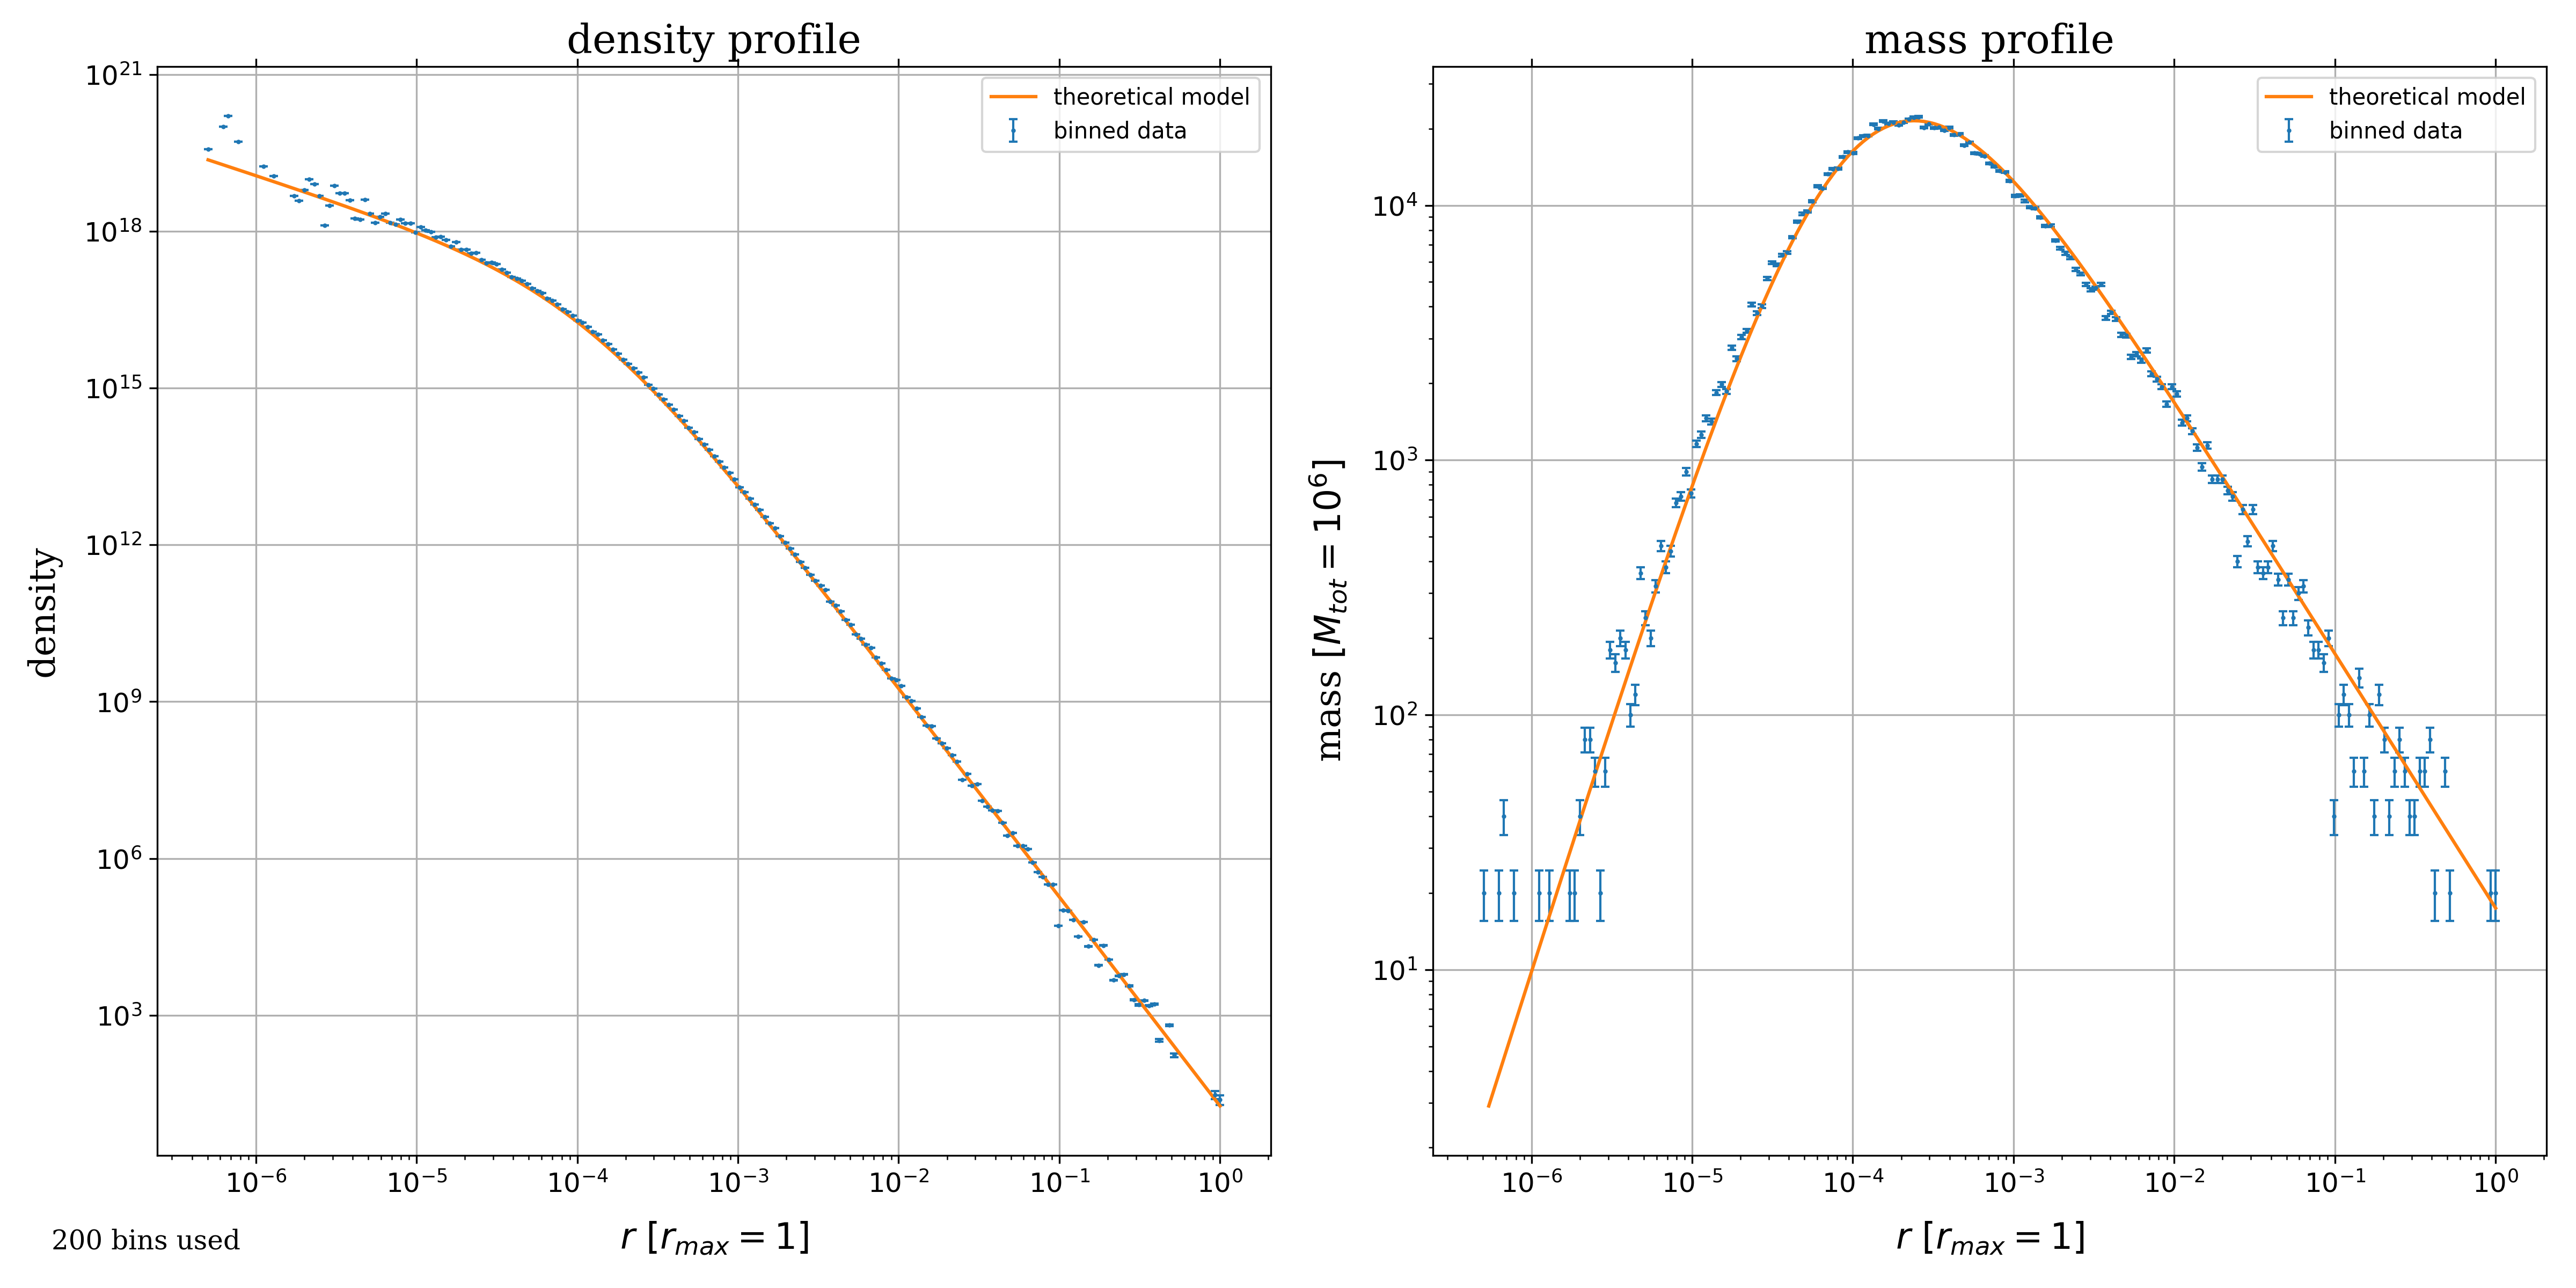
\includegraphics[width=\linewidth]{../results/density_plot/step0_density_plot.png}
	
	\alert{Only in this plot:} $M_{tot} \equiv 10^6$ so that the errorbars don't dominate the plot.
\end{frame}








\section{Piecewise Constant Method}

\begin{frame}
	\frametitle{Piecewise Constant Method: Donor-Cell Advection}
	
	\begin{columns}
		\column{0.6\textwidth}
			Assume cell state within cell is constant.
			
			For $u = 1$:
			\begin{align*}
			\rho_i ^{n+1} &= \rho_i^{n} + 
			\frac{\Delta t}{\Delta x} (f_{i-\half}^{n+\half} - f_{i+\half}^{n+\half} )\\
			f_{i\pm\half}^{n+1} &= u_{i\pm\half}\quad \rho_{i - \half \pm \half}
			\end{align*}
			
			First order accurate in time and space.
			
		\column{.4\textwidth}
			\centering
			\includegraphics[width=\textwidth]{images/donorcell.png}
			\tiny{
				Image adapted from ``Lecture Numerical Fluid Dynamics'', Lecture given by C.P. Dullemond and H.H. Wang at Heidelberg University, 2009
			}
		
	\end{columns}
\end{frame}	






\begin{frame}
	\vspace{10pt}
	\begin{columns}
		\column{.33\textwidth}
			\centering
			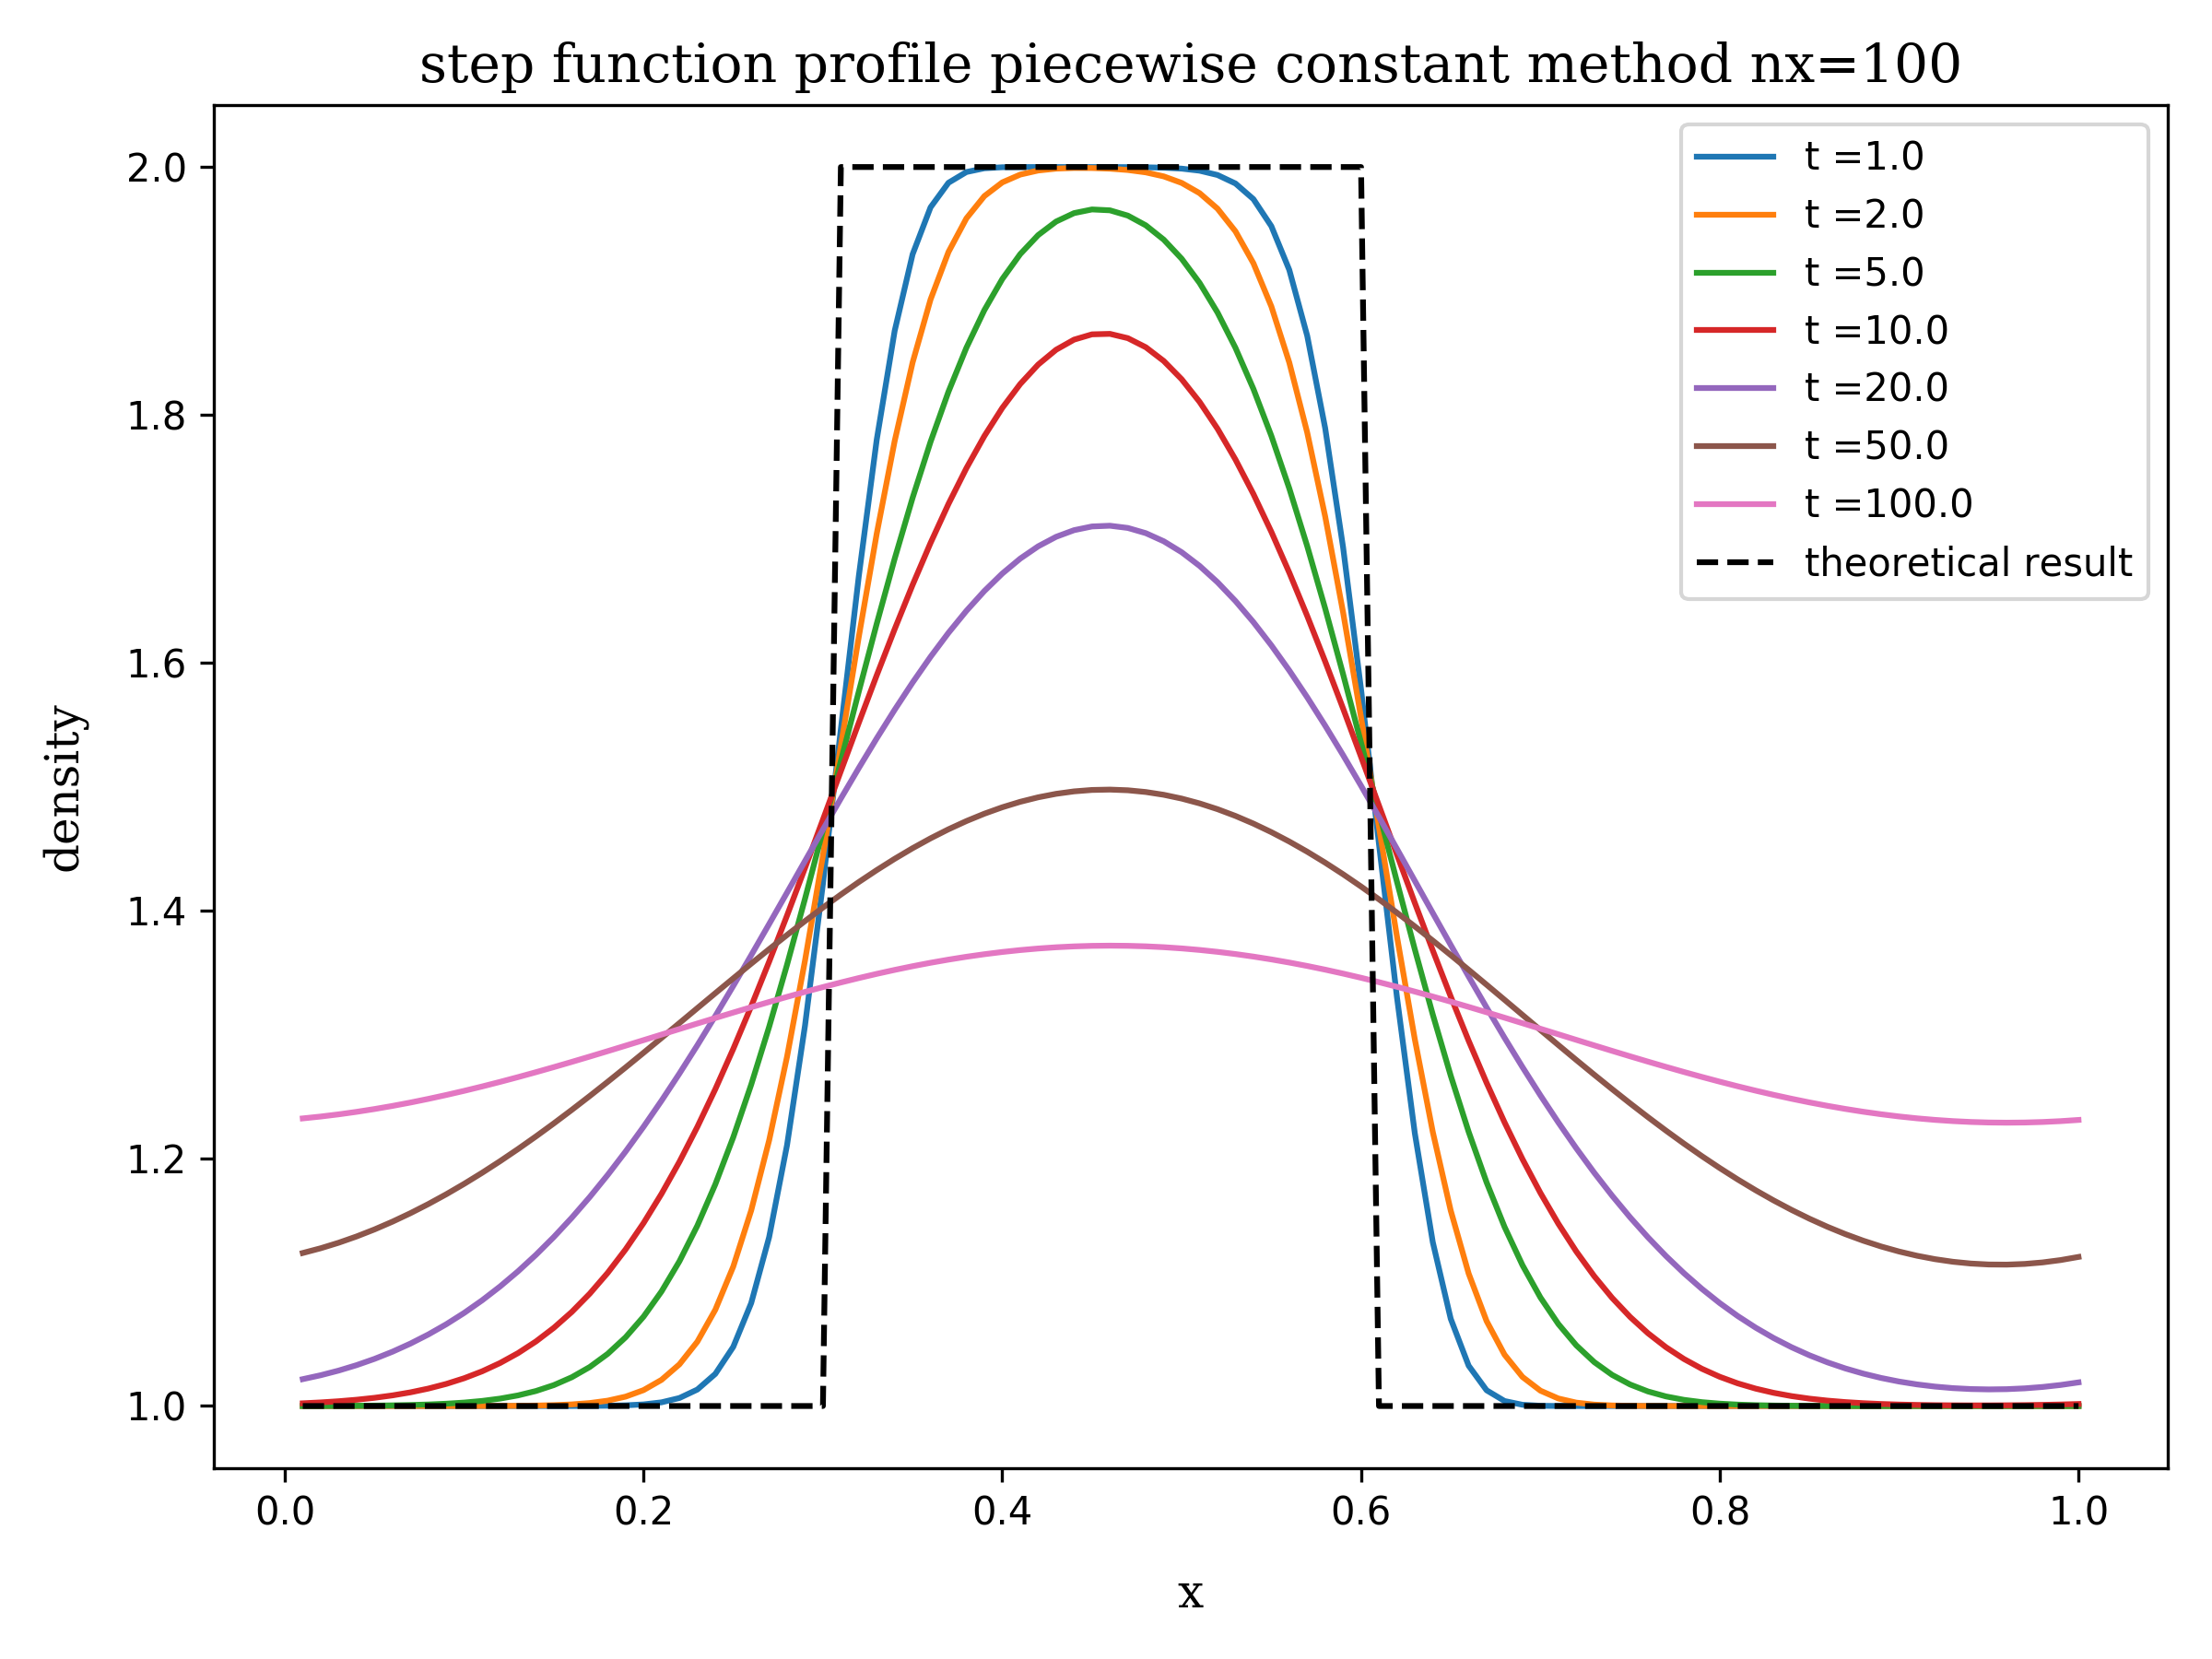
\includegraphics[height=.33\textheight]{../results/1D/pwconst/nx=100/plot_advection_step_function_pwconst_nx=100.png}\\
			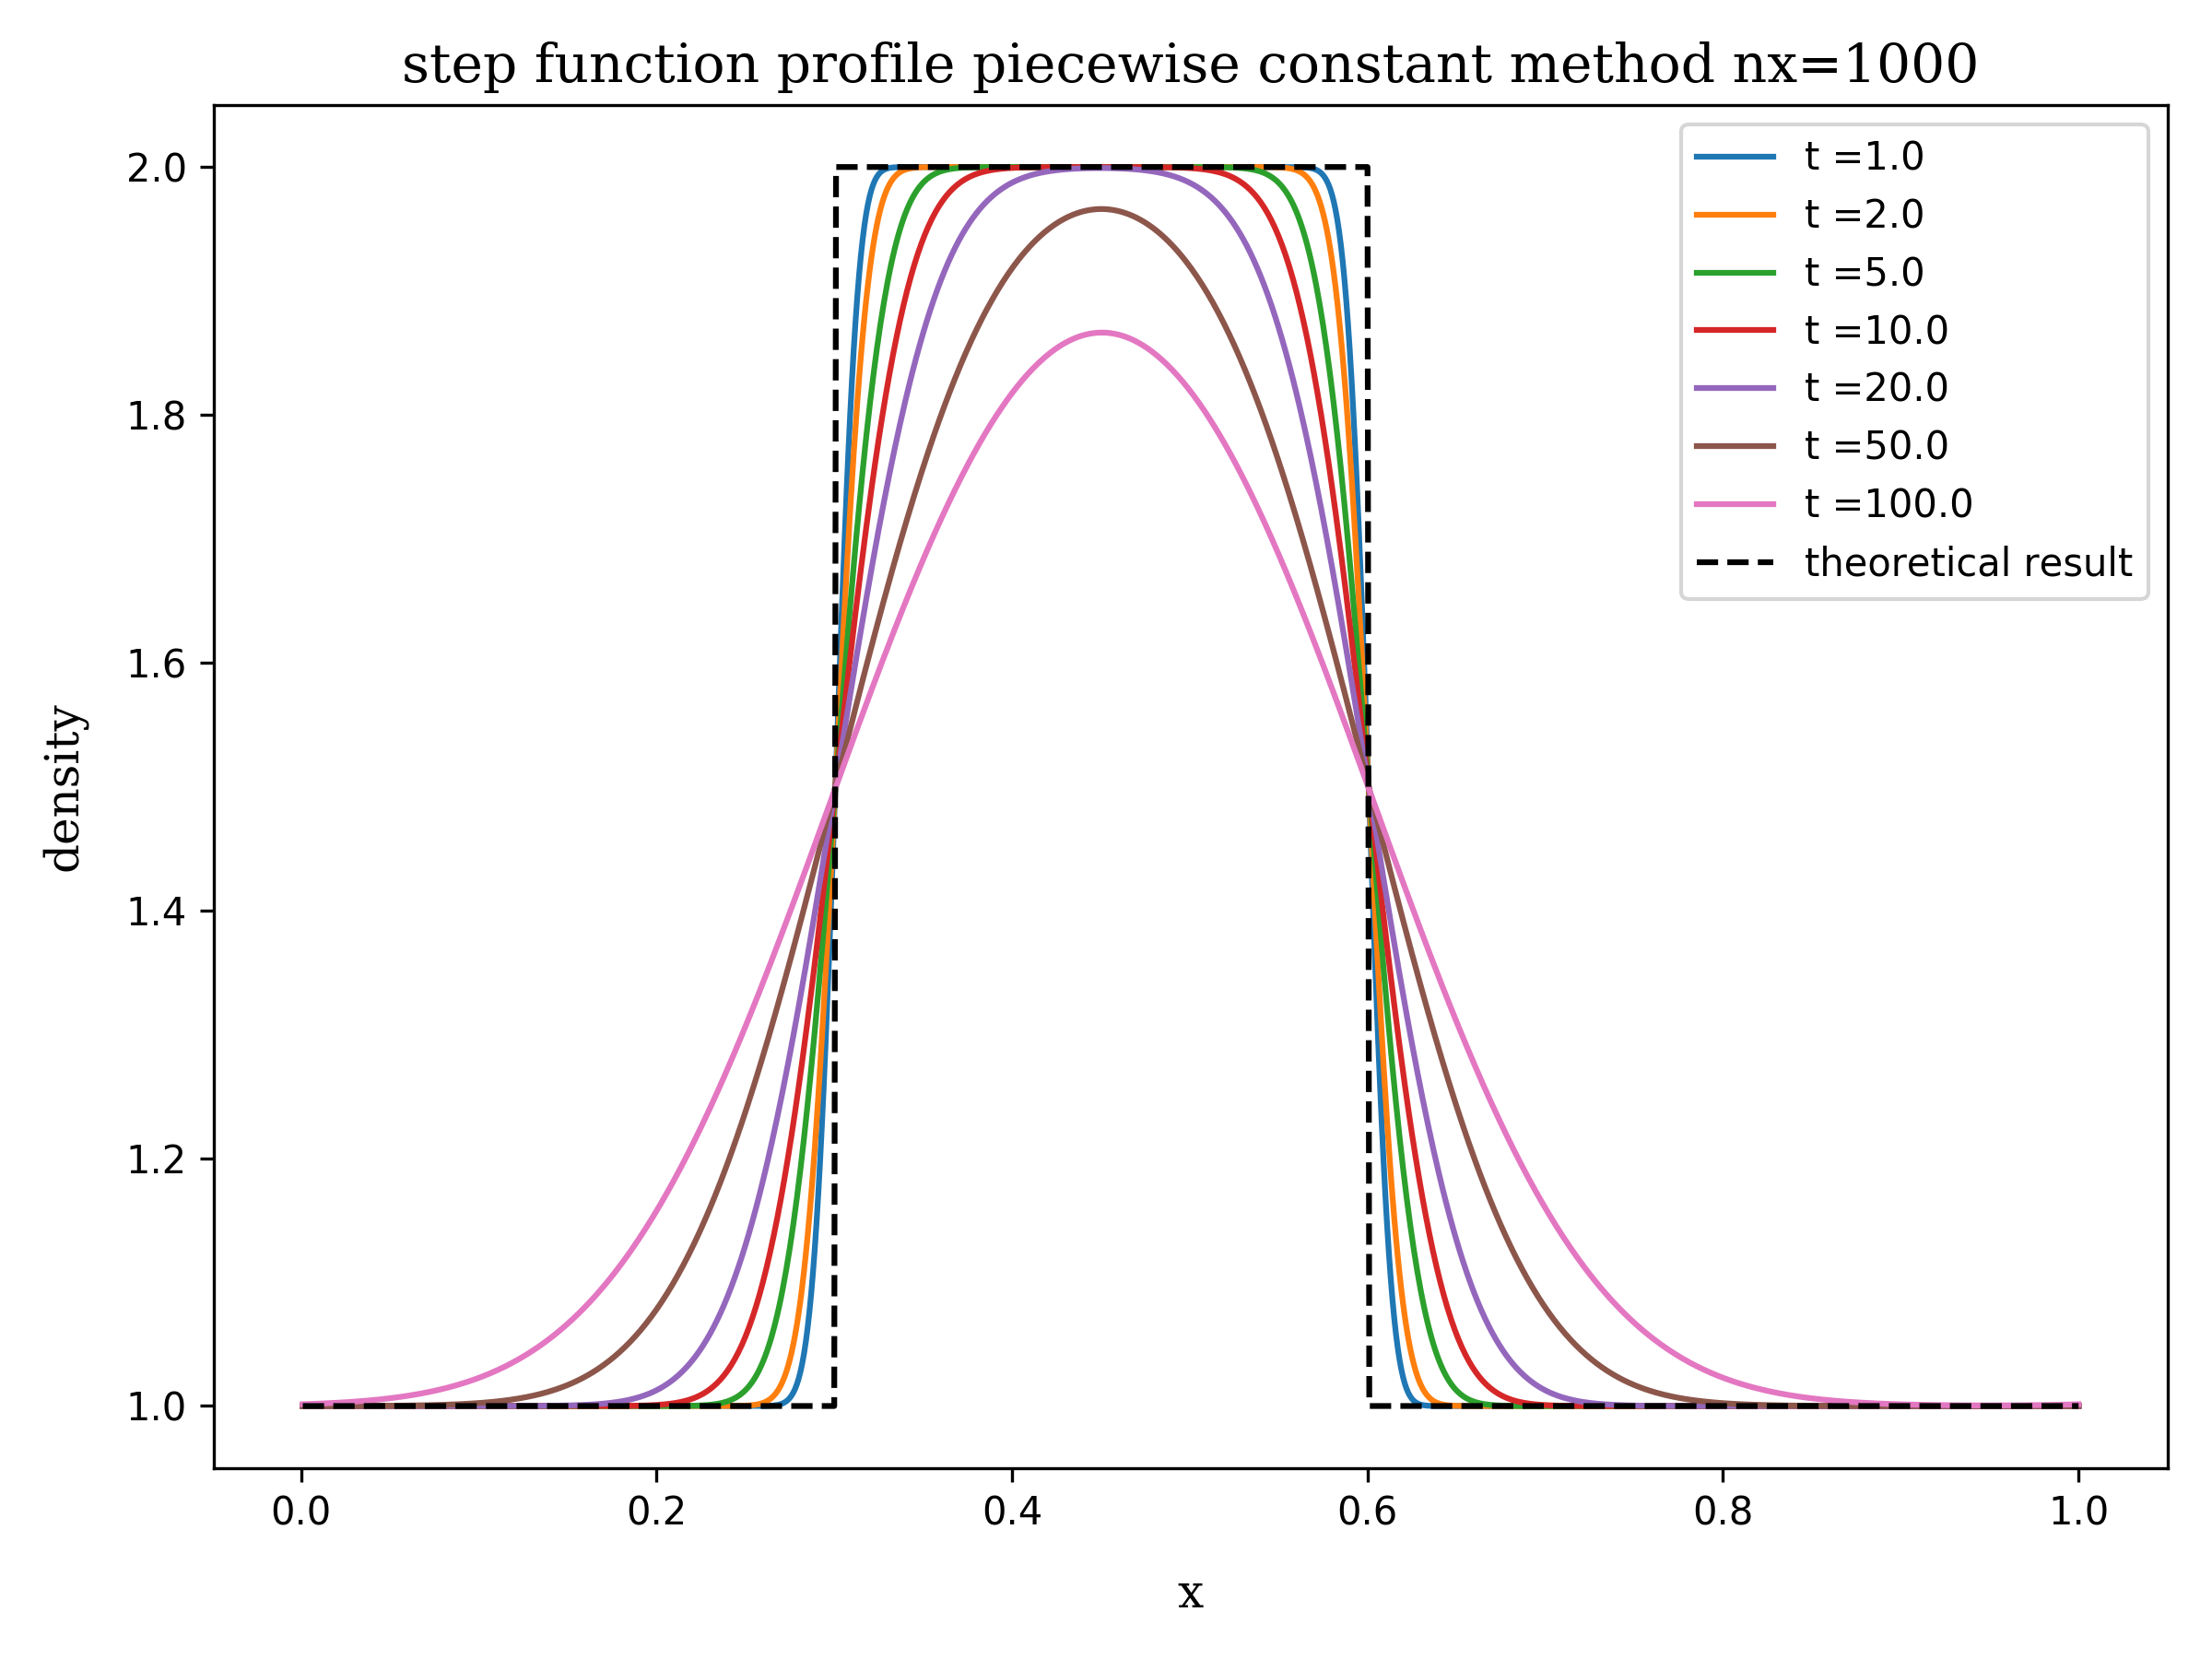
\includegraphics[height=.33\textheight]{../results/1D/pwconst/nx=1000/plot_advection_step_function_pwconst_nx=1000.png}\\
			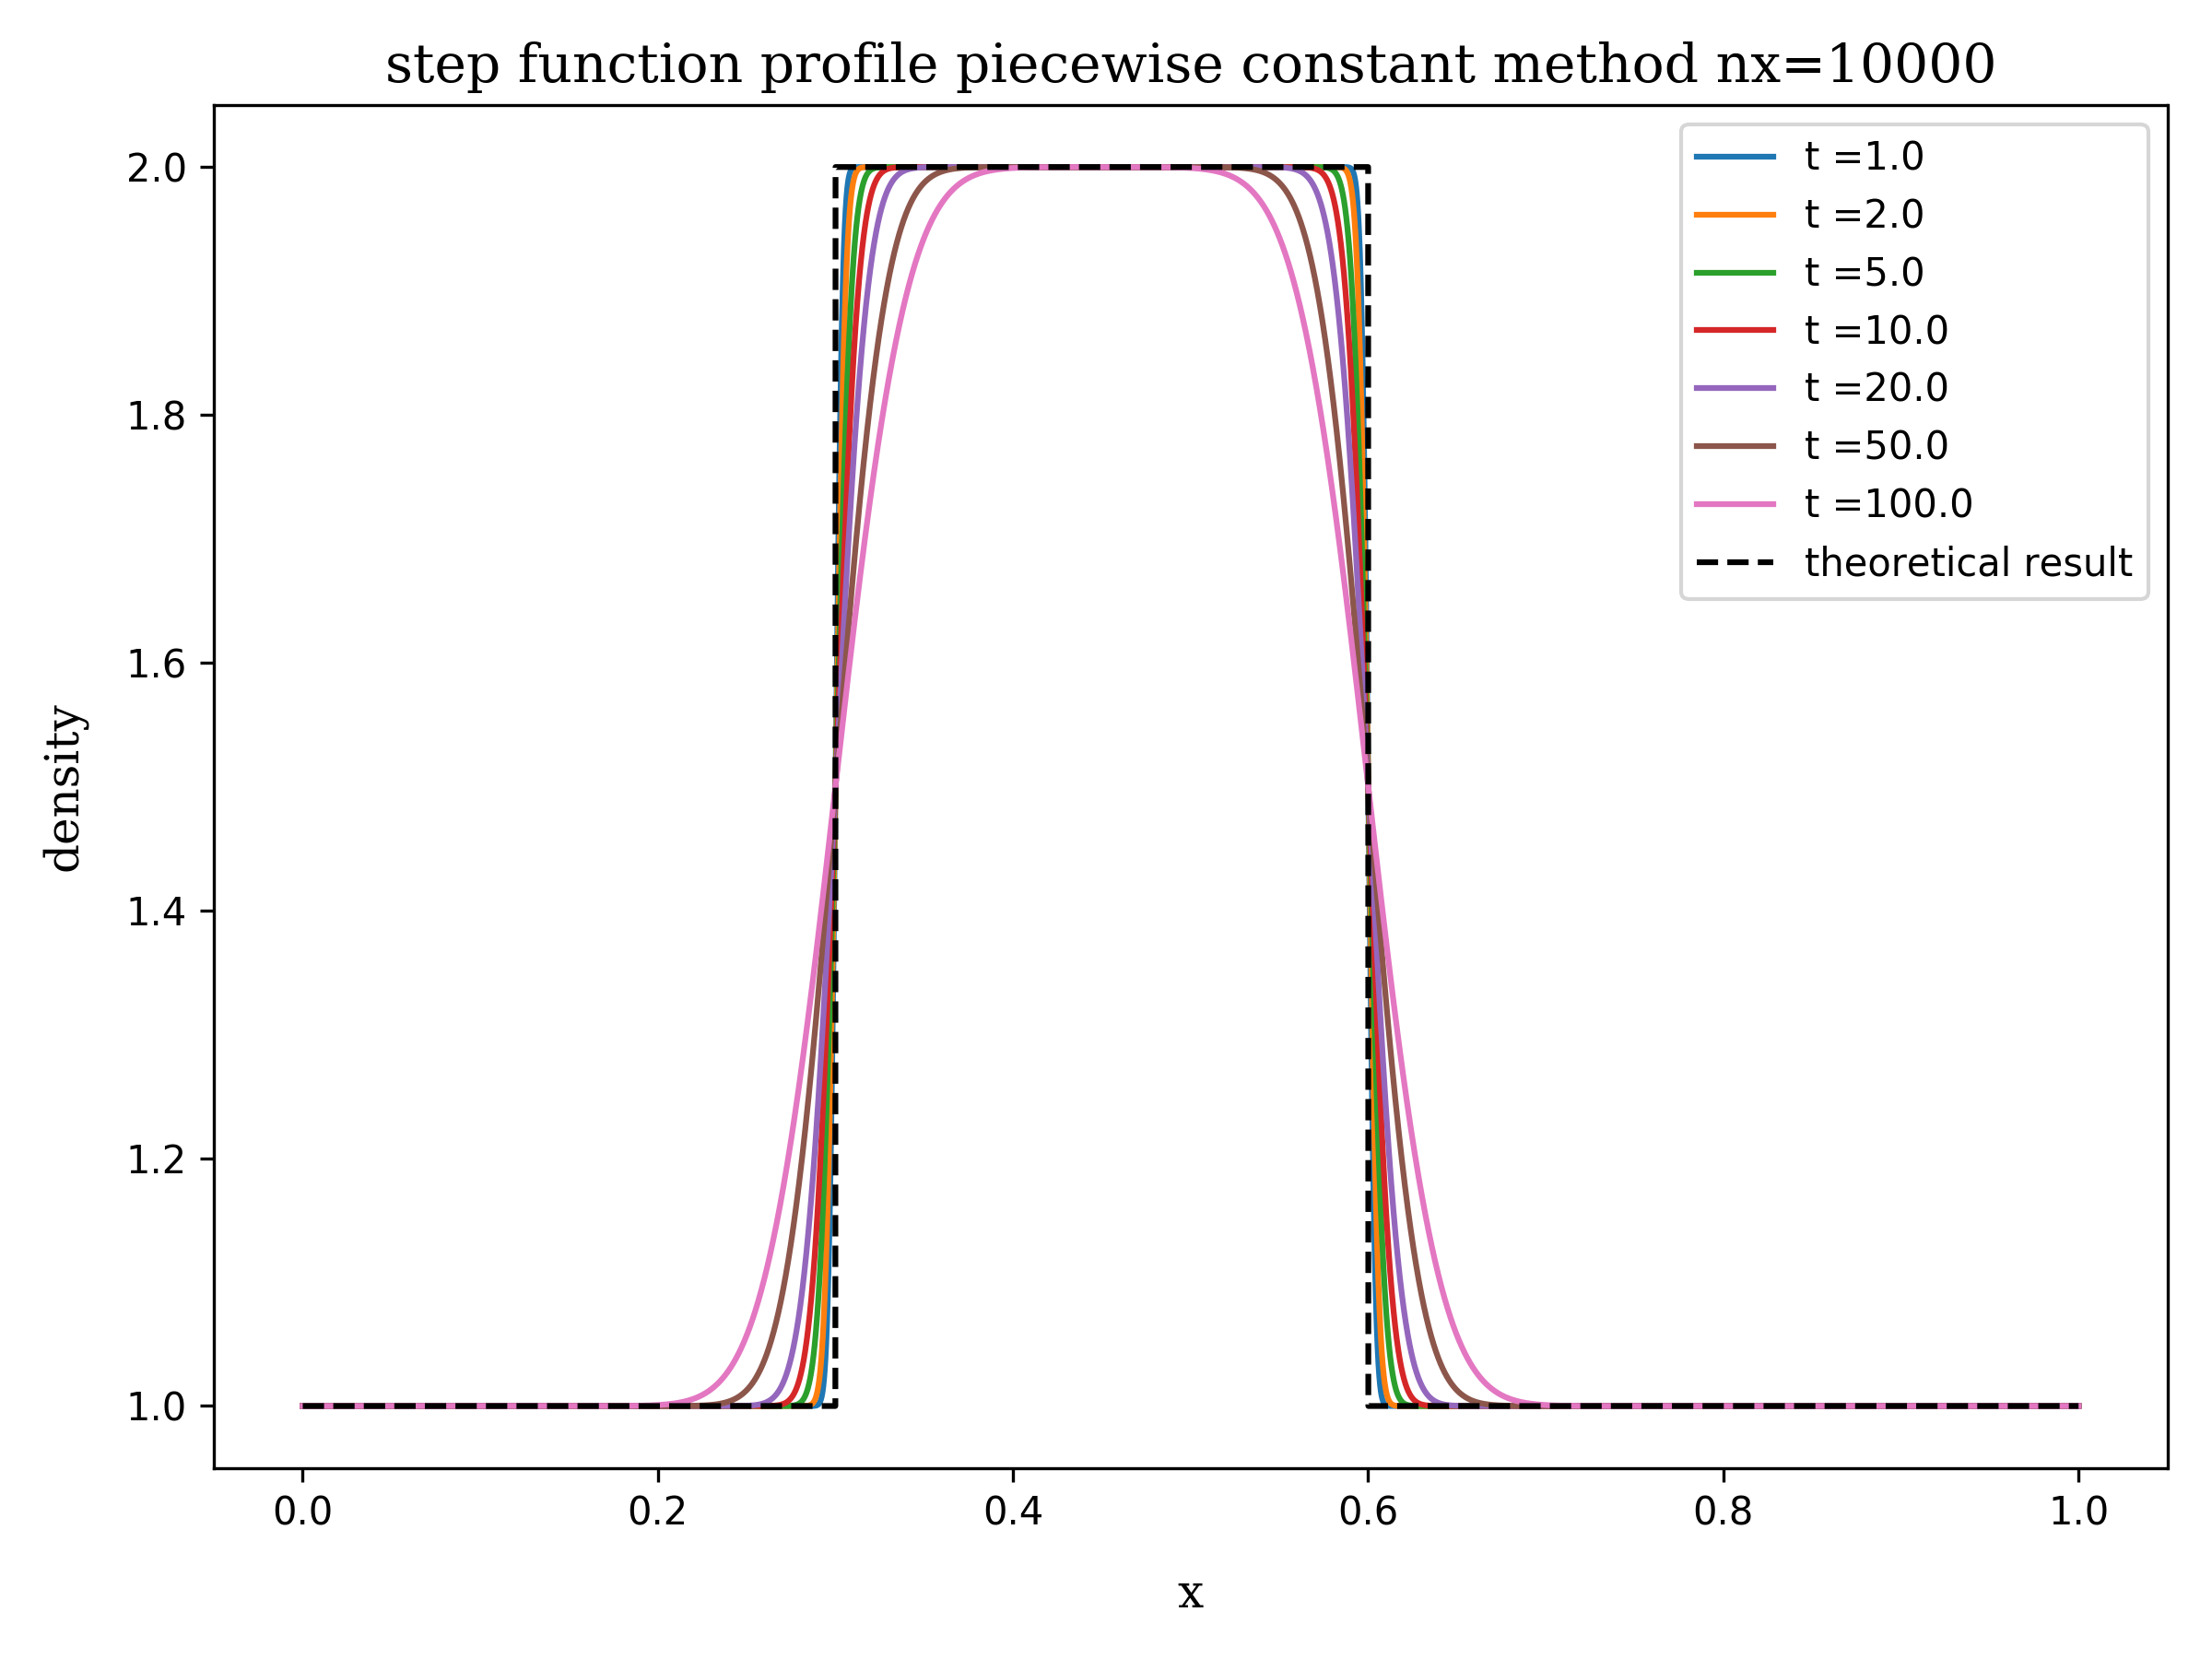
\includegraphics[height=.33\textheight]{../results/1D/pwconst/nx=10000/plot_advection_step_function_pwconst_nx=10000.png}
		\column{.33\textwidth}
			\centering
			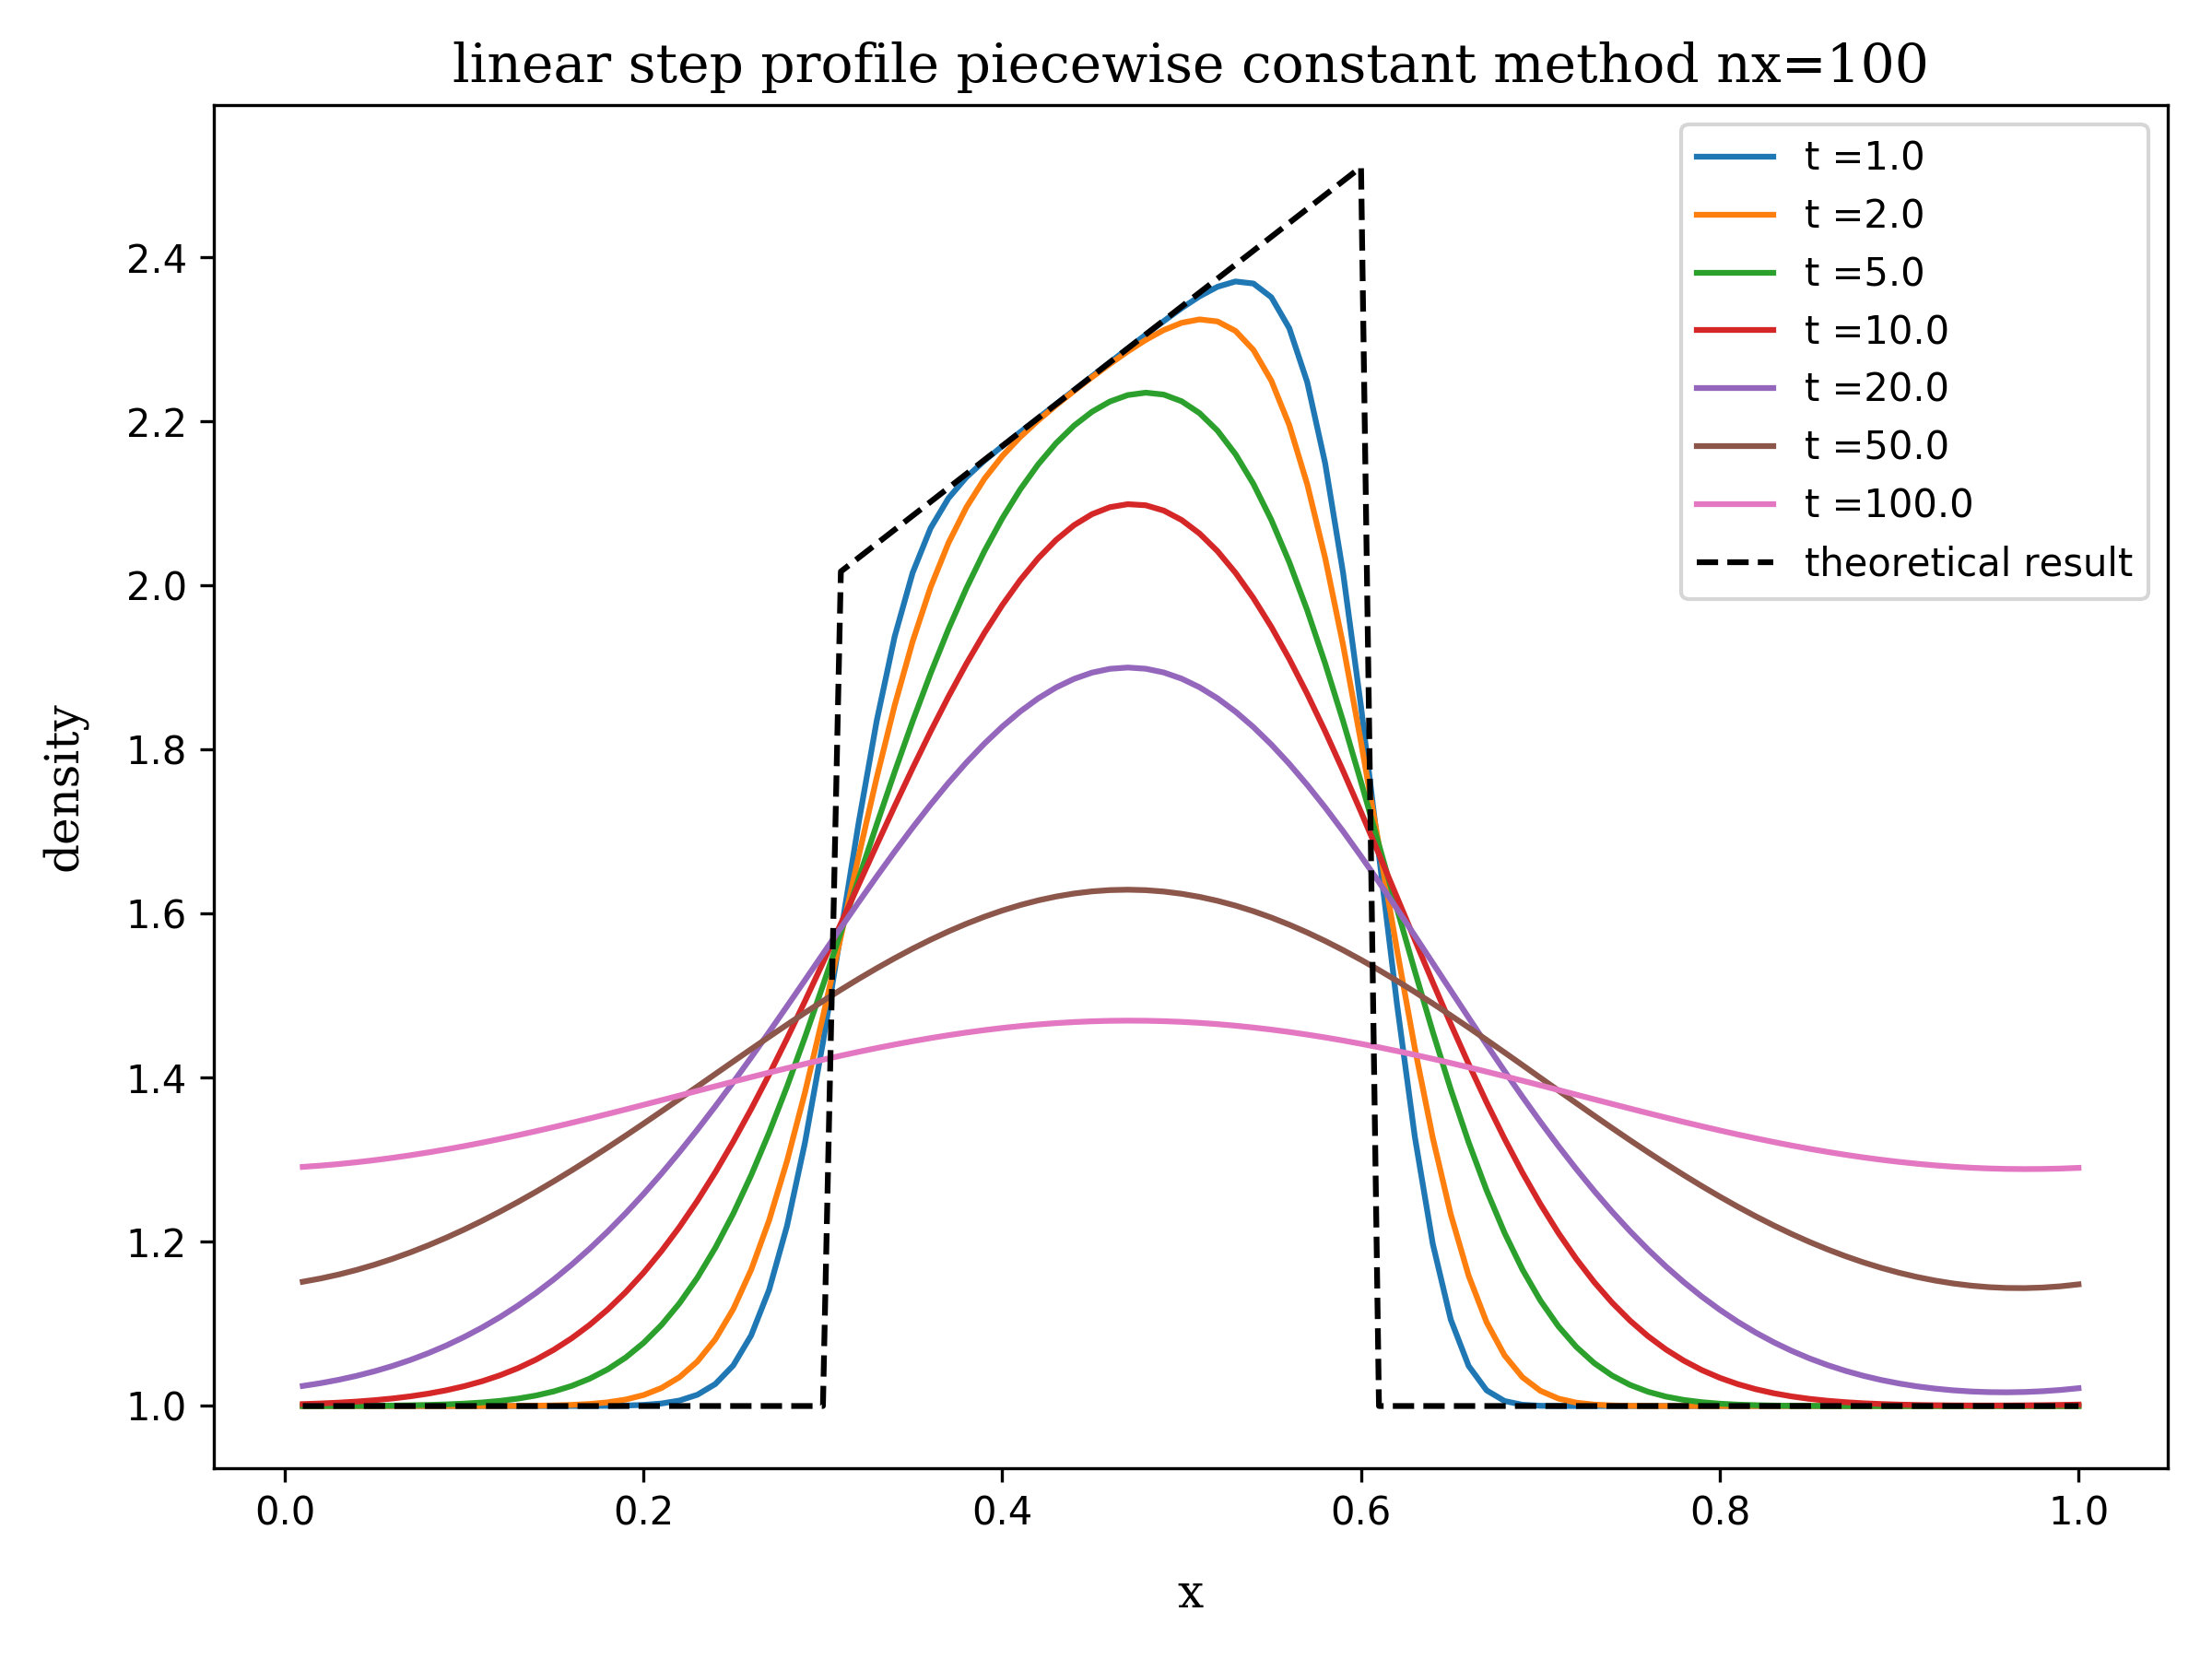
\includegraphics[height=.33\textheight]{../results/1D/pwconst/nx=100/plot_advection_linear_step_pwconst_nx=100.png}\\
			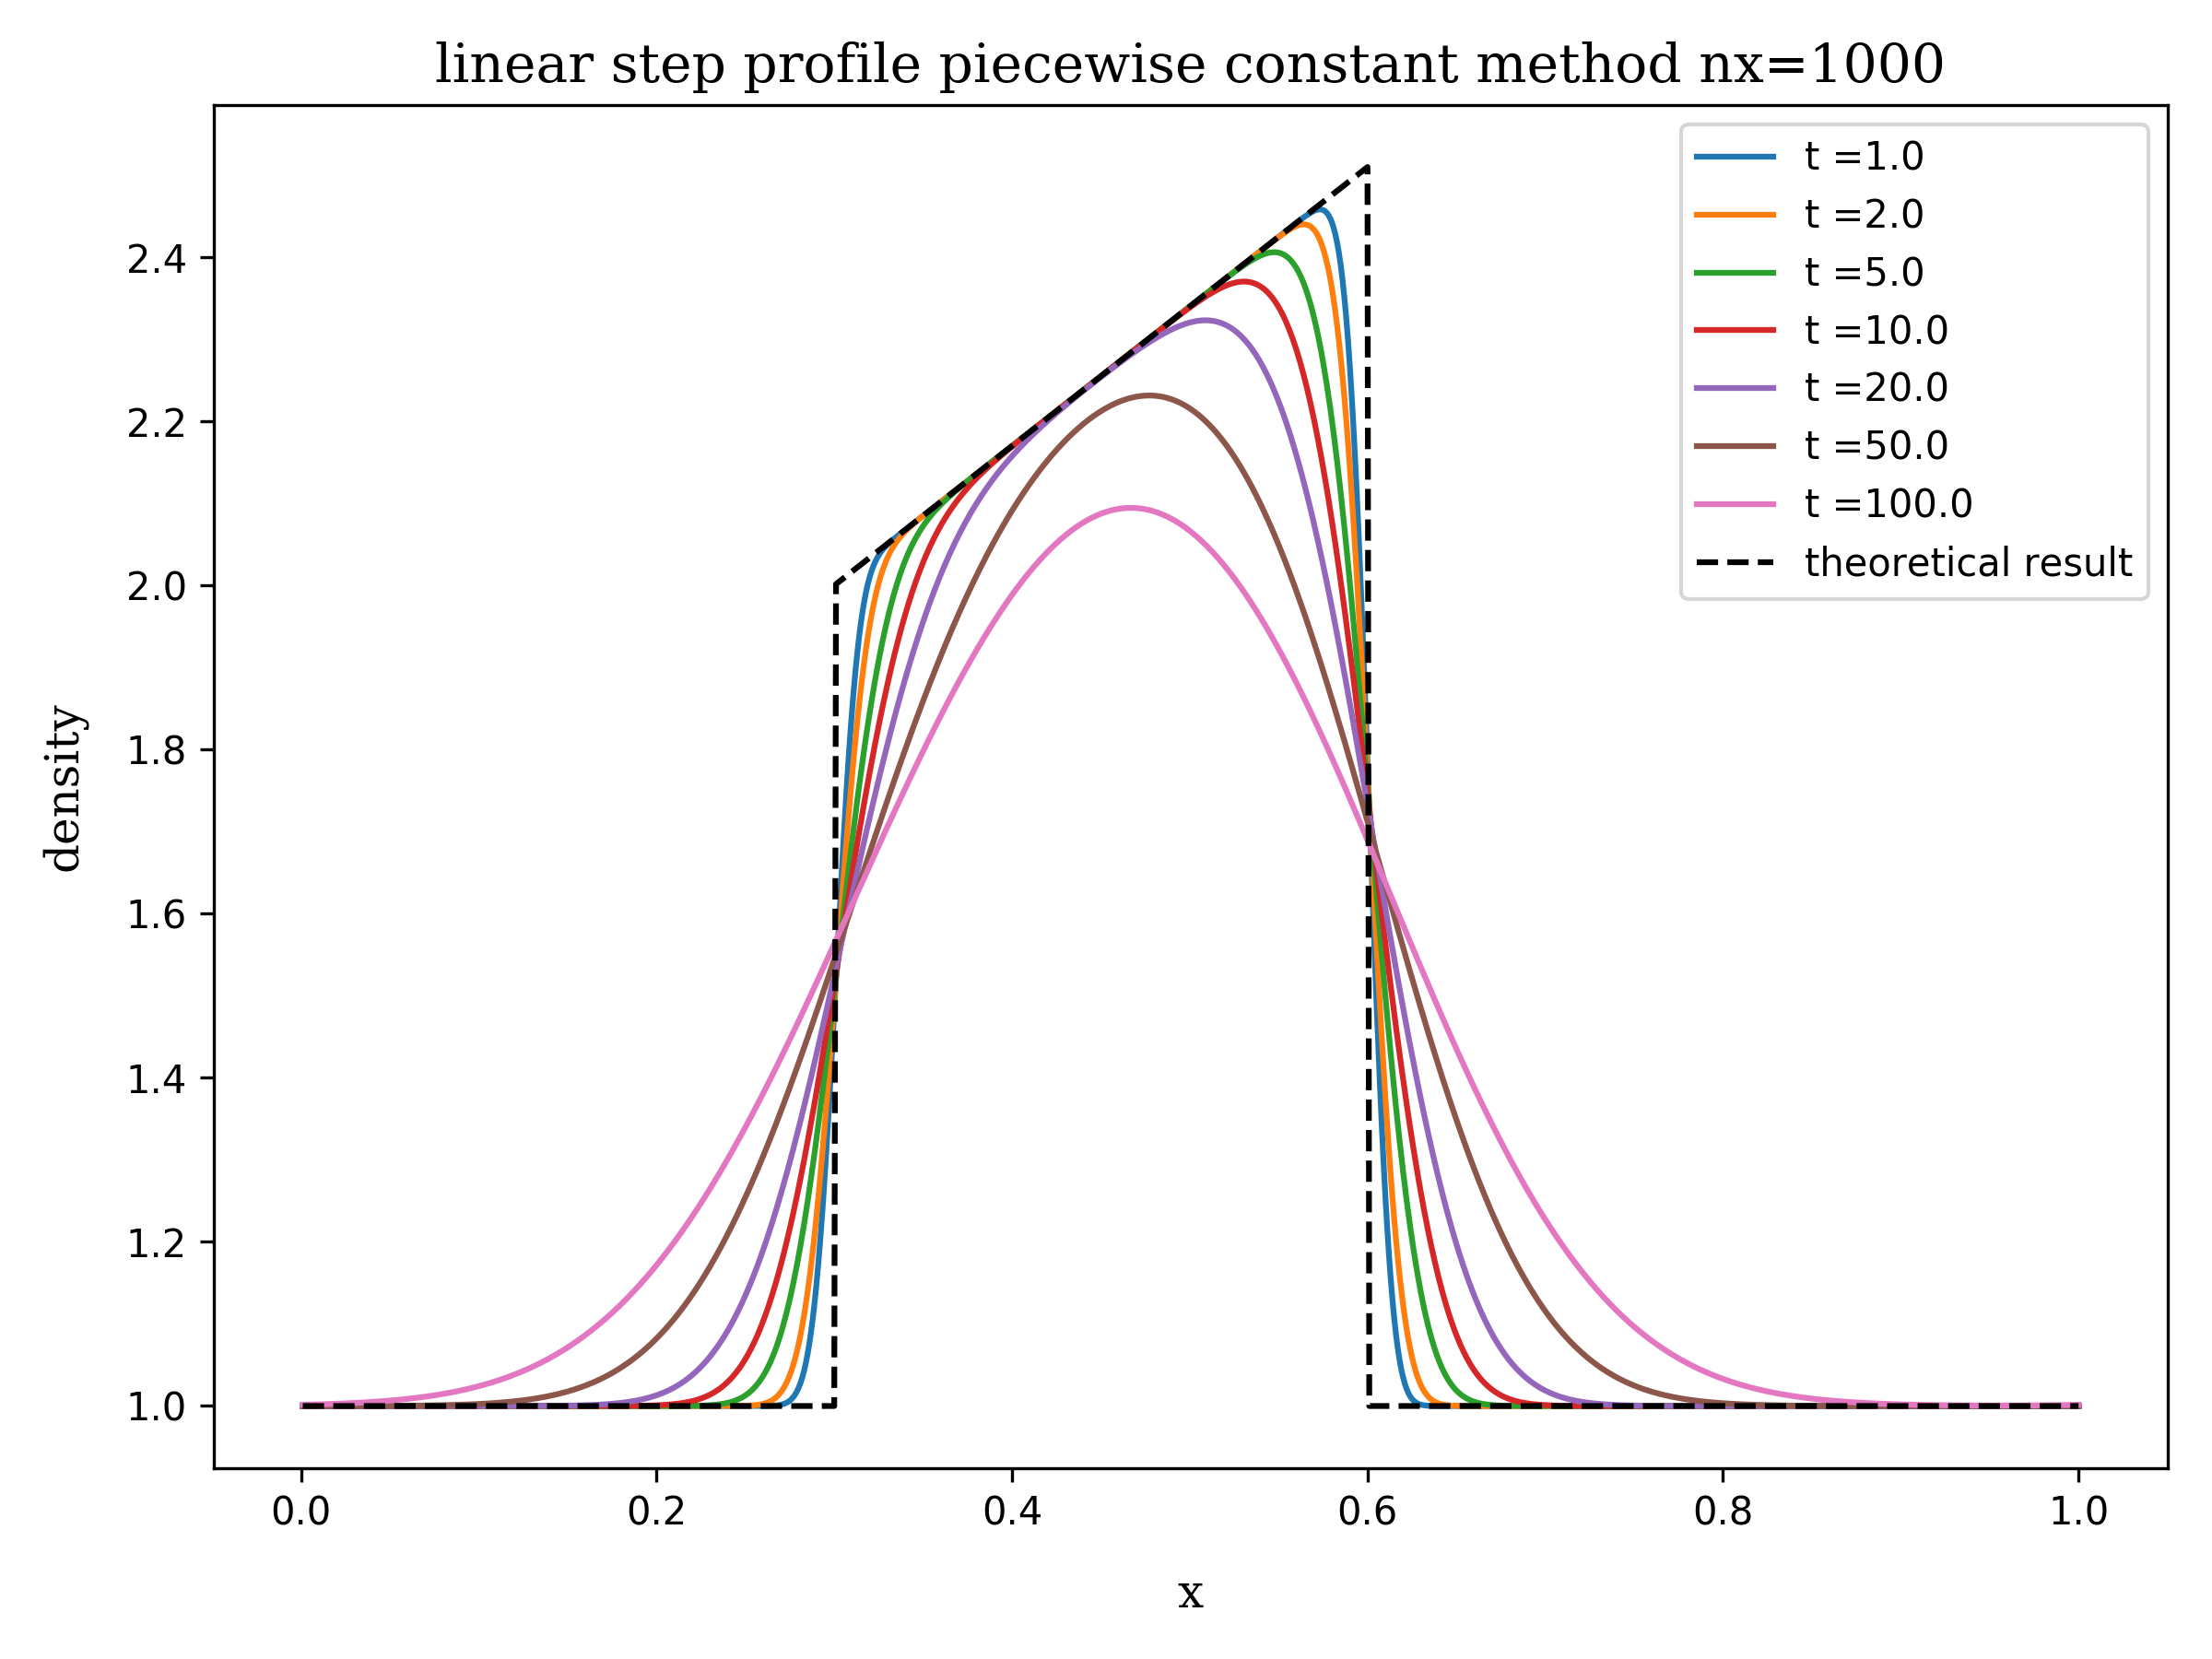
\includegraphics[height=.33\textheight]{../results/1D/pwconst/nx=1000/plot_advection_linear_step_pwconst_nx=1000.png}\\
			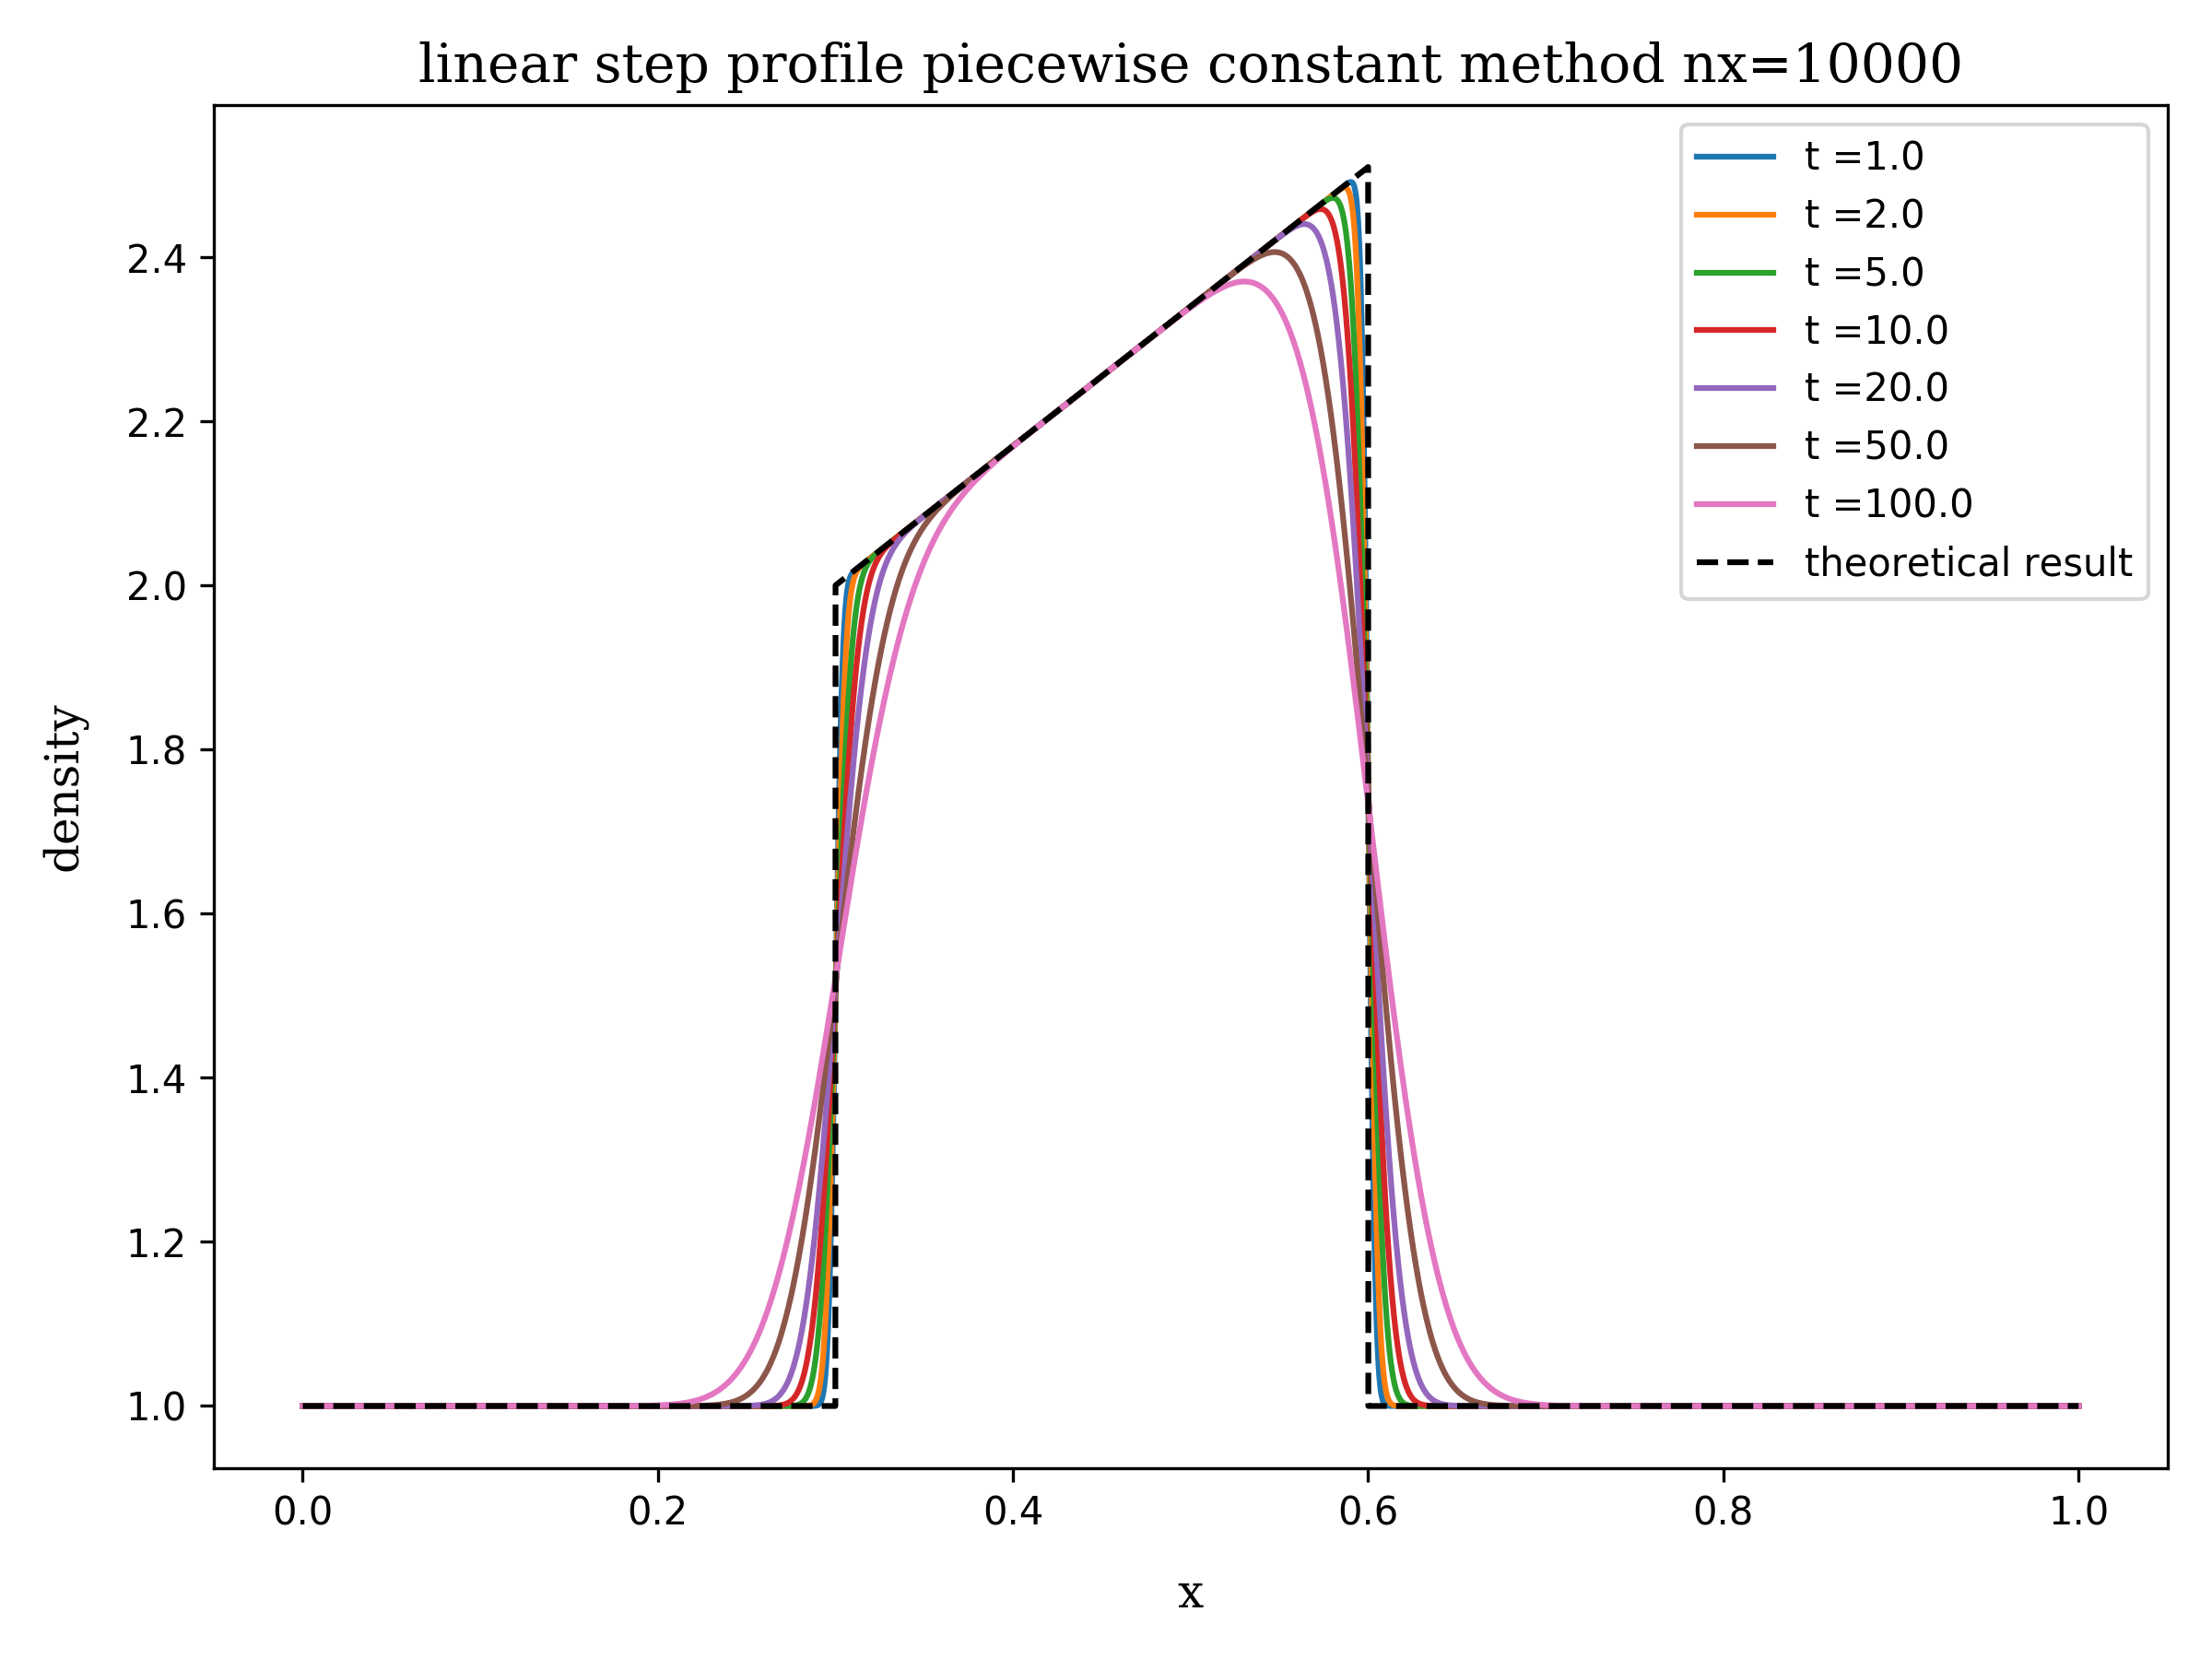
\includegraphics[height=.33\textheight]{../results/1D/pwconst/nx=10000/plot_advection_linear_step_pwconst_nx=10000.png}
		\column{.33\textwidth}
			\centering
			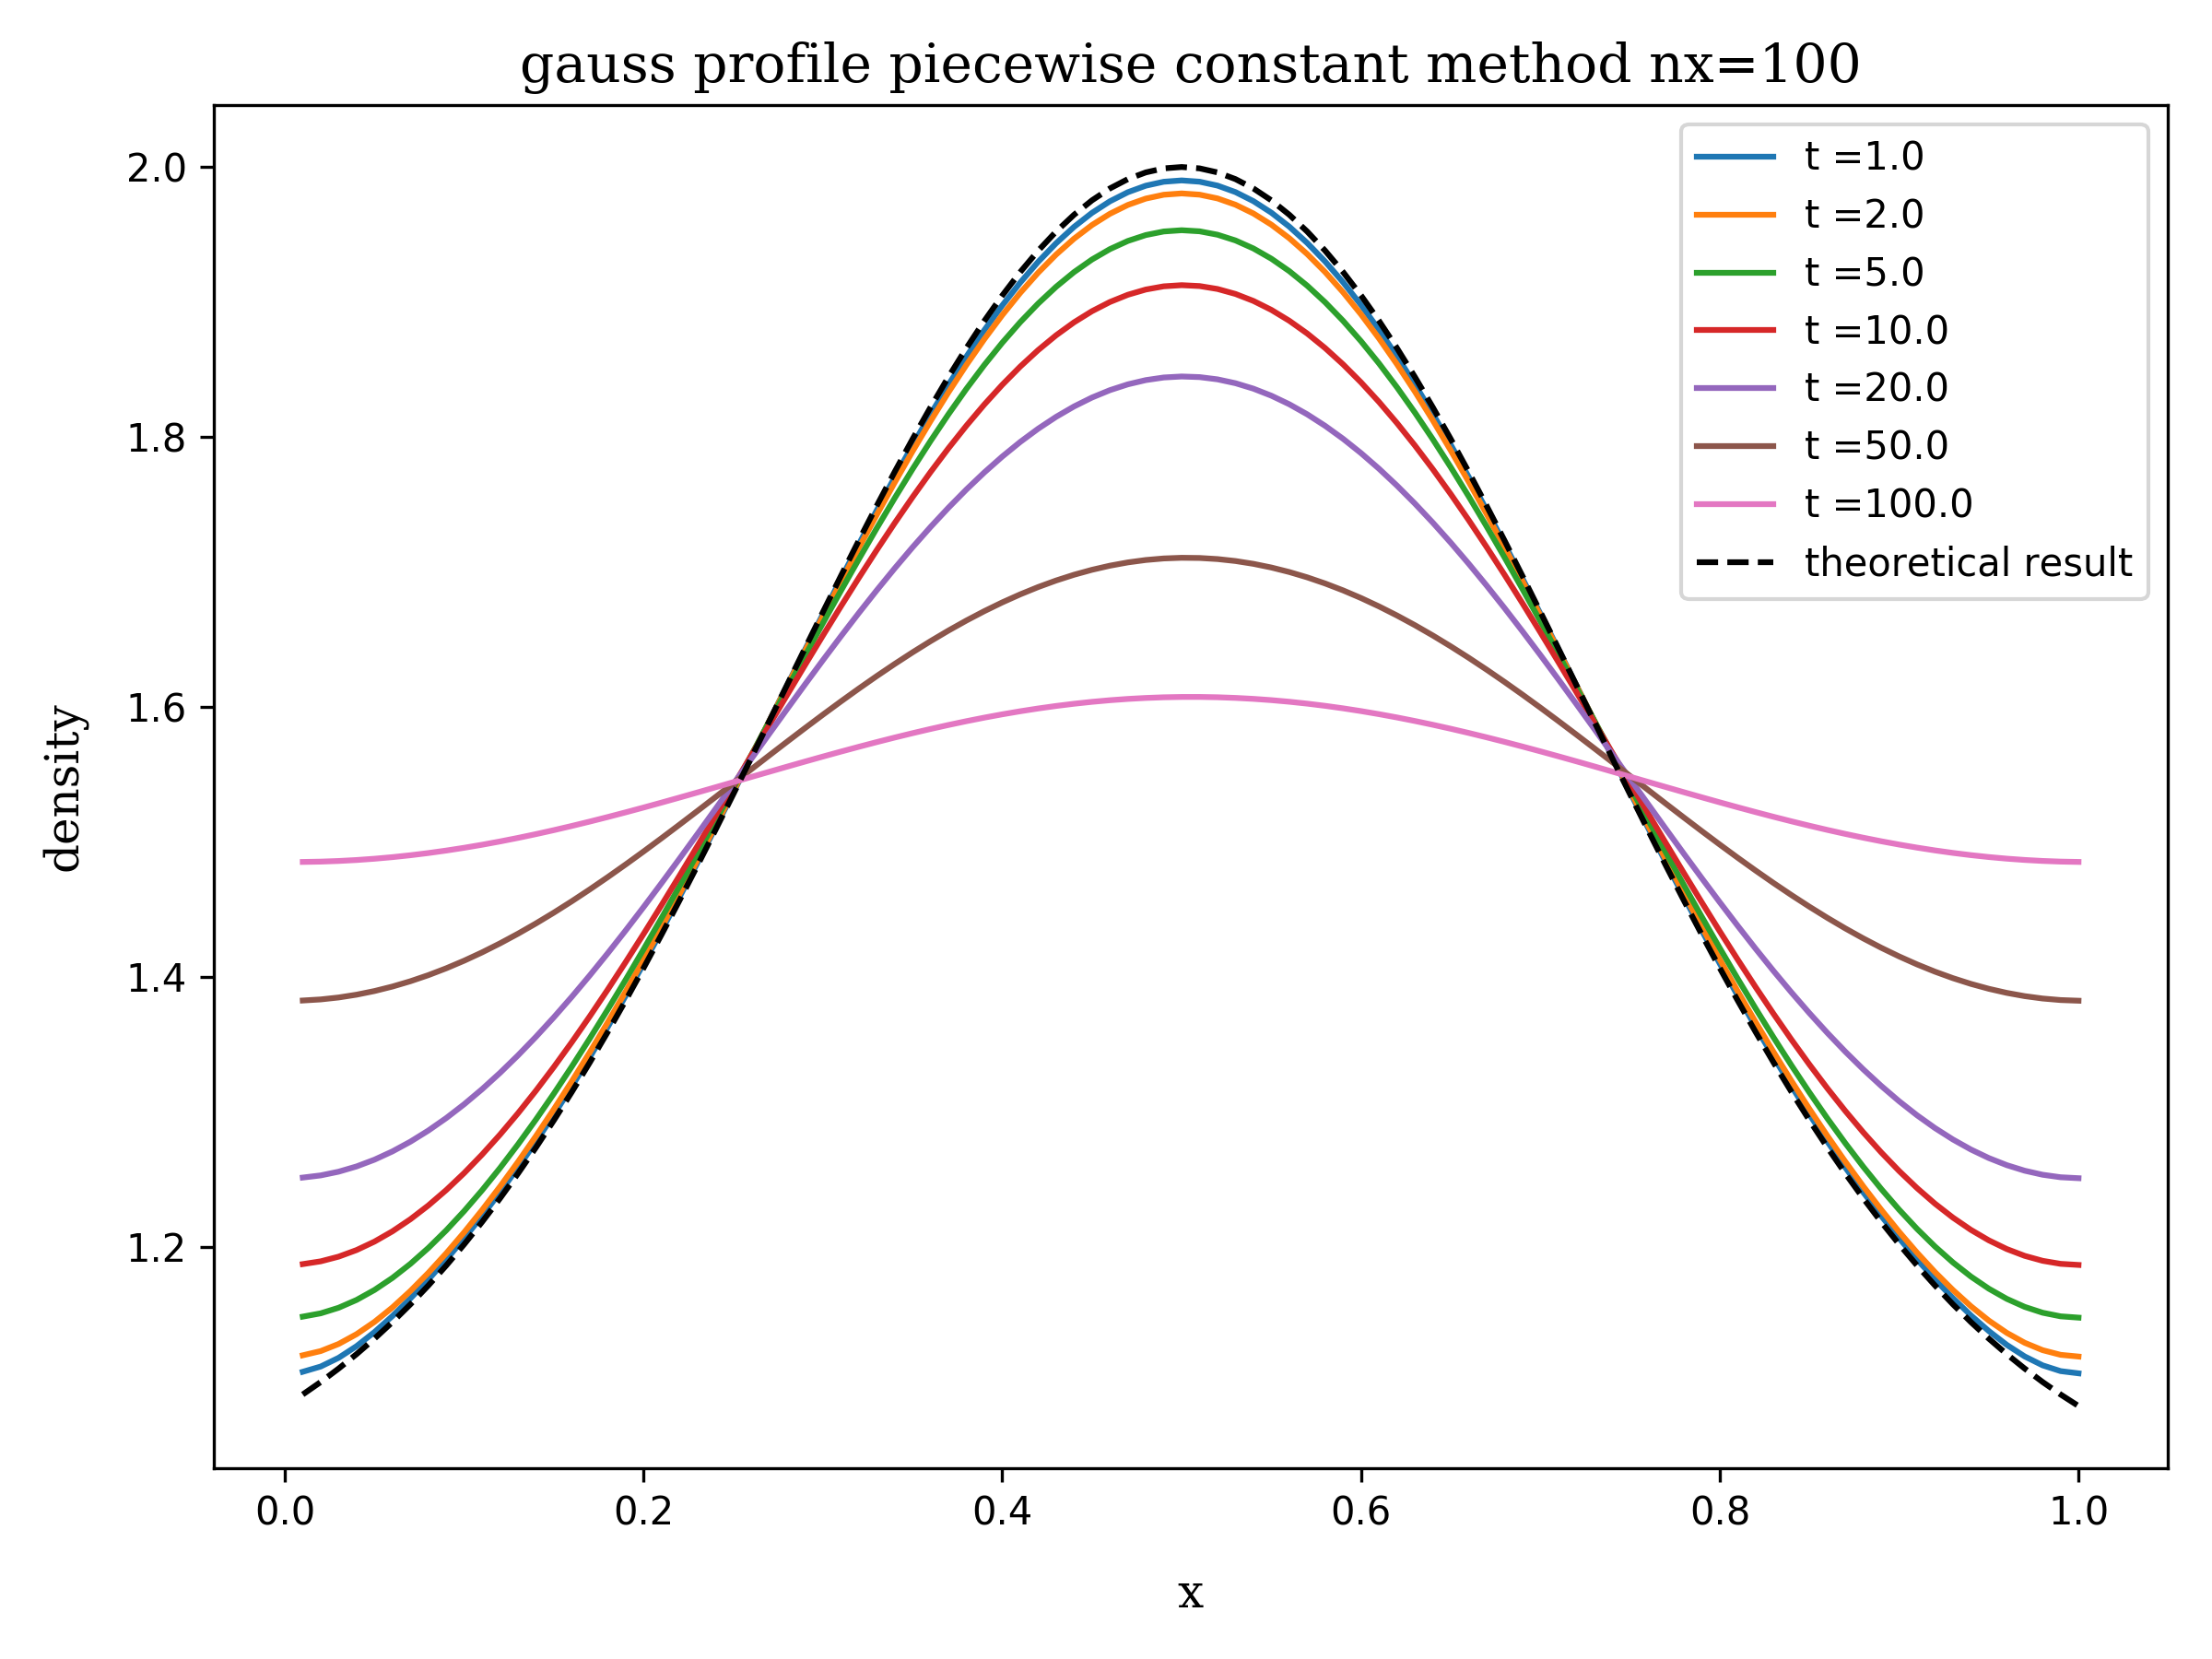
\includegraphics[height=.33\textheight]{../results/1D/pwconst/nx=100/plot_advection_gauss_pwconst_nx=100.png}\\
			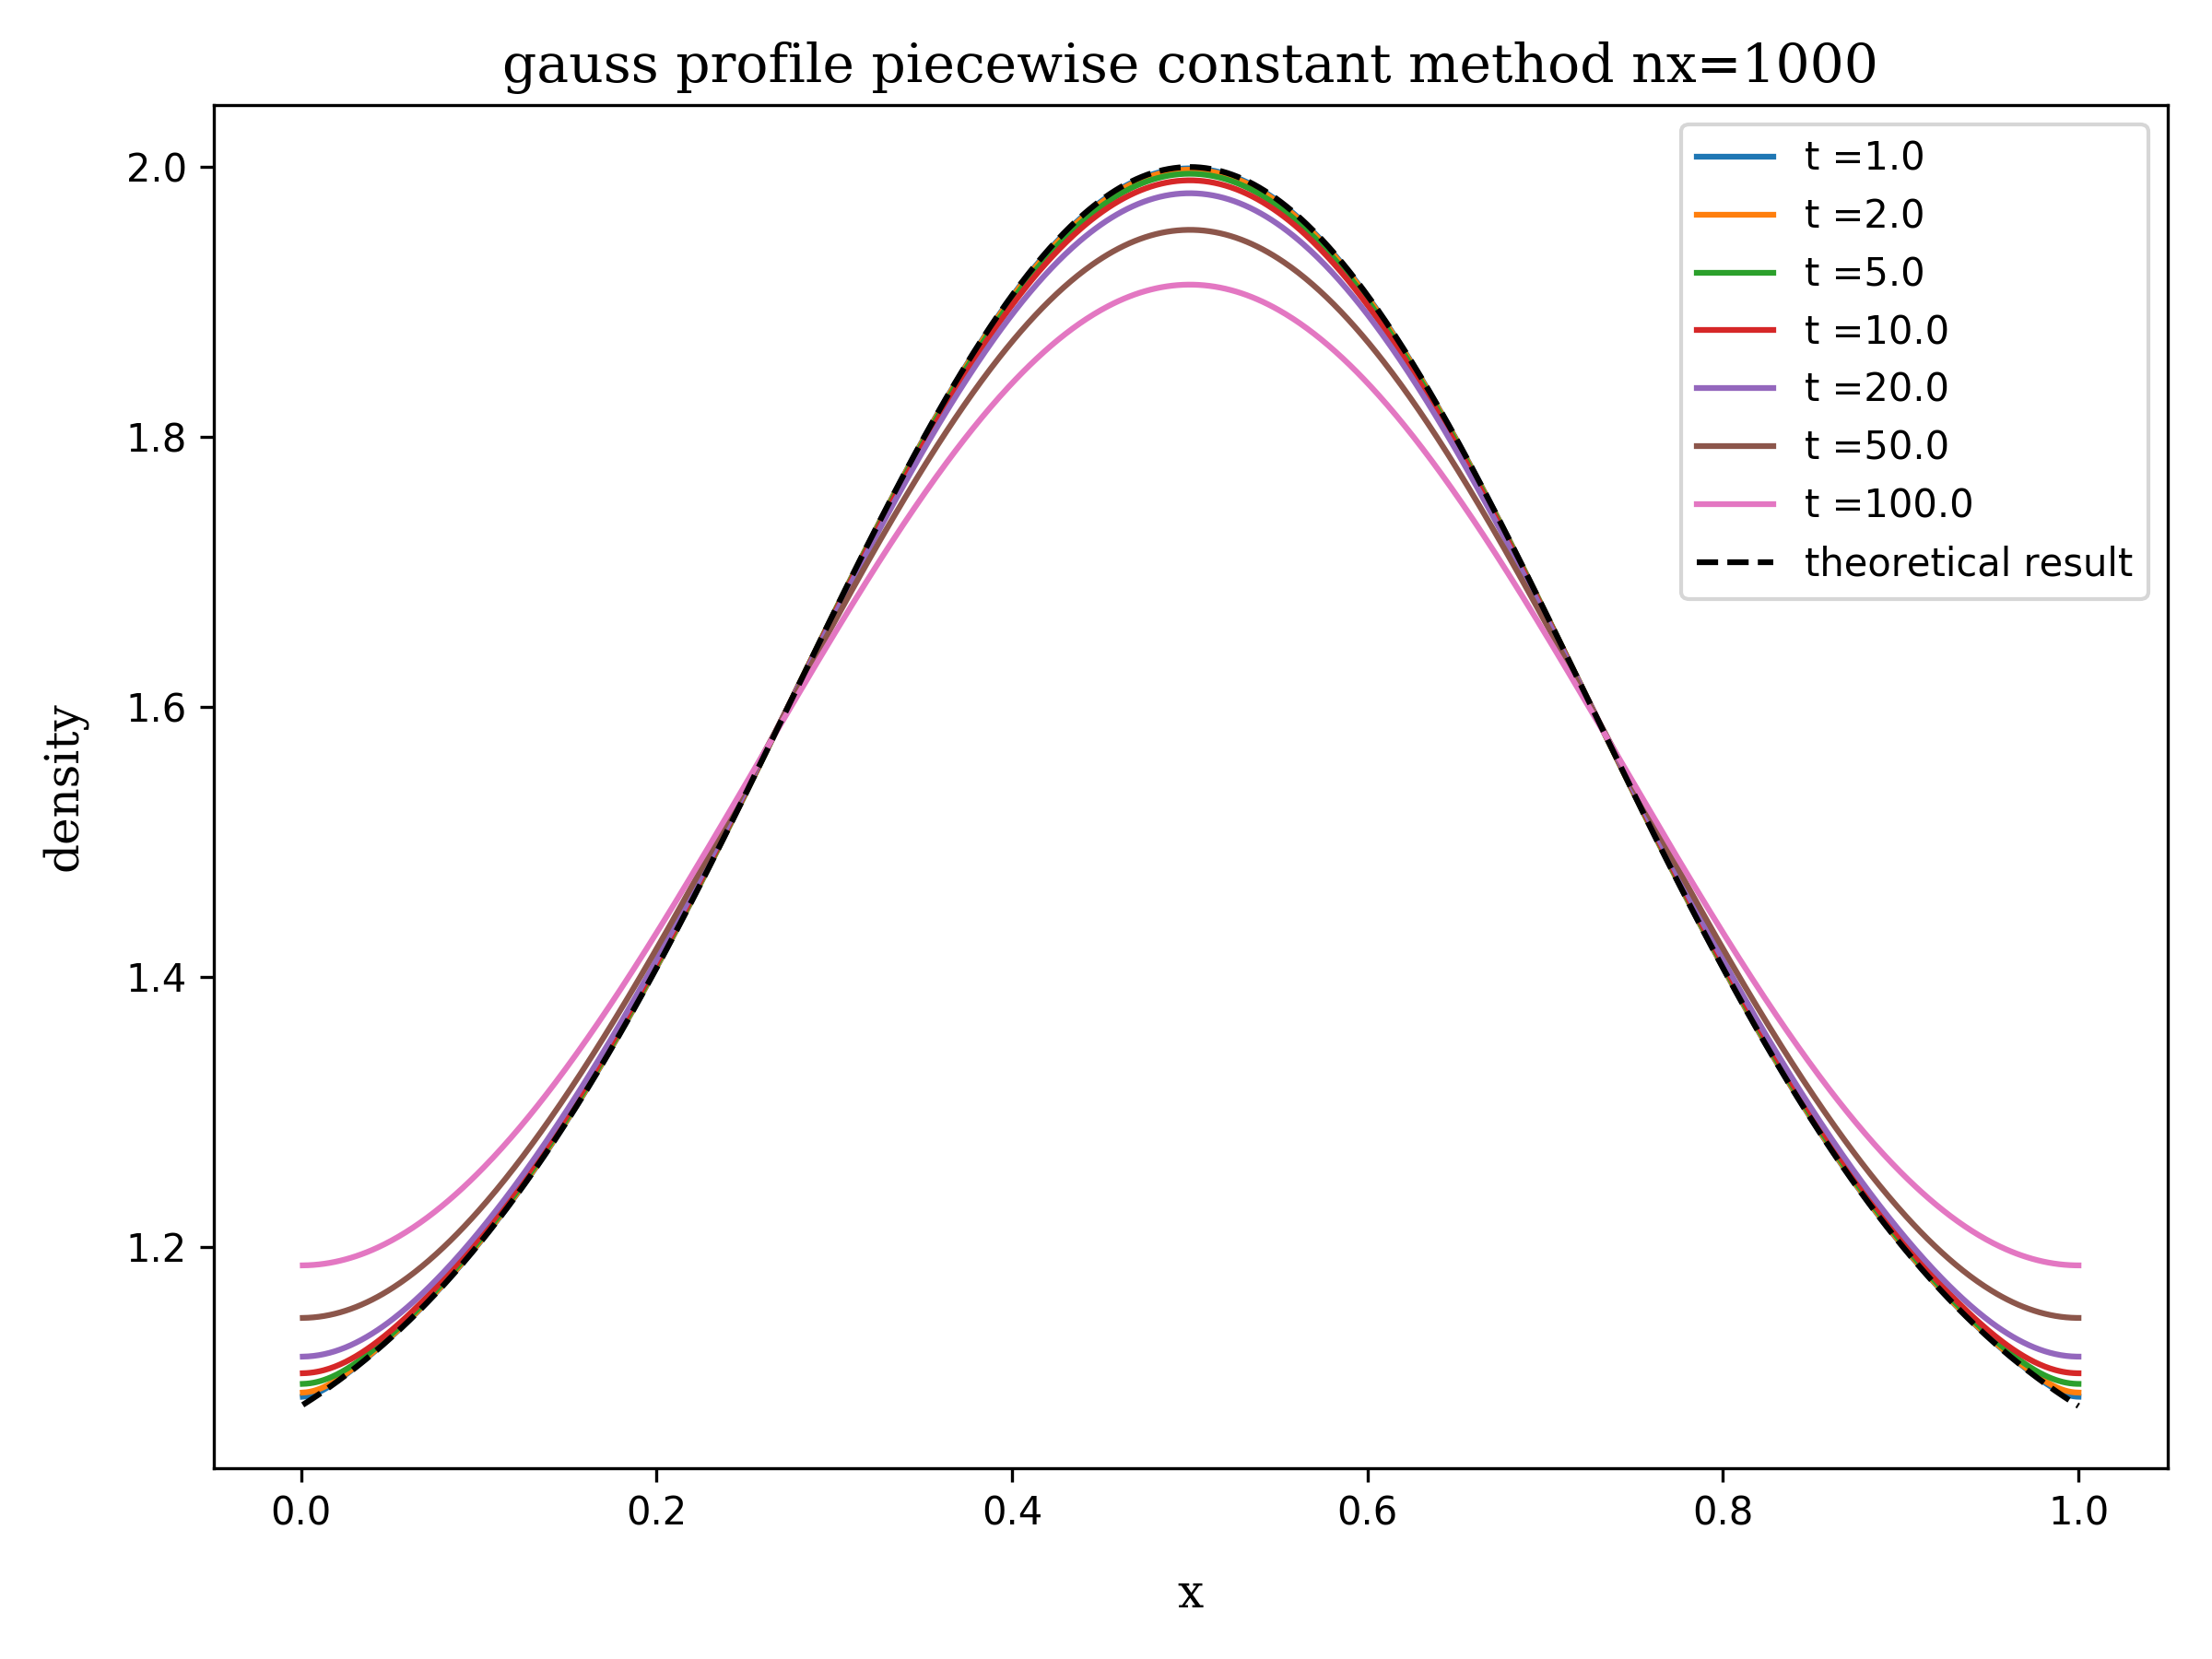
\includegraphics[height=.33\textheight]{../results/1D/pwconst/nx=1000/plot_advection_gauss_pwconst_nx=1000.png}\\
			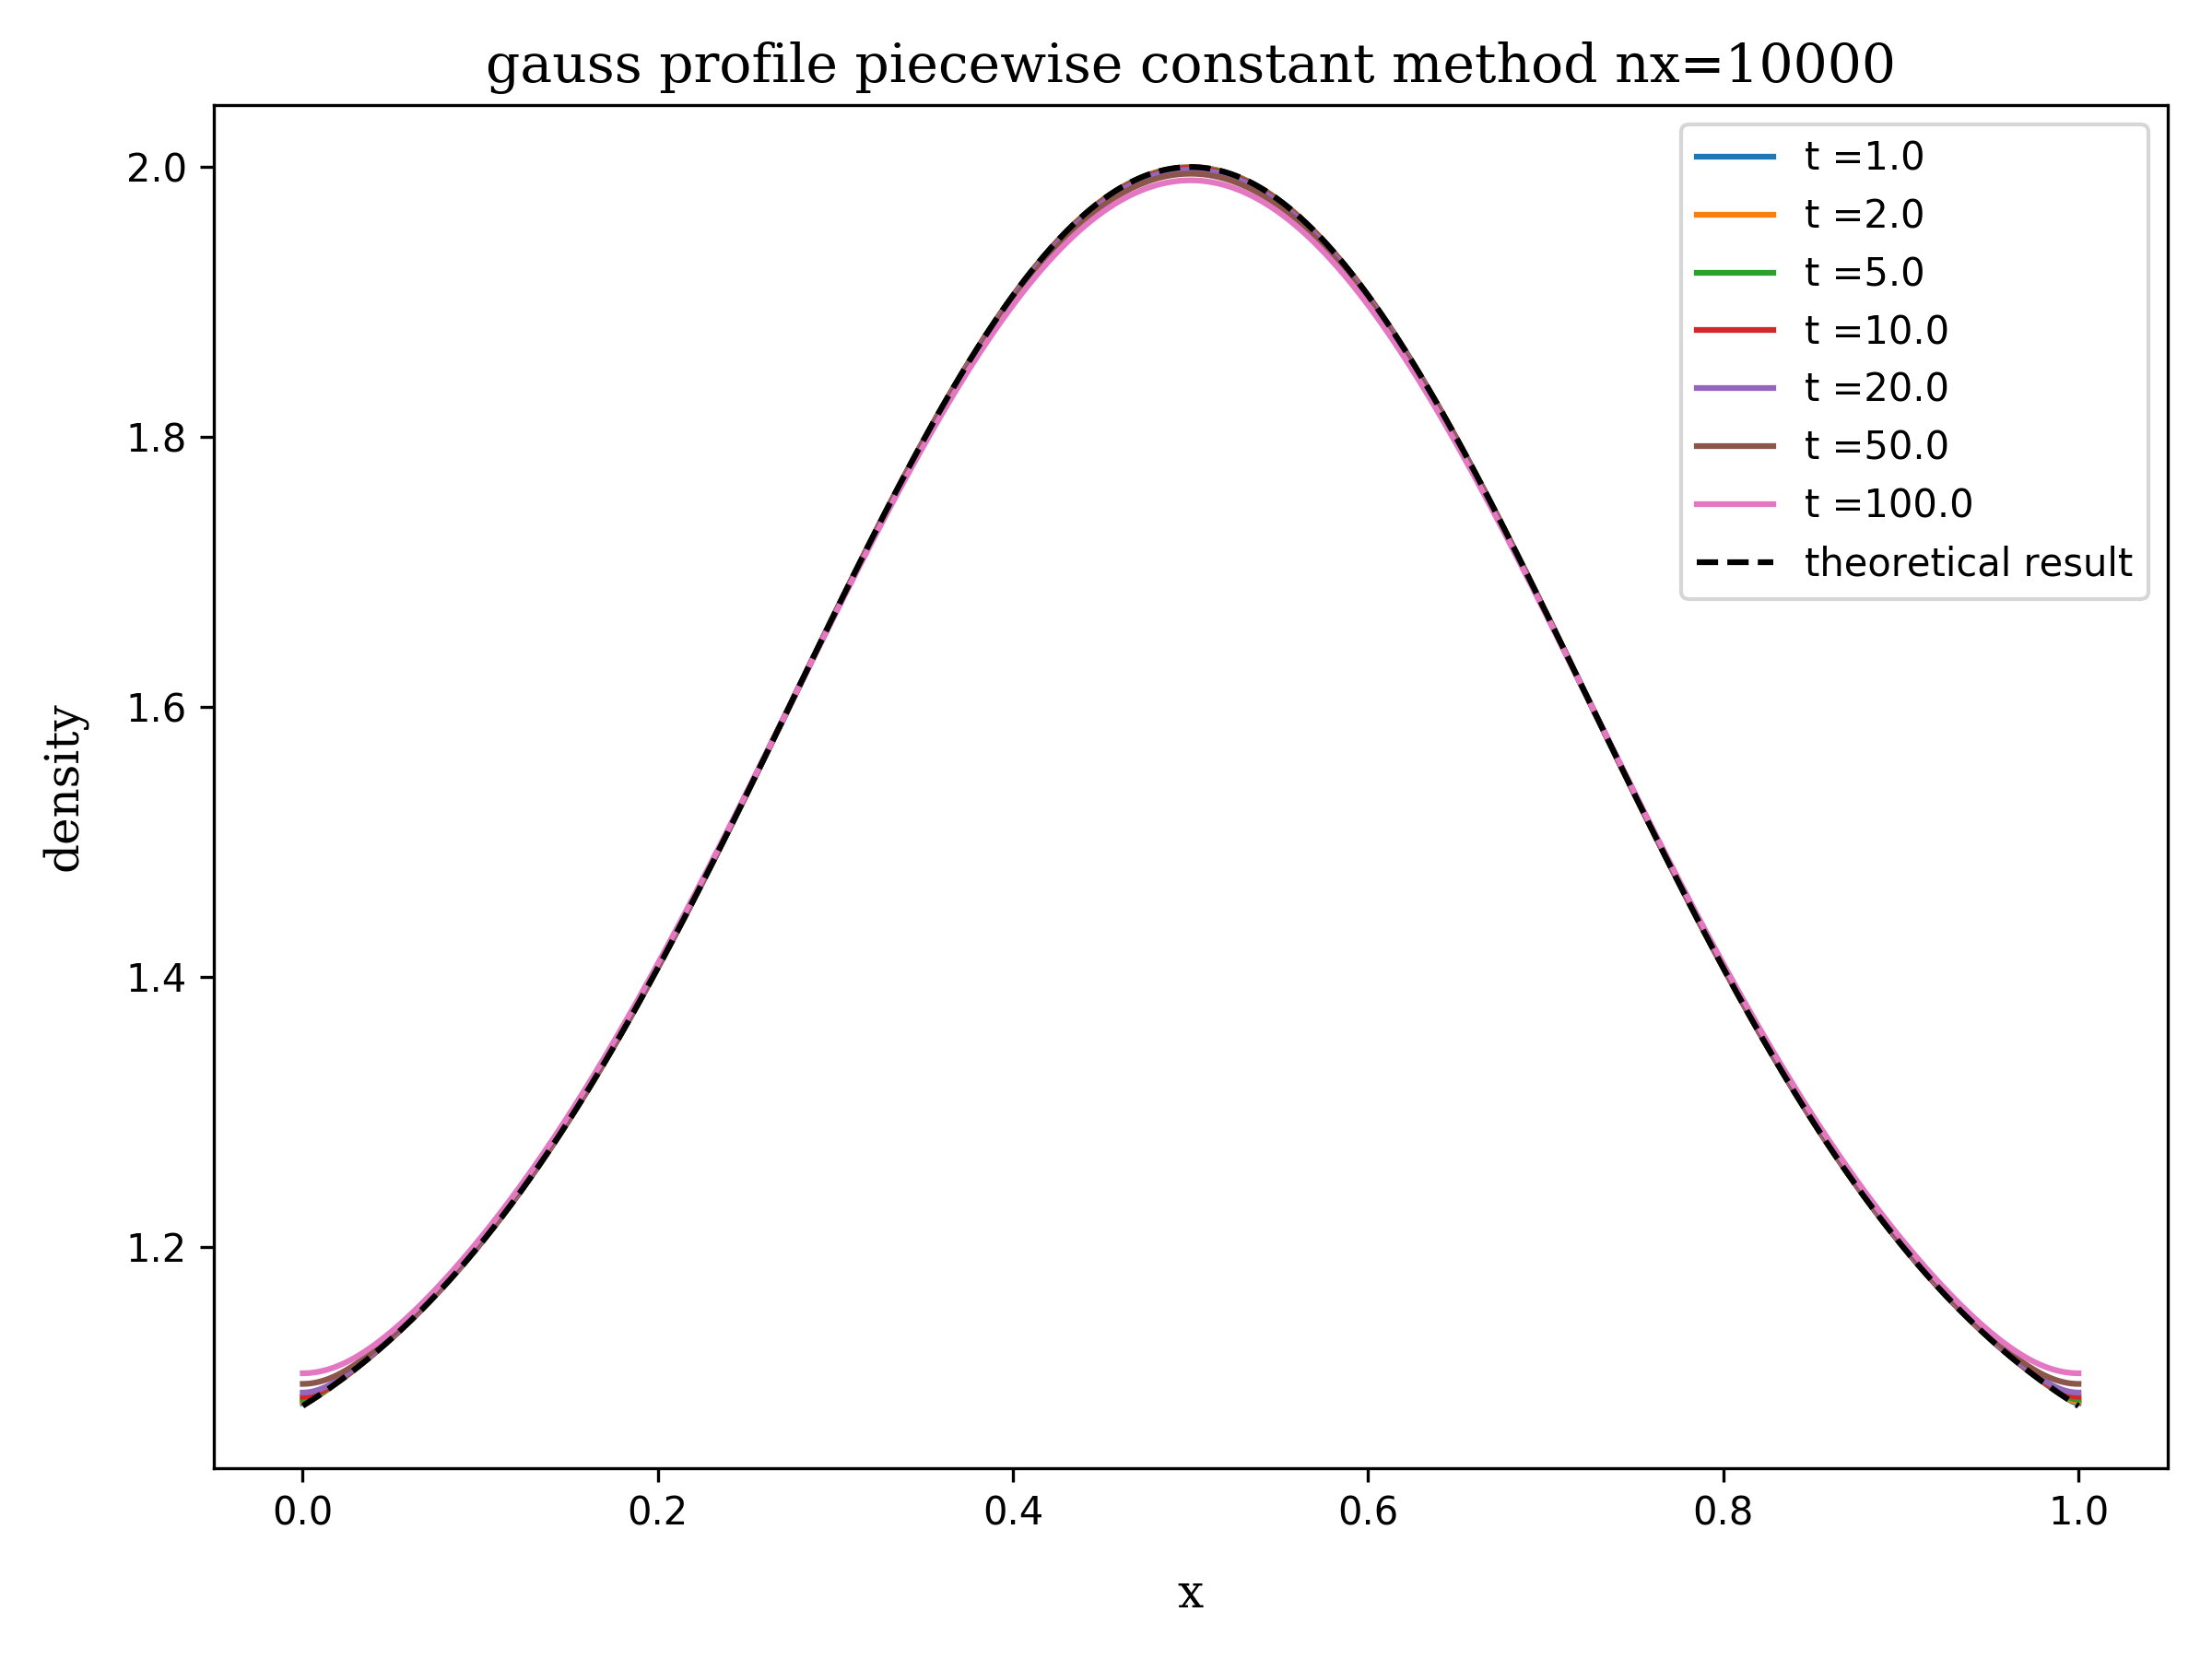
\includegraphics[height=.33\textheight]{../results/1D/pwconst/nx=10000/plot_advection_gauss_pwconst_nx=10000.png}
	\end{columns}
\end{frame}




\section{Piecewise Linear Method}

\begin{frame}
	\frametitle{Piecewise Linear Method}

		Assume that the state in the cell is piecewise linear with some slope $s$. This gives a second-order accurate method.
		\begin{align*}
			\text{For } && x_{i-\half} < x_i < x_{i+\half}: &
			\quad \rho(x, t=t_n) = \rho_i^n + s_i^n(x - x_i)\\[.5em]			
			\text{For }&& t_n < t < t_{n+1}: &\quad \rho(x, t) = \rho_i^n +s_i^n(x -[x_i + u (t - t_n)])
		\end{align*}
%		
		The flux over the interface is then
%
		\begin{align*}
			f_{i-\half}(t) 	&= u \rho(x = x_{i-\half}, t)\\
						&= u \rho_{i-1} +  u s_i^n(\nicefrac{\Delta x}{2} - u(t-t_n))
		\end{align*}
%
		Finally averaging the fluxes over a time step gives:
		\begin{align*}
			\rho_i^{n+1} = \rho_i^n - \frac{u \Delta t}{\Delta x} ( \rho_i ^n - \rho_{i-1}^n) - \frac{u \Delta t}{\Delta x} \frac{1}{2} (s_i^n - s_{i-1}^n)(\Delta x - u\Delta t)
		\end{align*}
		
		Choice of slope: $s_i^n = \frac{\rho_{i+1}^n - \rho_i^n}{\Delta x}$ ( Lax-Wendroff method )

\end{frame}









\begin{frame}
	\vspace{10pt}
	\begin{columns}
		\column{.33\textwidth}
			\centering
			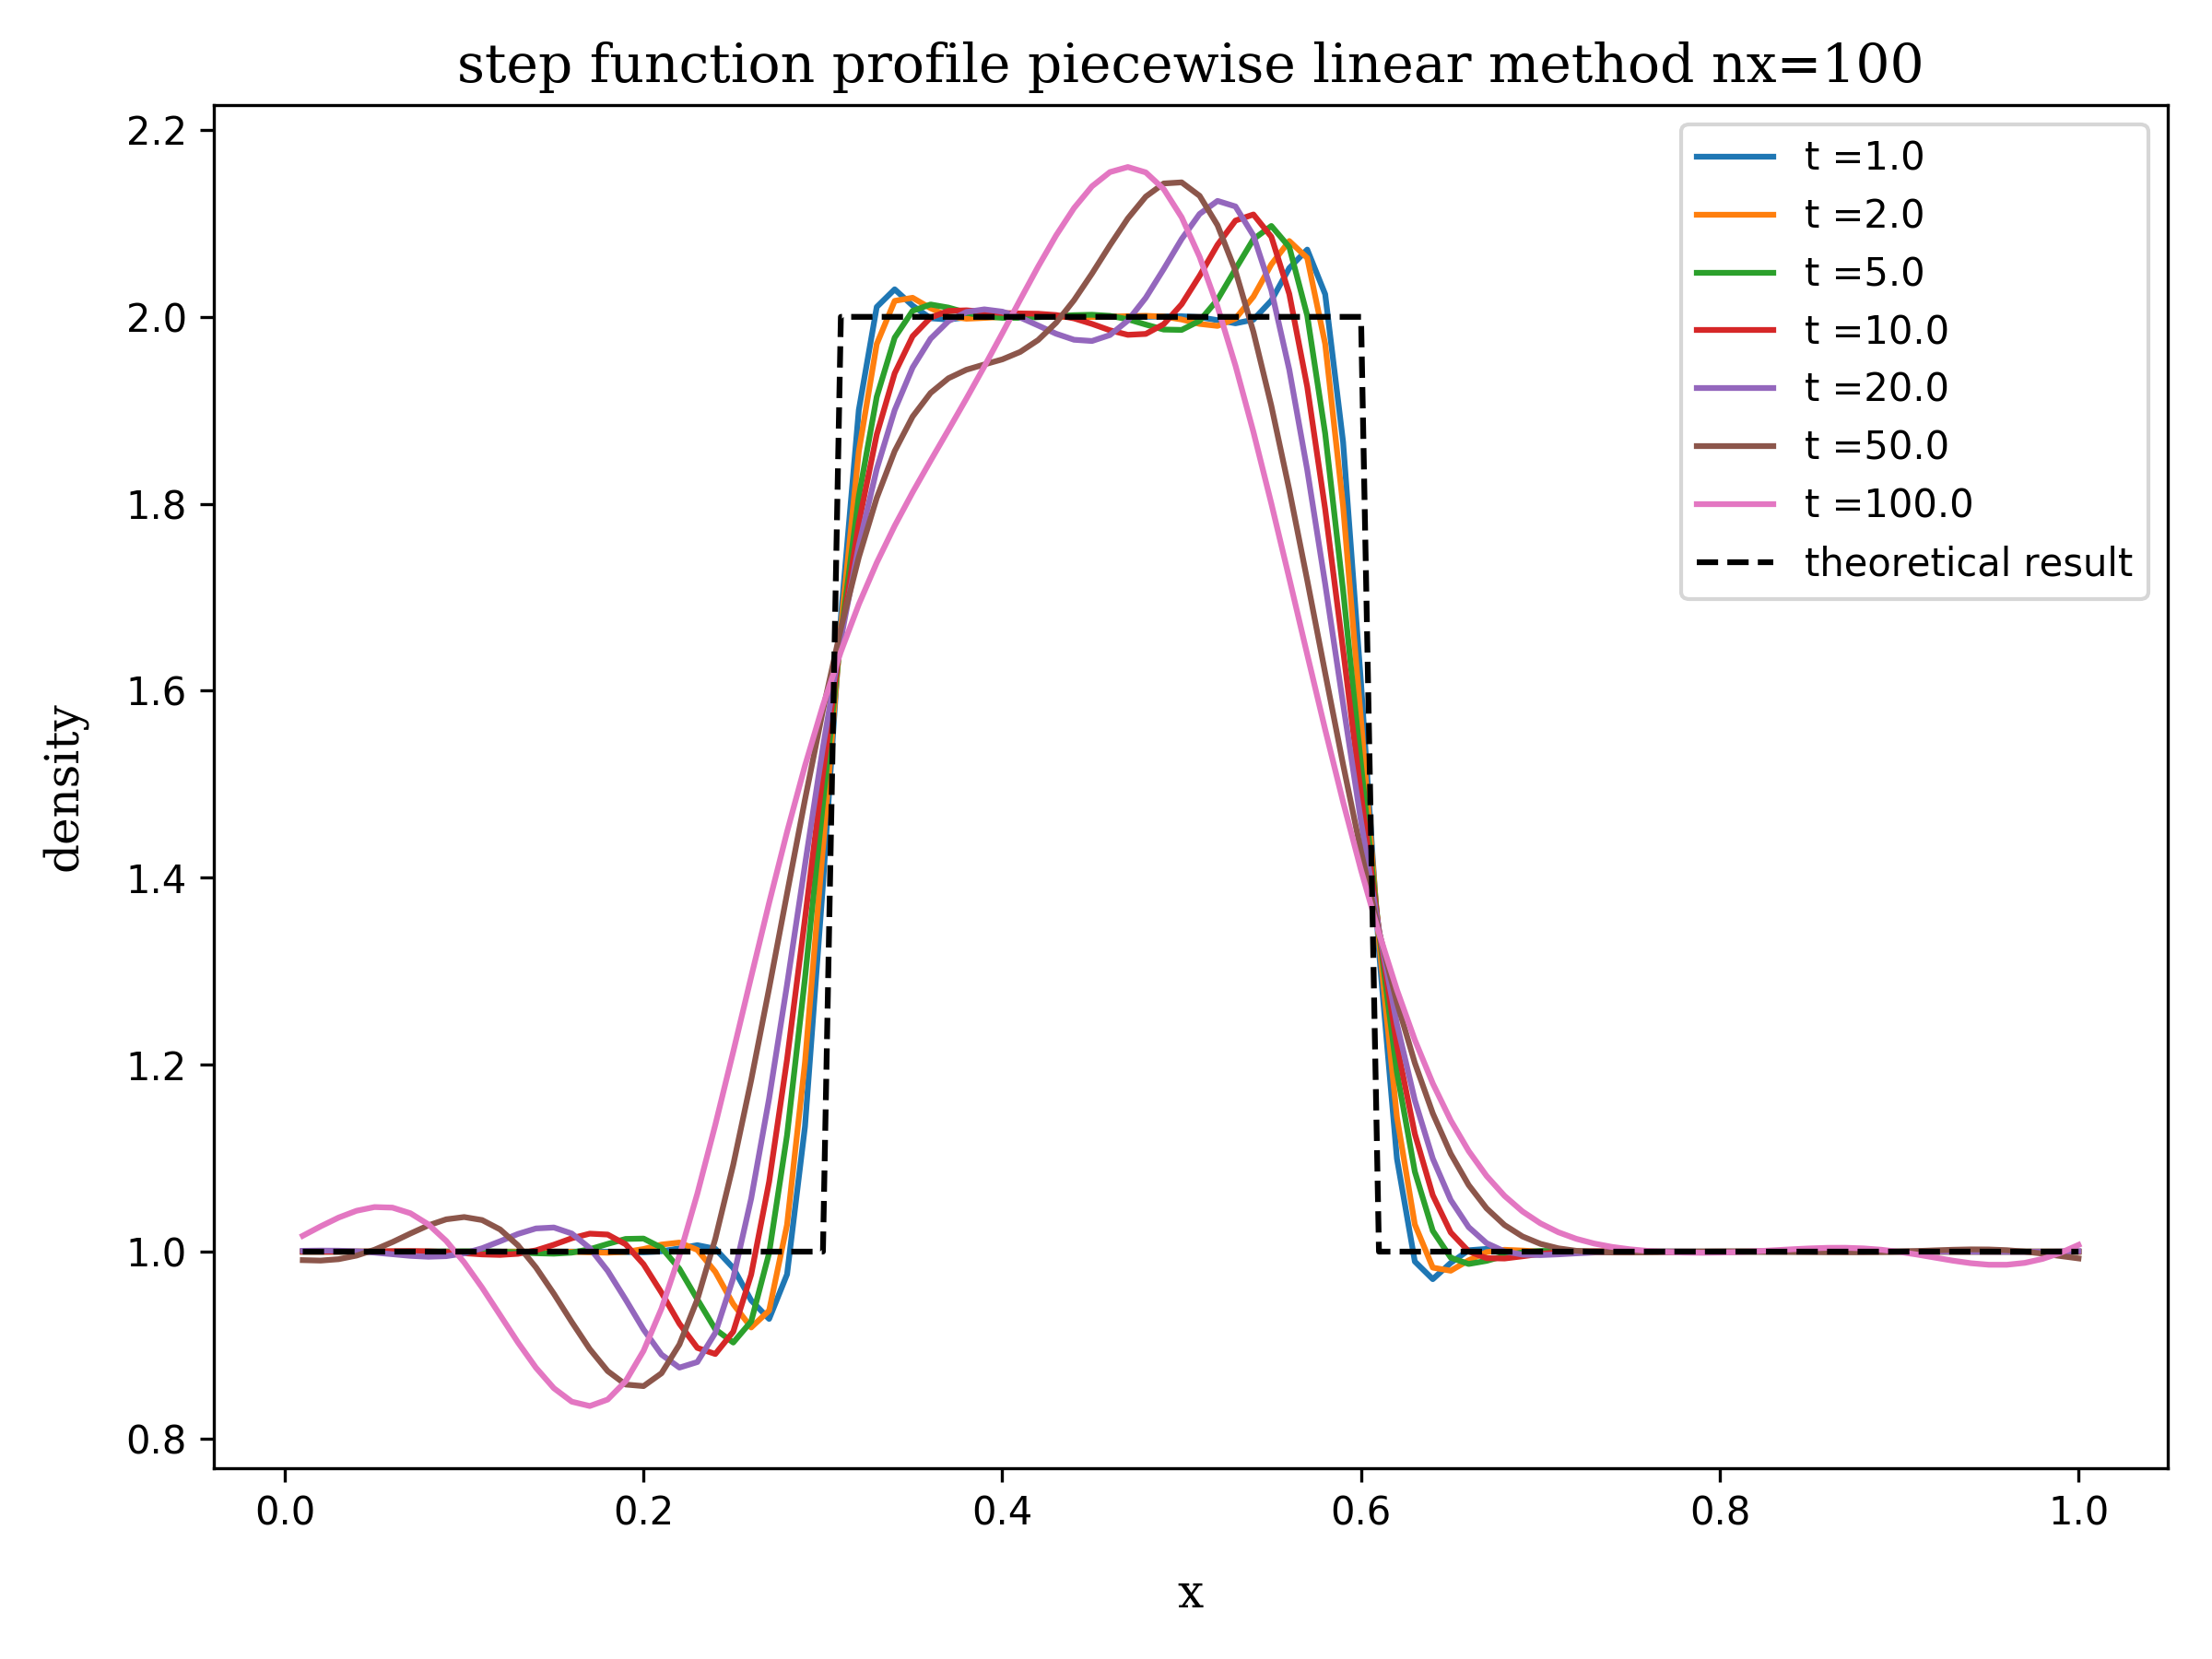
\includegraphics[height=.33\textheight]{../results/1D/pwlin/nx=100/plot_advection_step_function_pwlin_nx=100.png}\\
			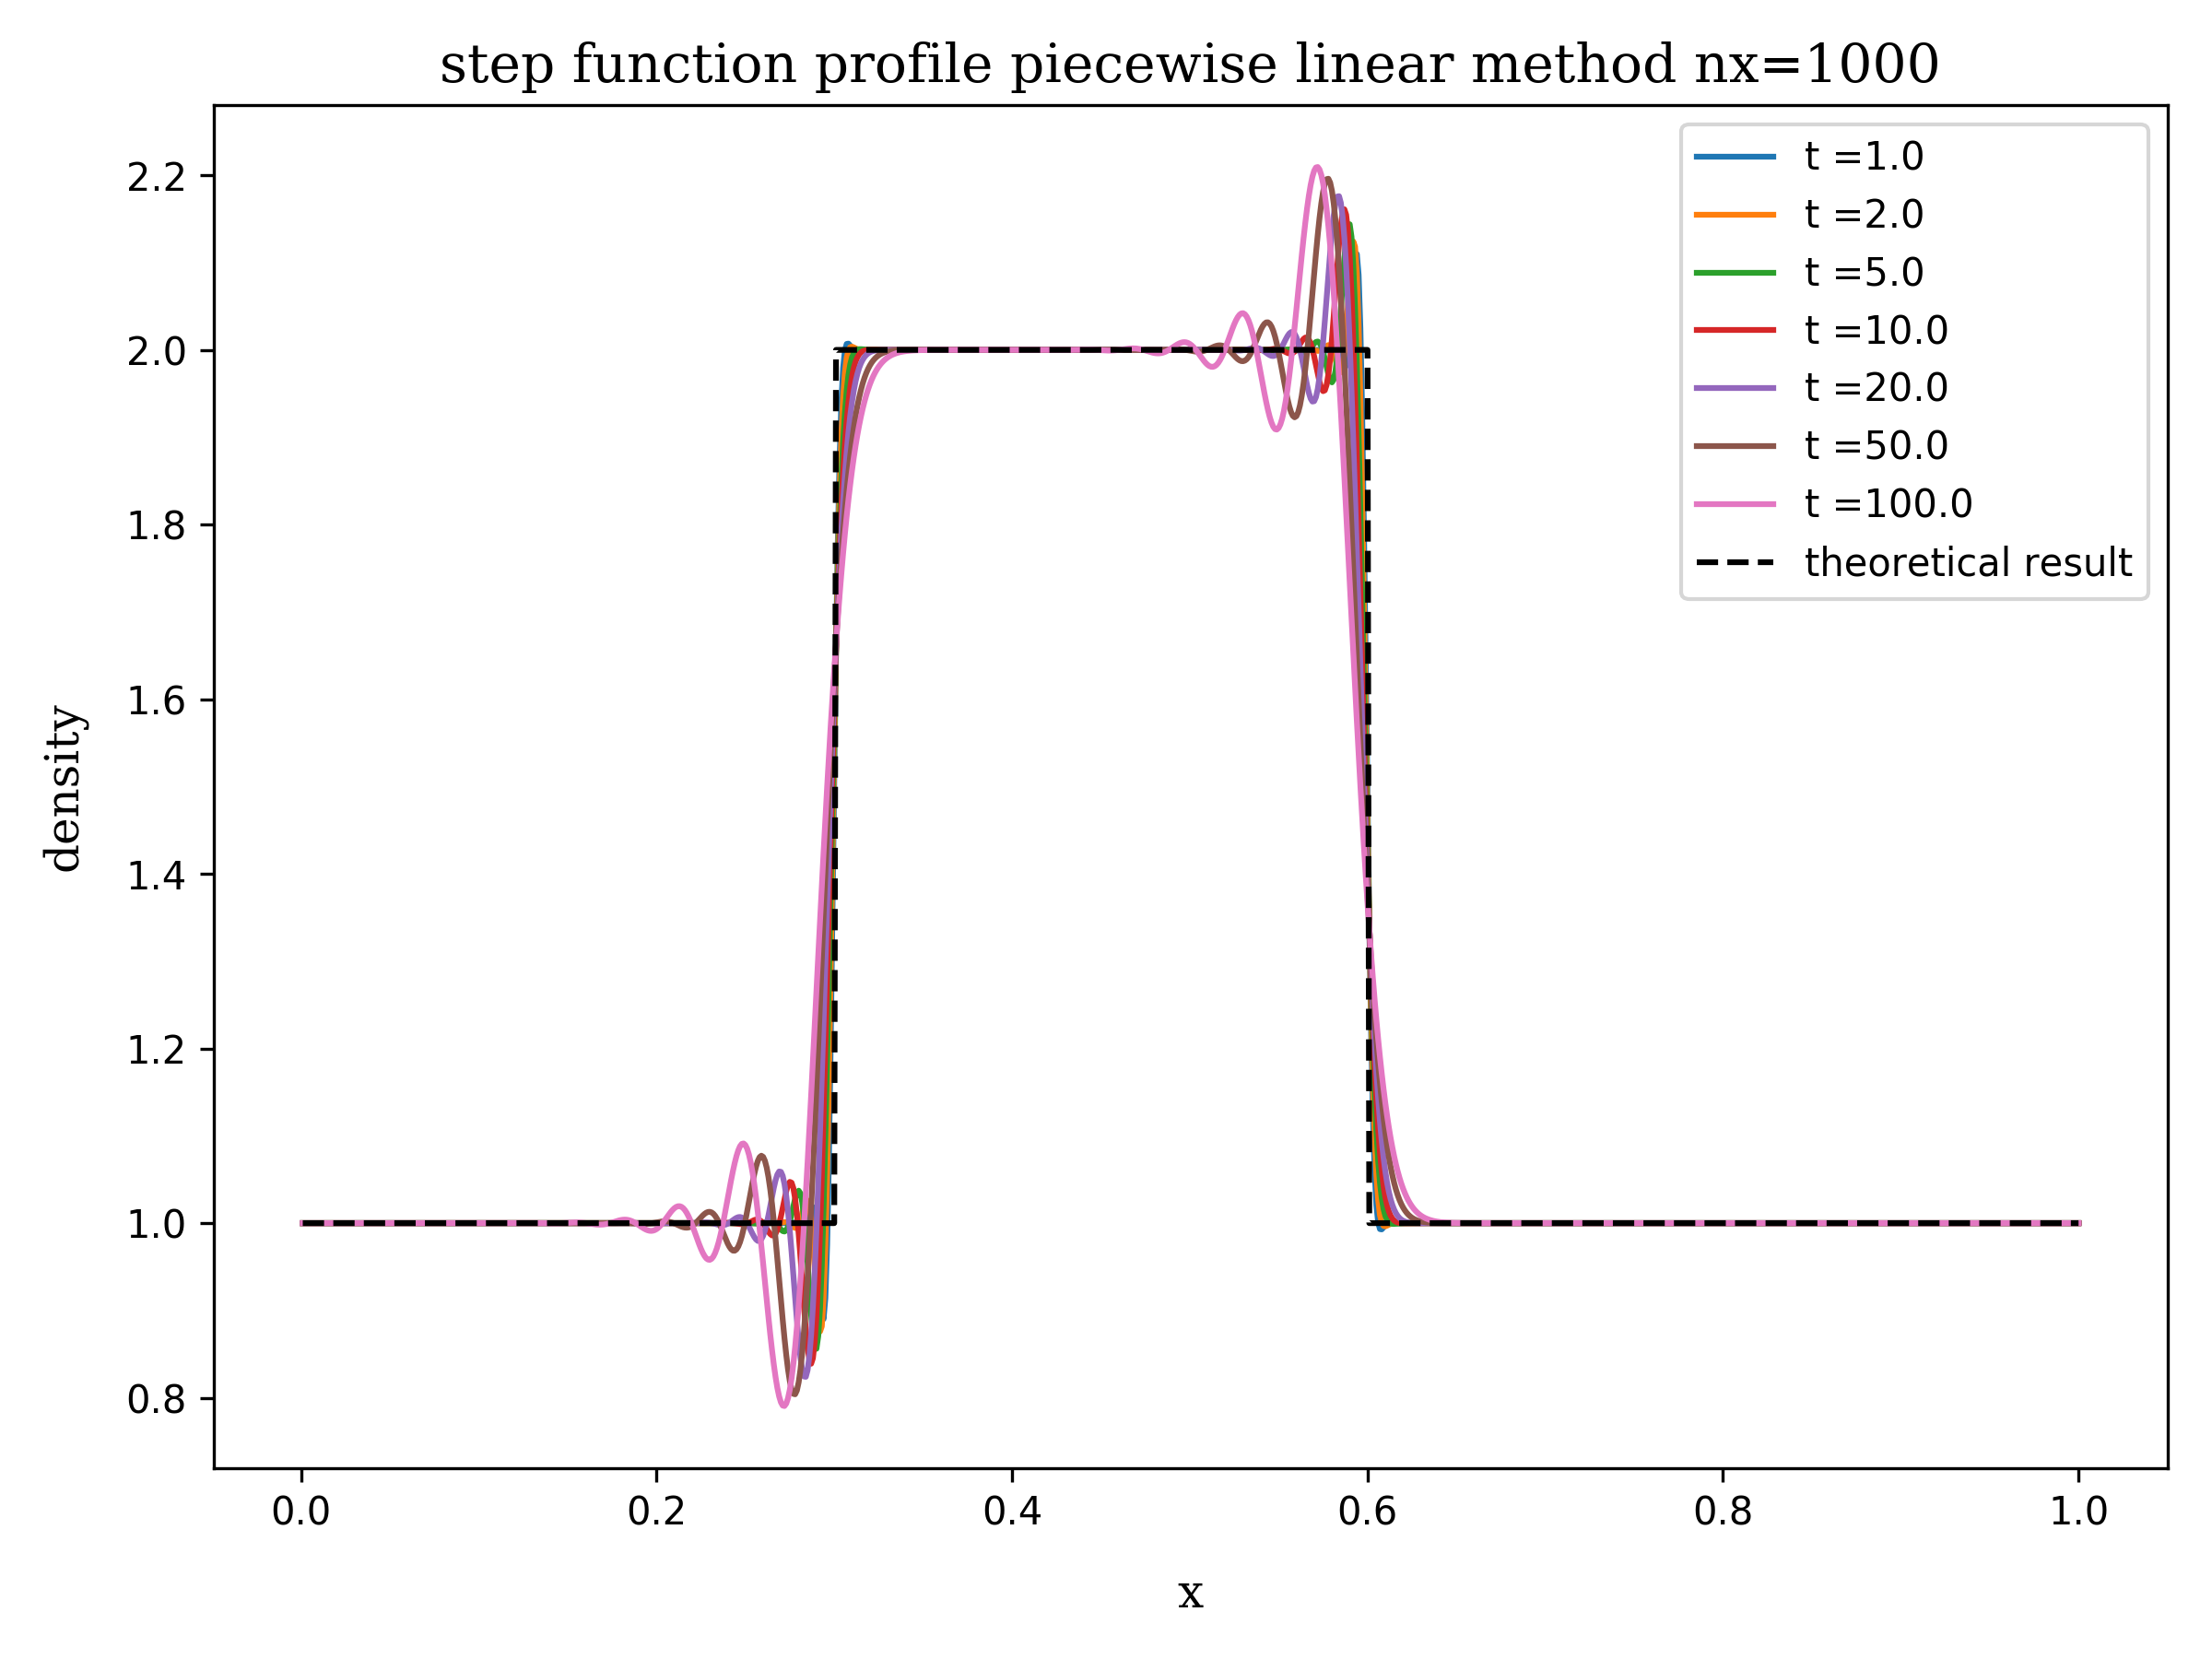
\includegraphics[height=.33\textheight]{../results/1D/pwlin/nx=1000/plot_advection_step_function_pwlin_nx=1000.png}\\
			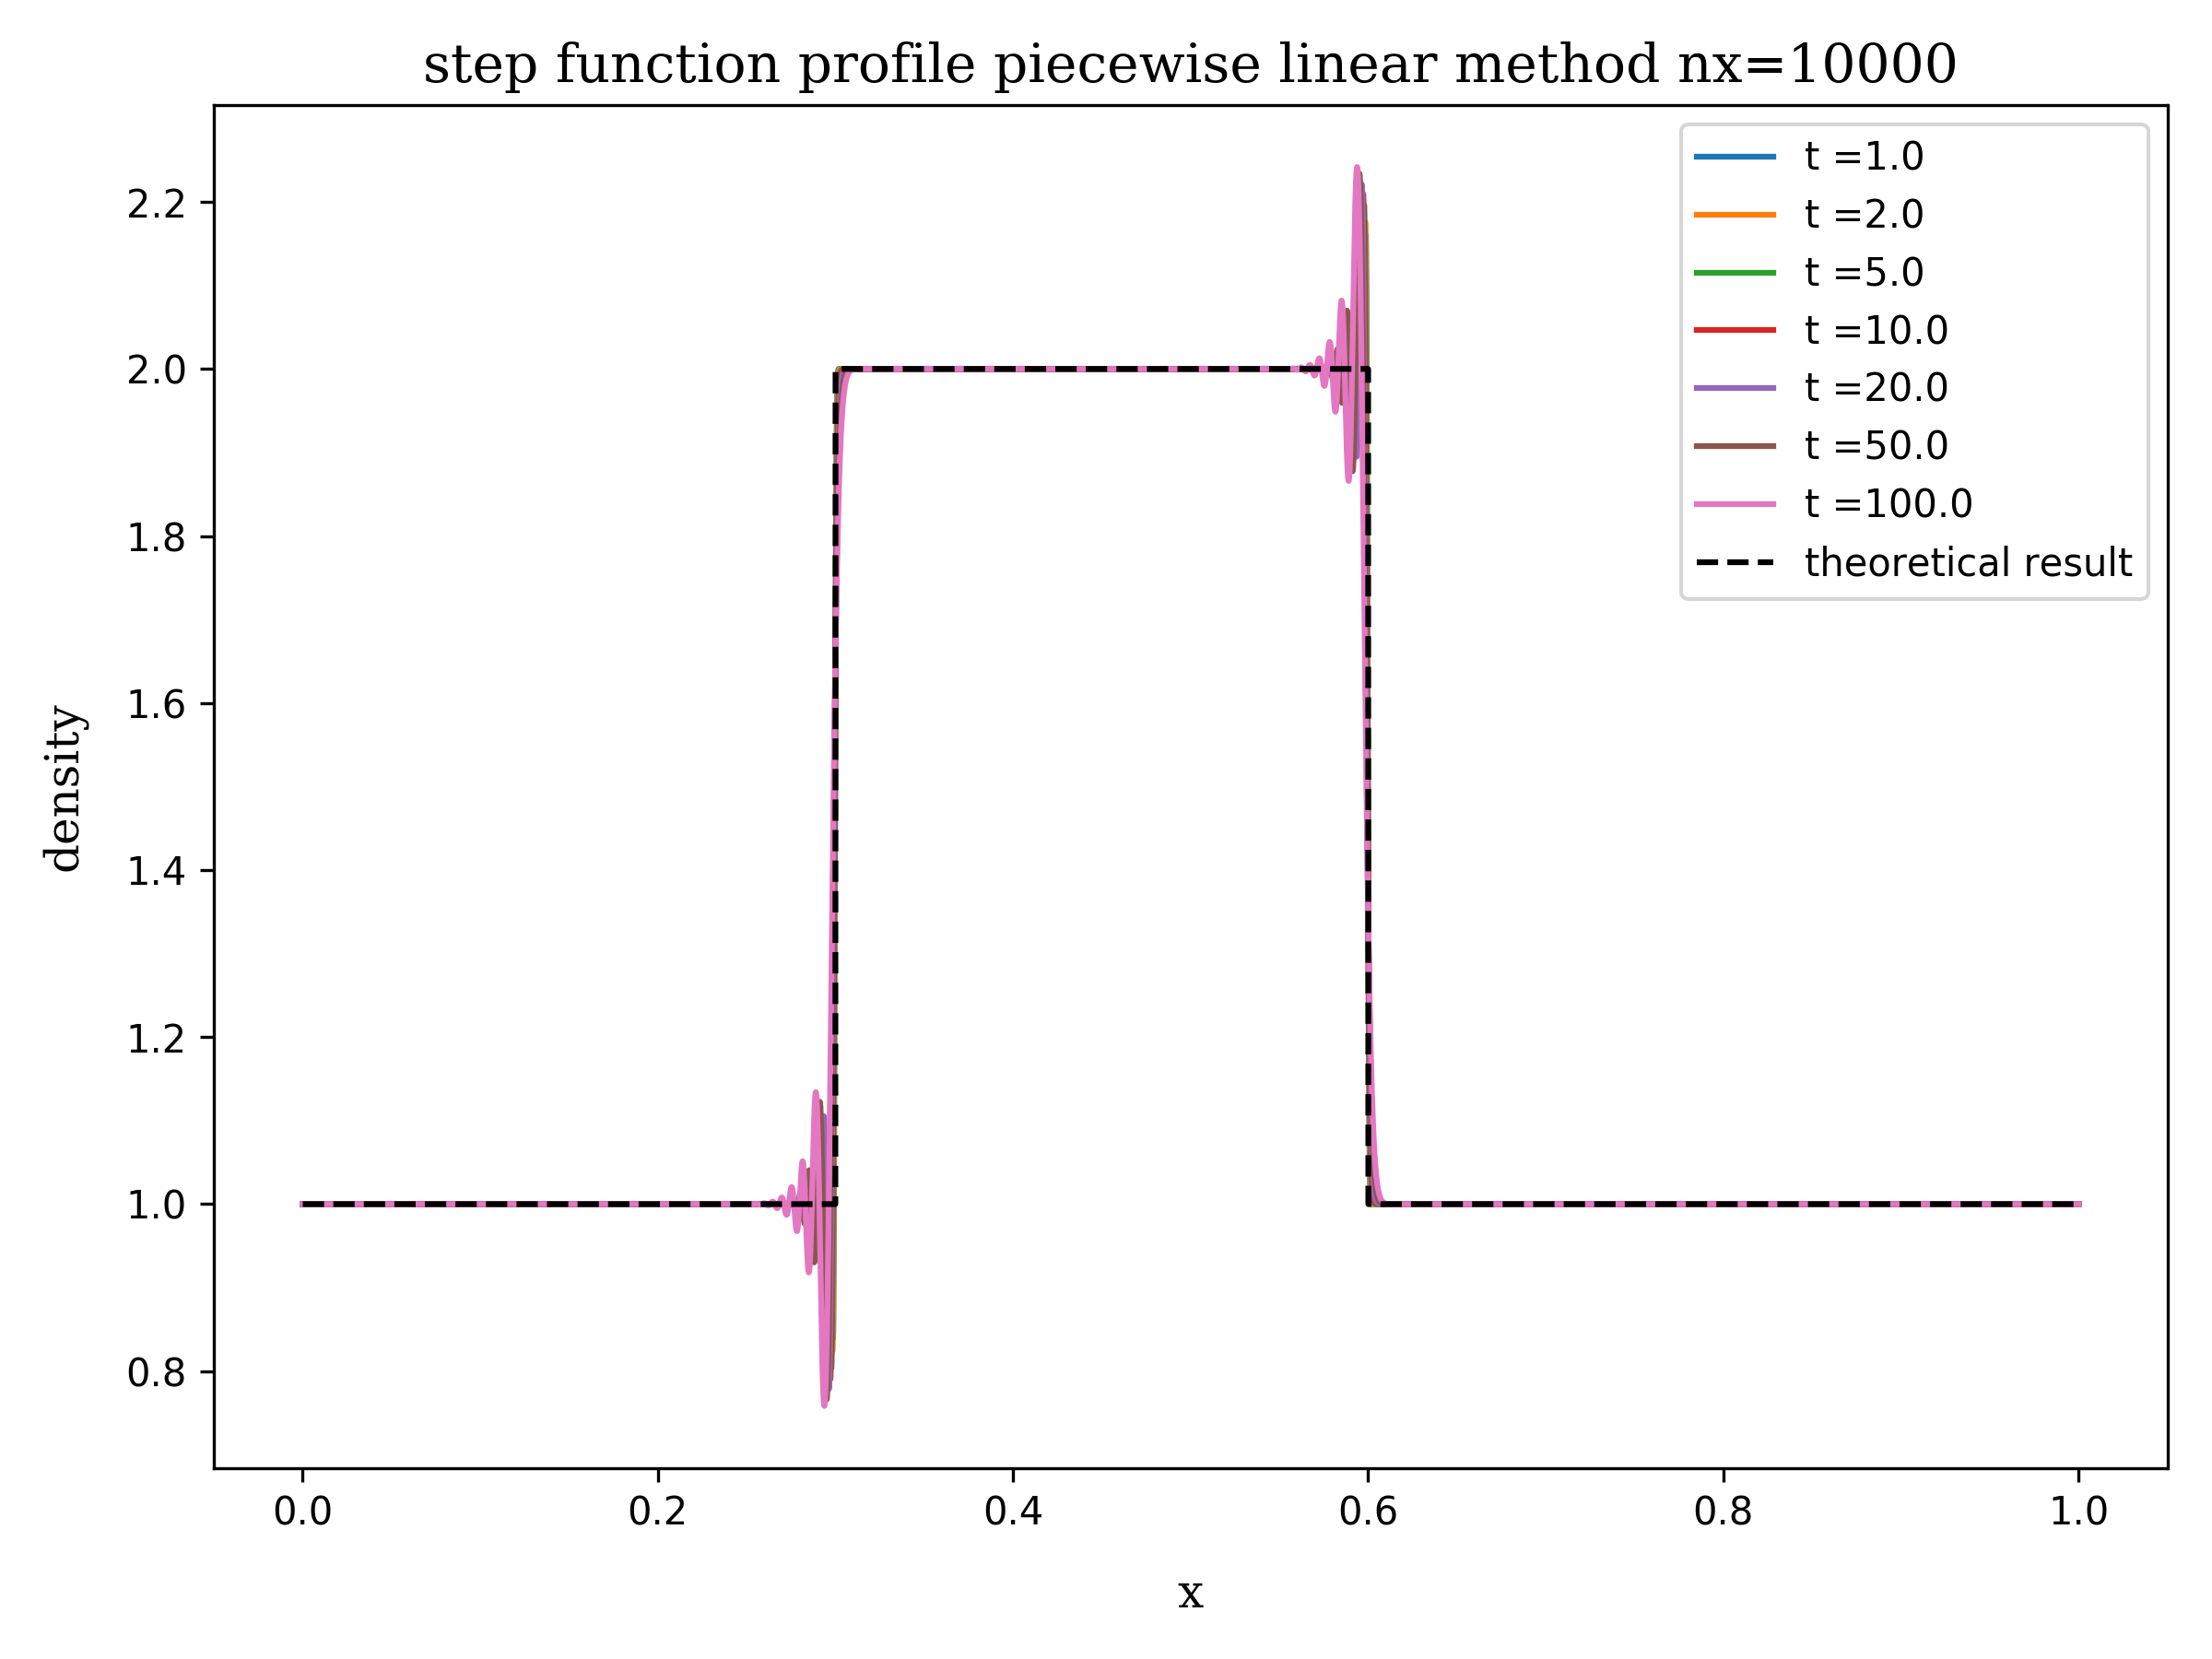
\includegraphics[height=.33\textheight]{../results/1D/pwlin/nx=10000/plot_advection_step_function_pwlin_nx=10000.png}
		\column{.33\textwidth}
			\centering
			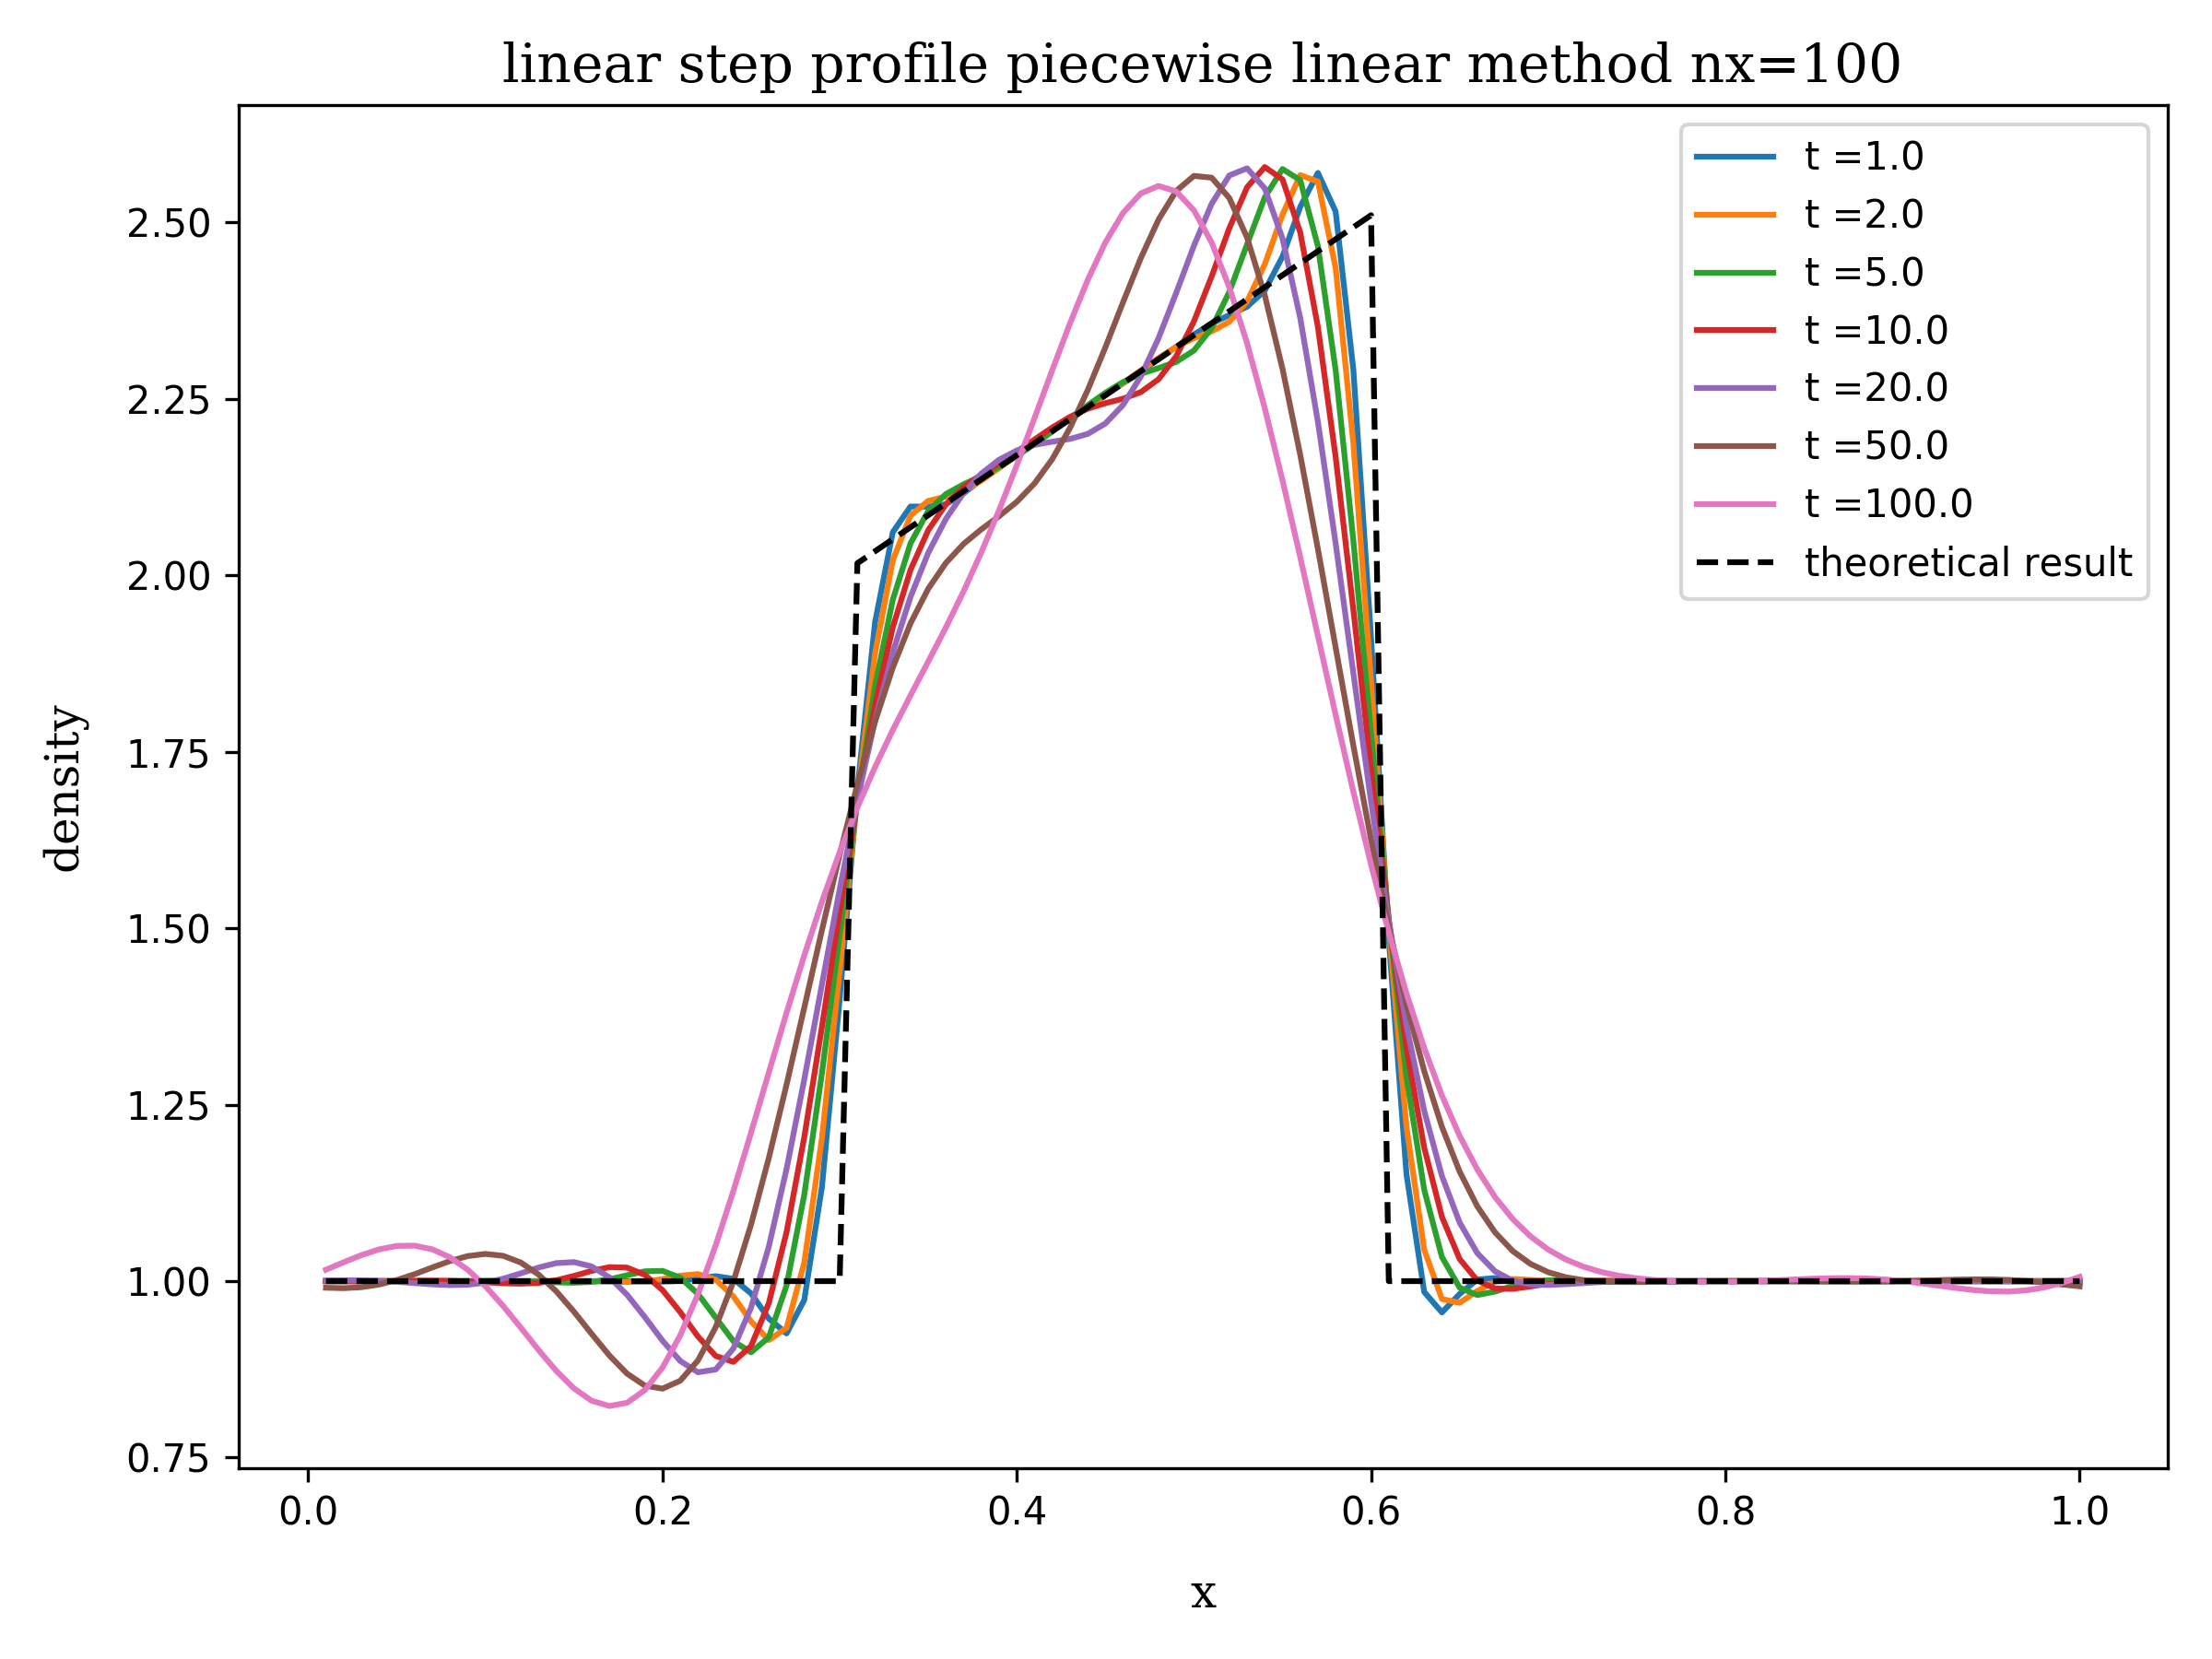
\includegraphics[height=.33\textheight]{../results/1D/pwlin/nx=100/plot_advection_linear_step_pwlin_nx=100.png}\\
			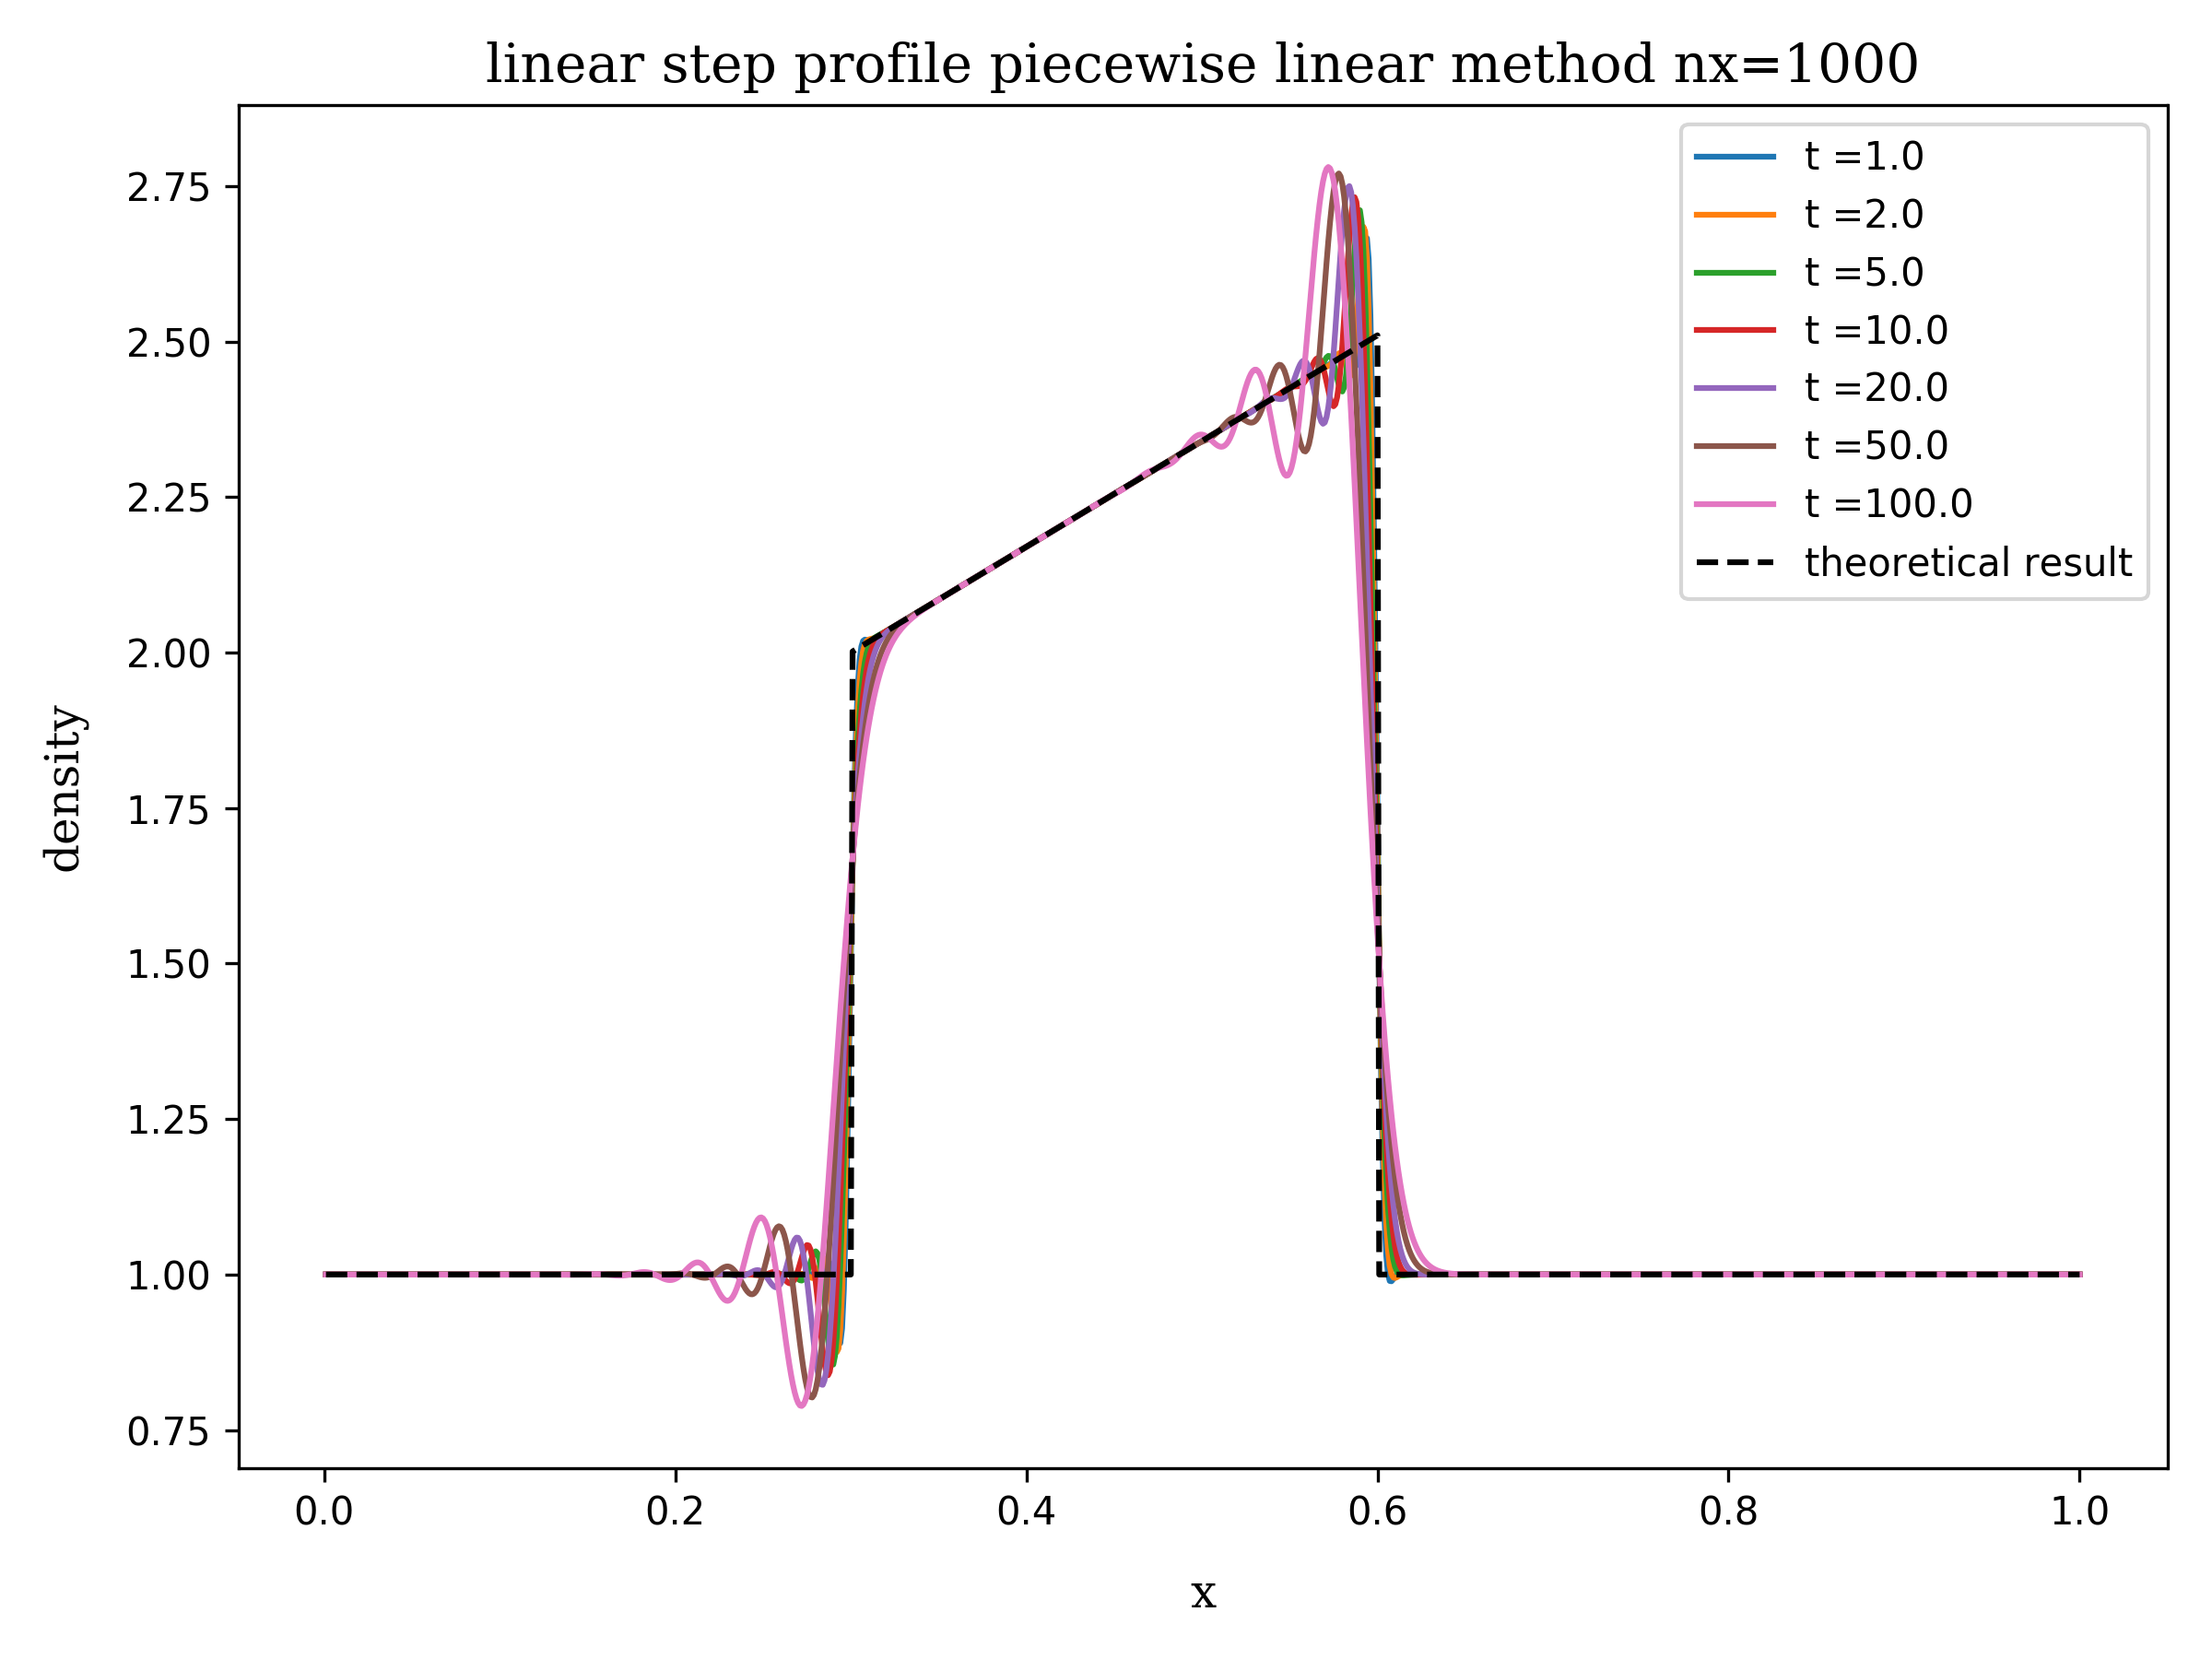
\includegraphics[height=.33\textheight]{../results/1D/pwlin/nx=1000/plot_advection_linear_step_pwlin_nx=1000.png}\\
			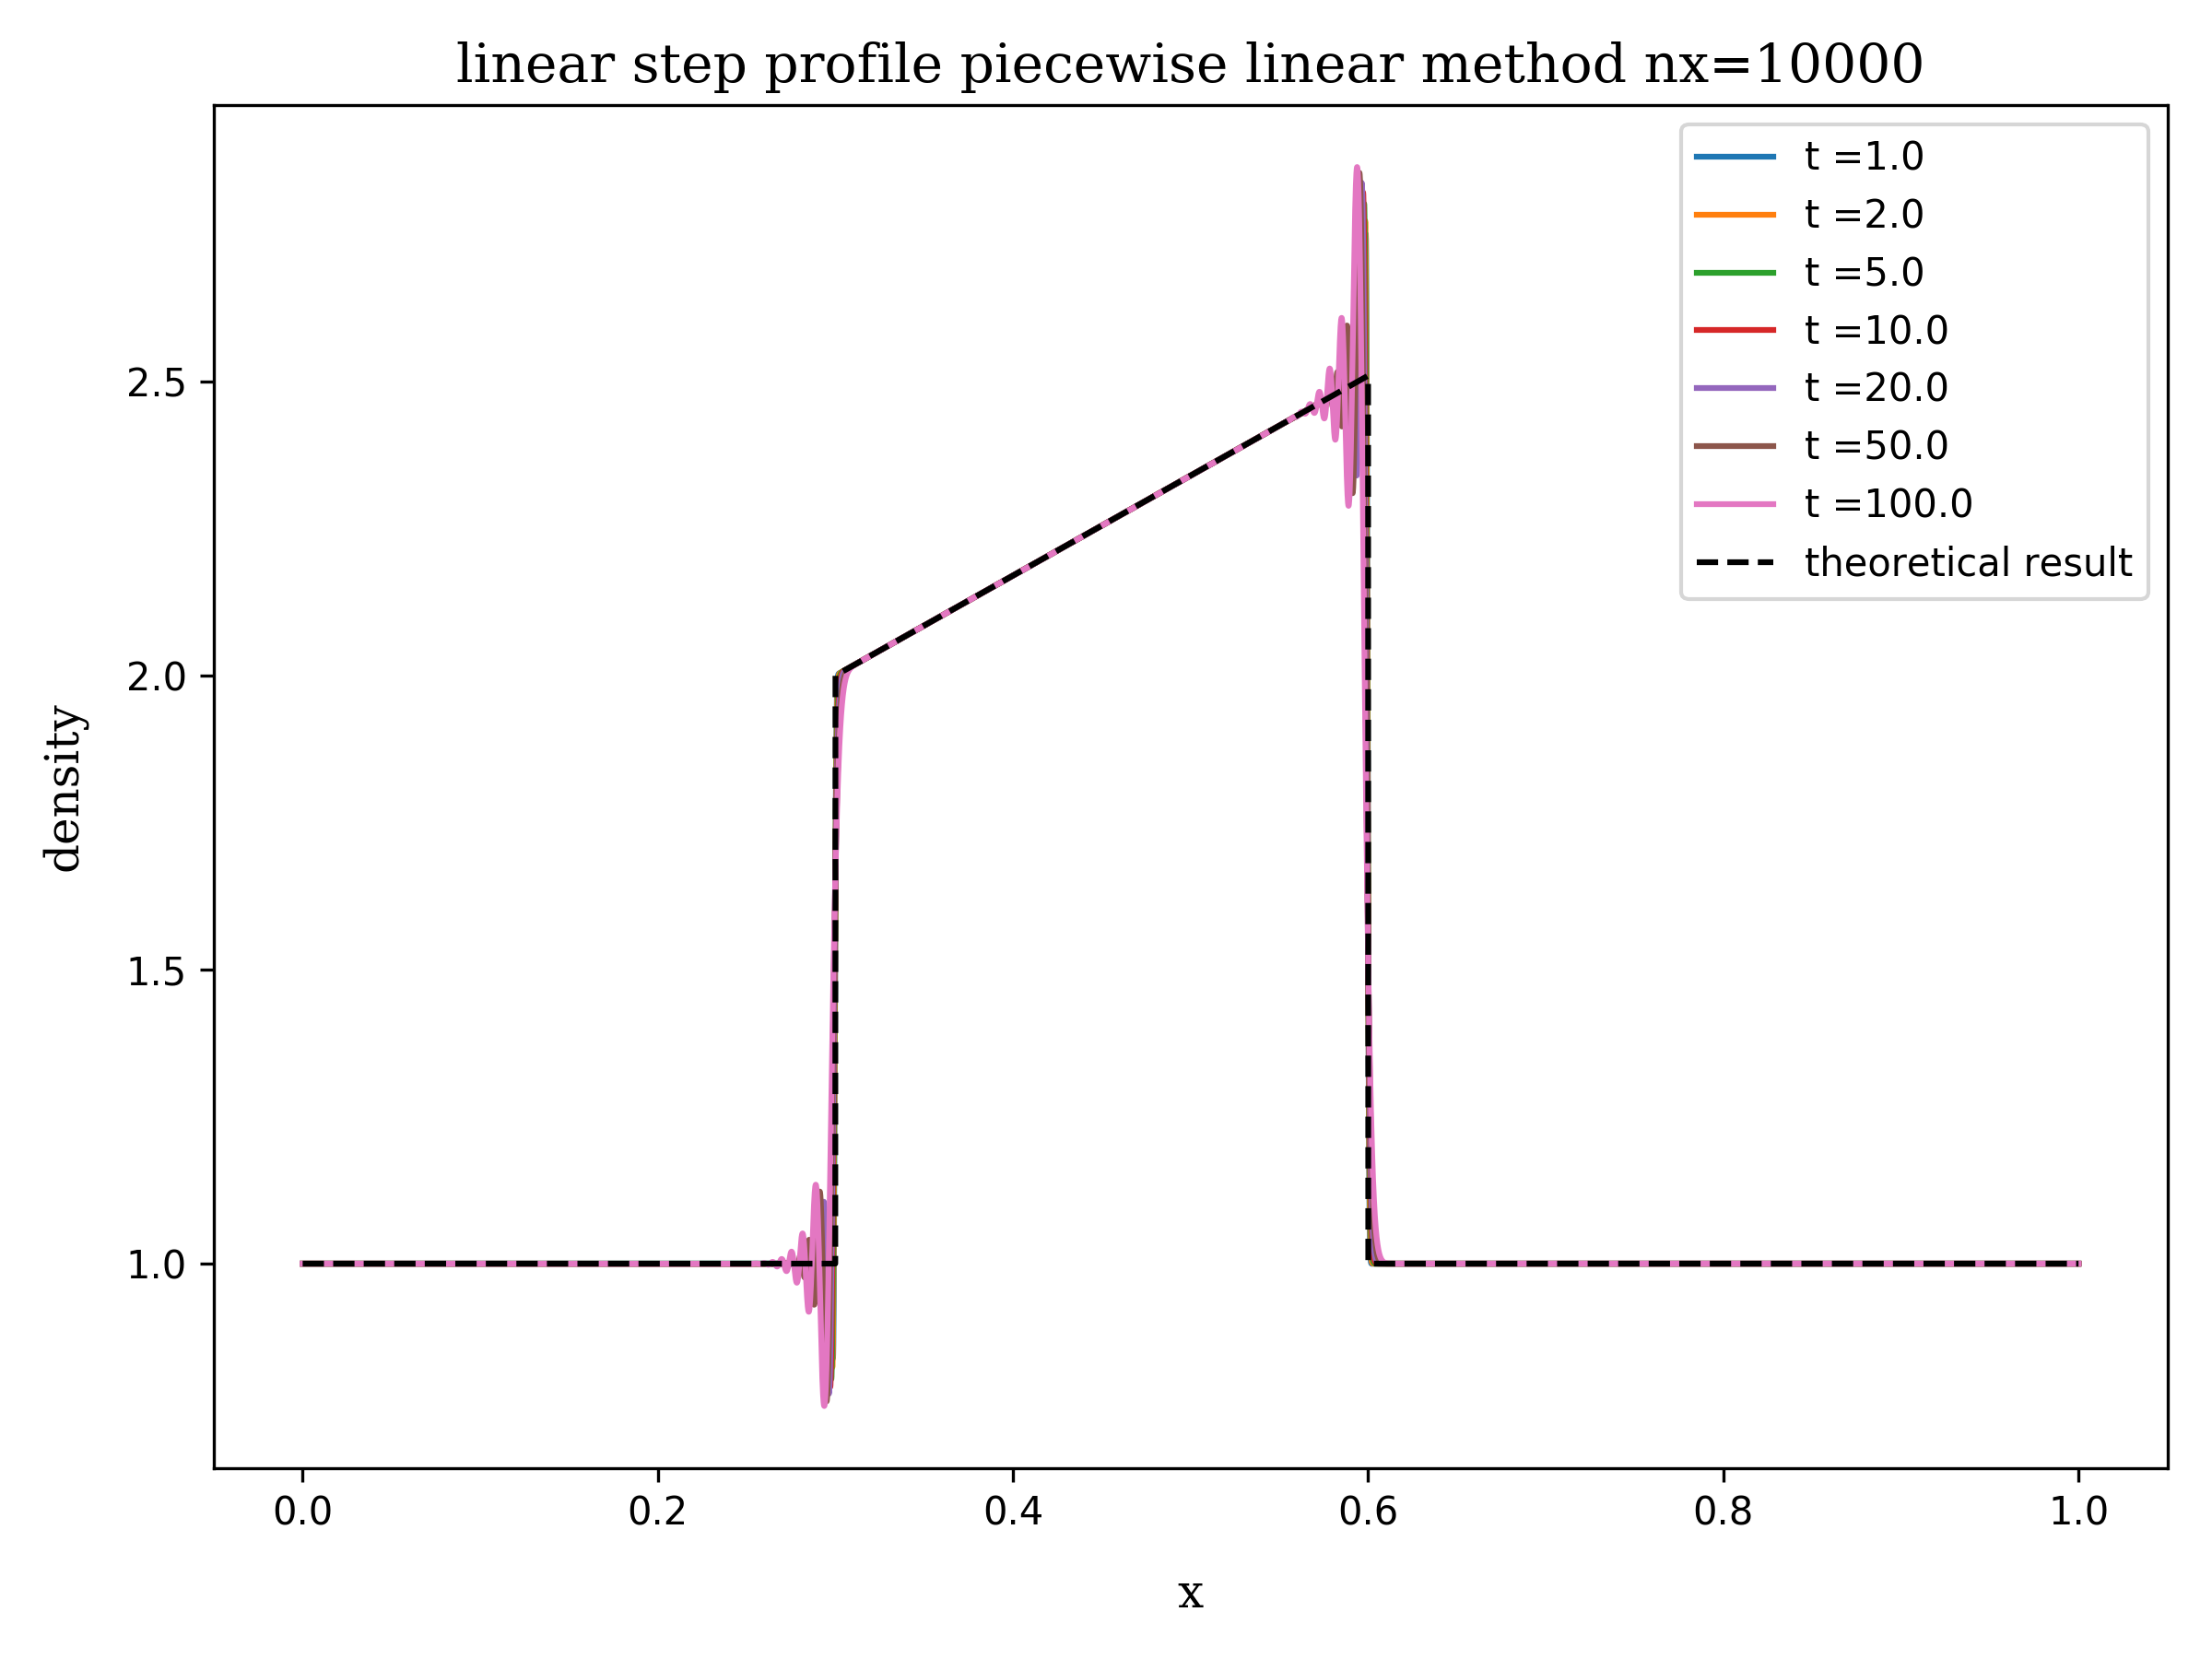
\includegraphics[height=.33\textheight]{../results/1D/pwlin/nx=10000/plot_advection_linear_step_pwlin_nx=10000.png}
		\column{.33\textwidth}
			\centering
			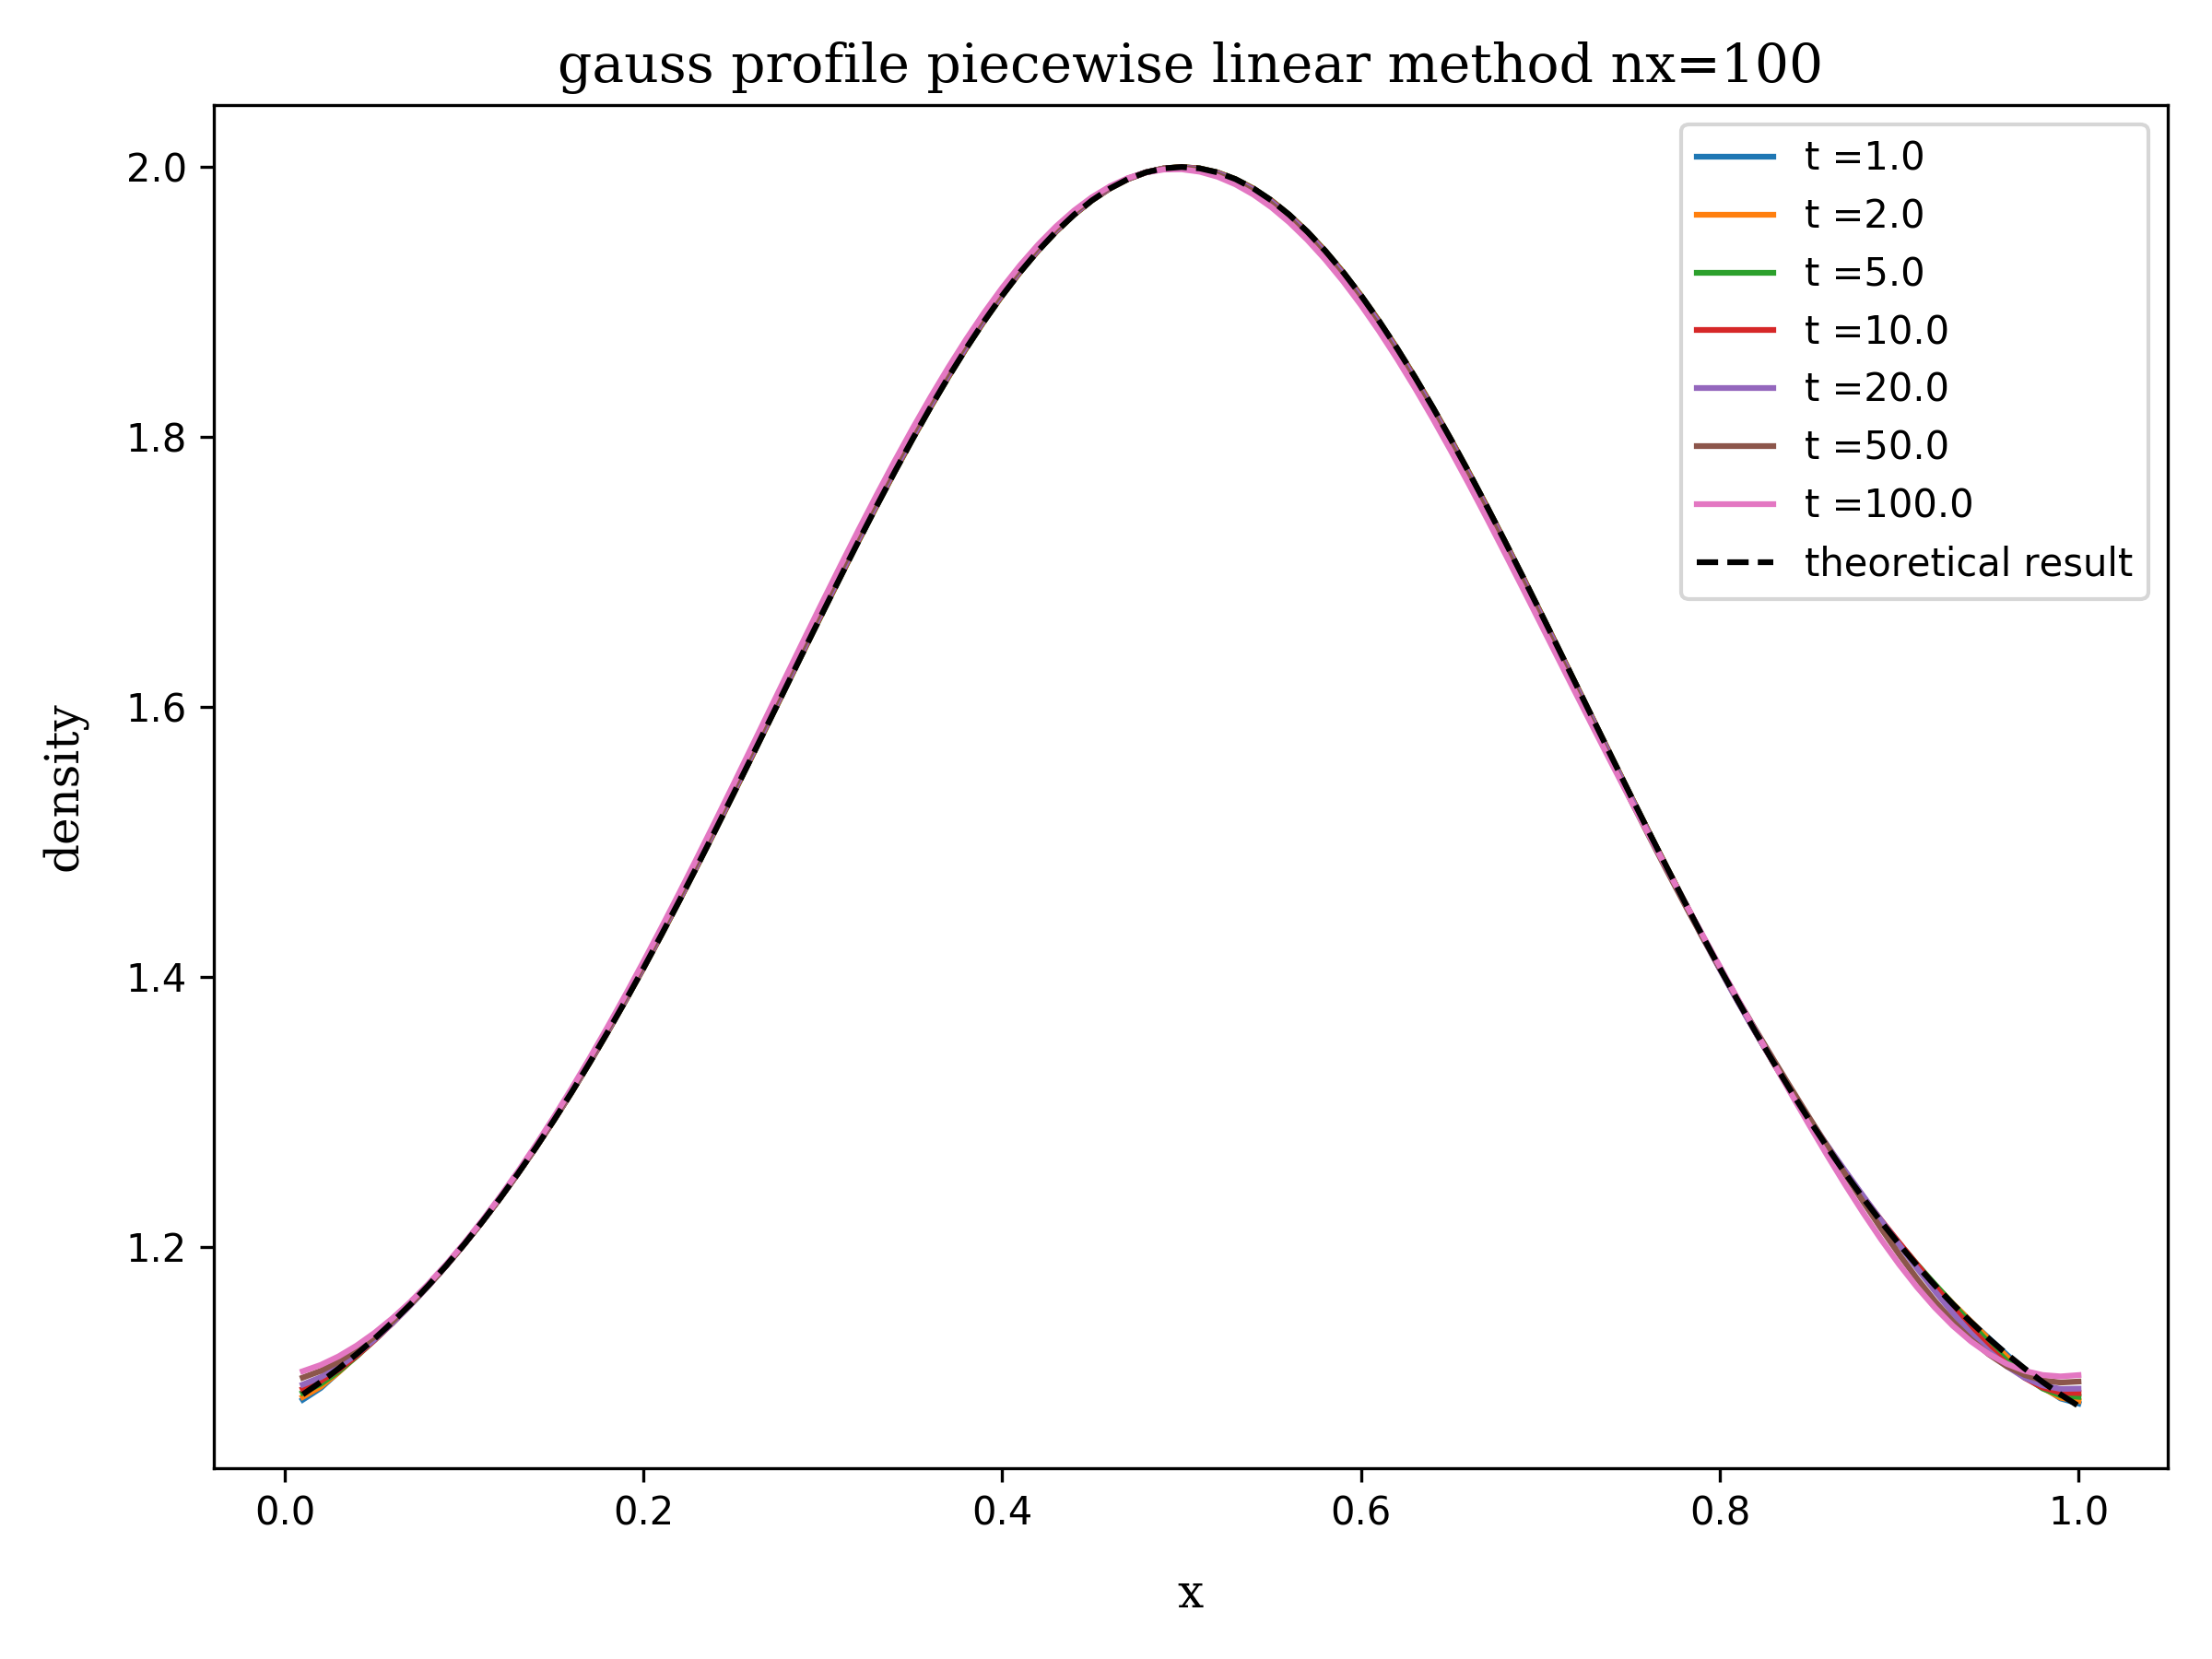
\includegraphics[height=.33\textheight]{../results/1D/pwlin/nx=100/plot_advection_gauss_pwlin_nx=100.png}\\
			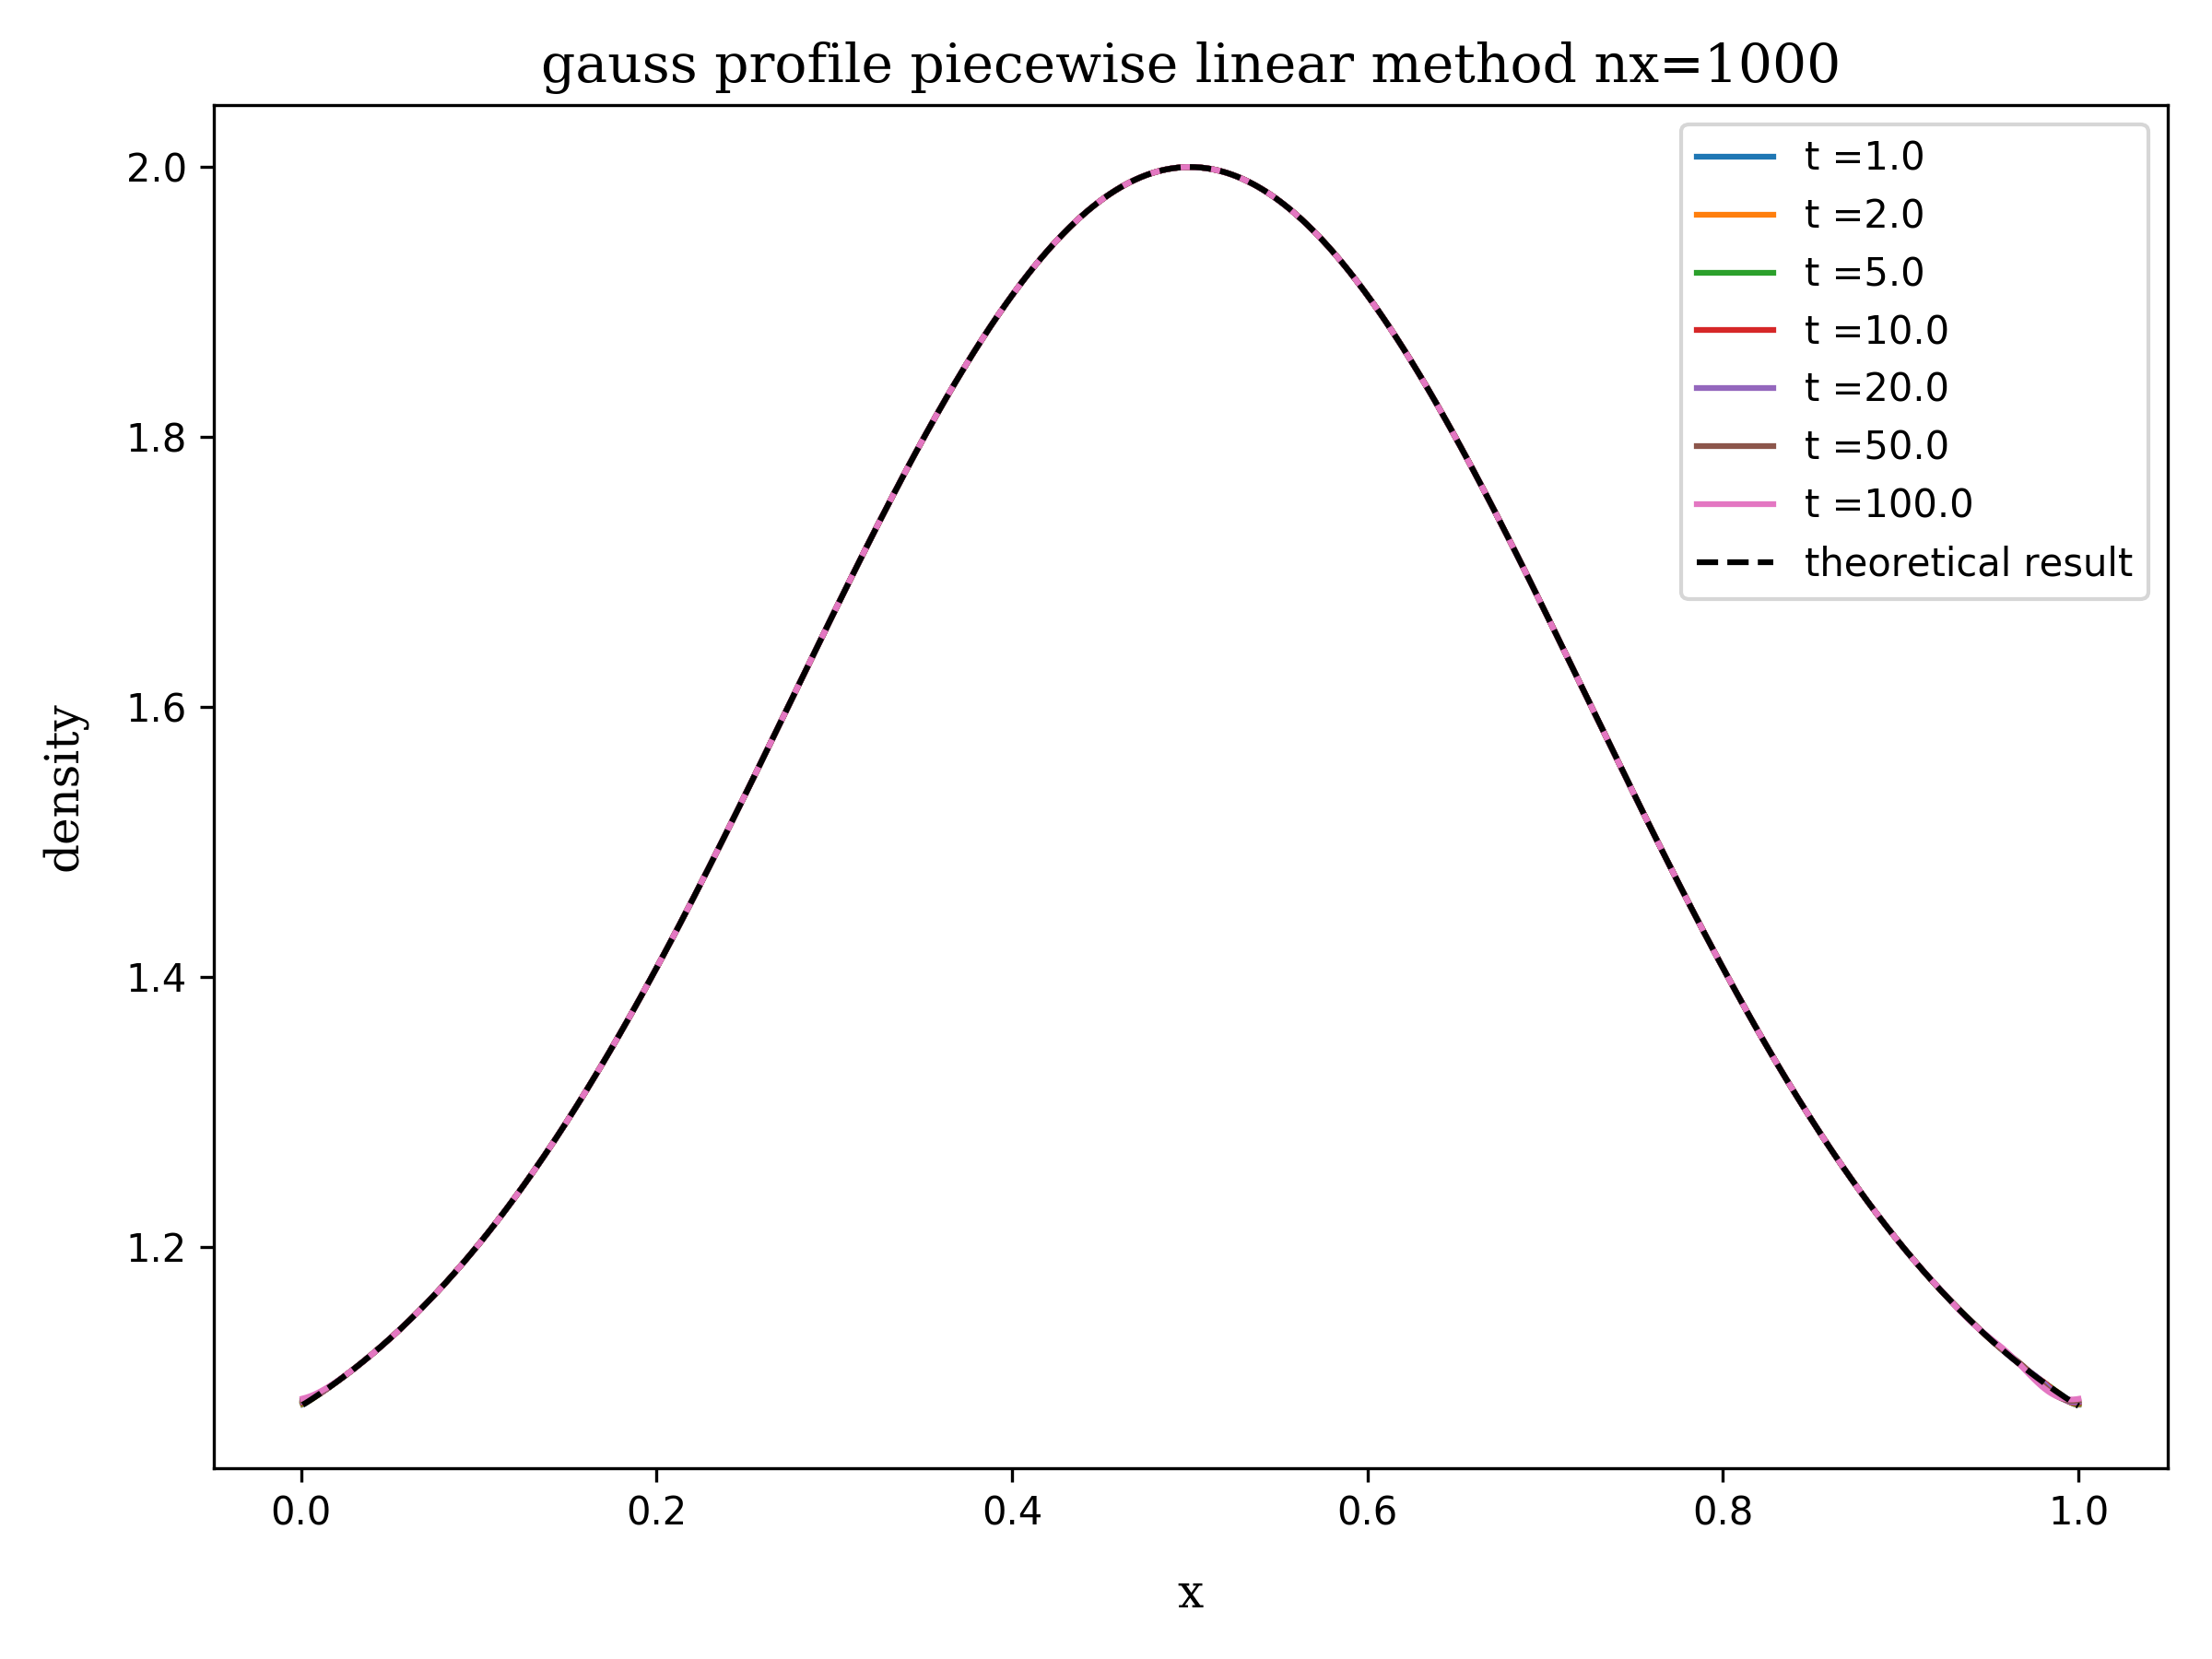
\includegraphics[height=.33\textheight]{../results/1D/pwlin/nx=1000/plot_advection_gauss_pwlin_nx=1000.png}\\
			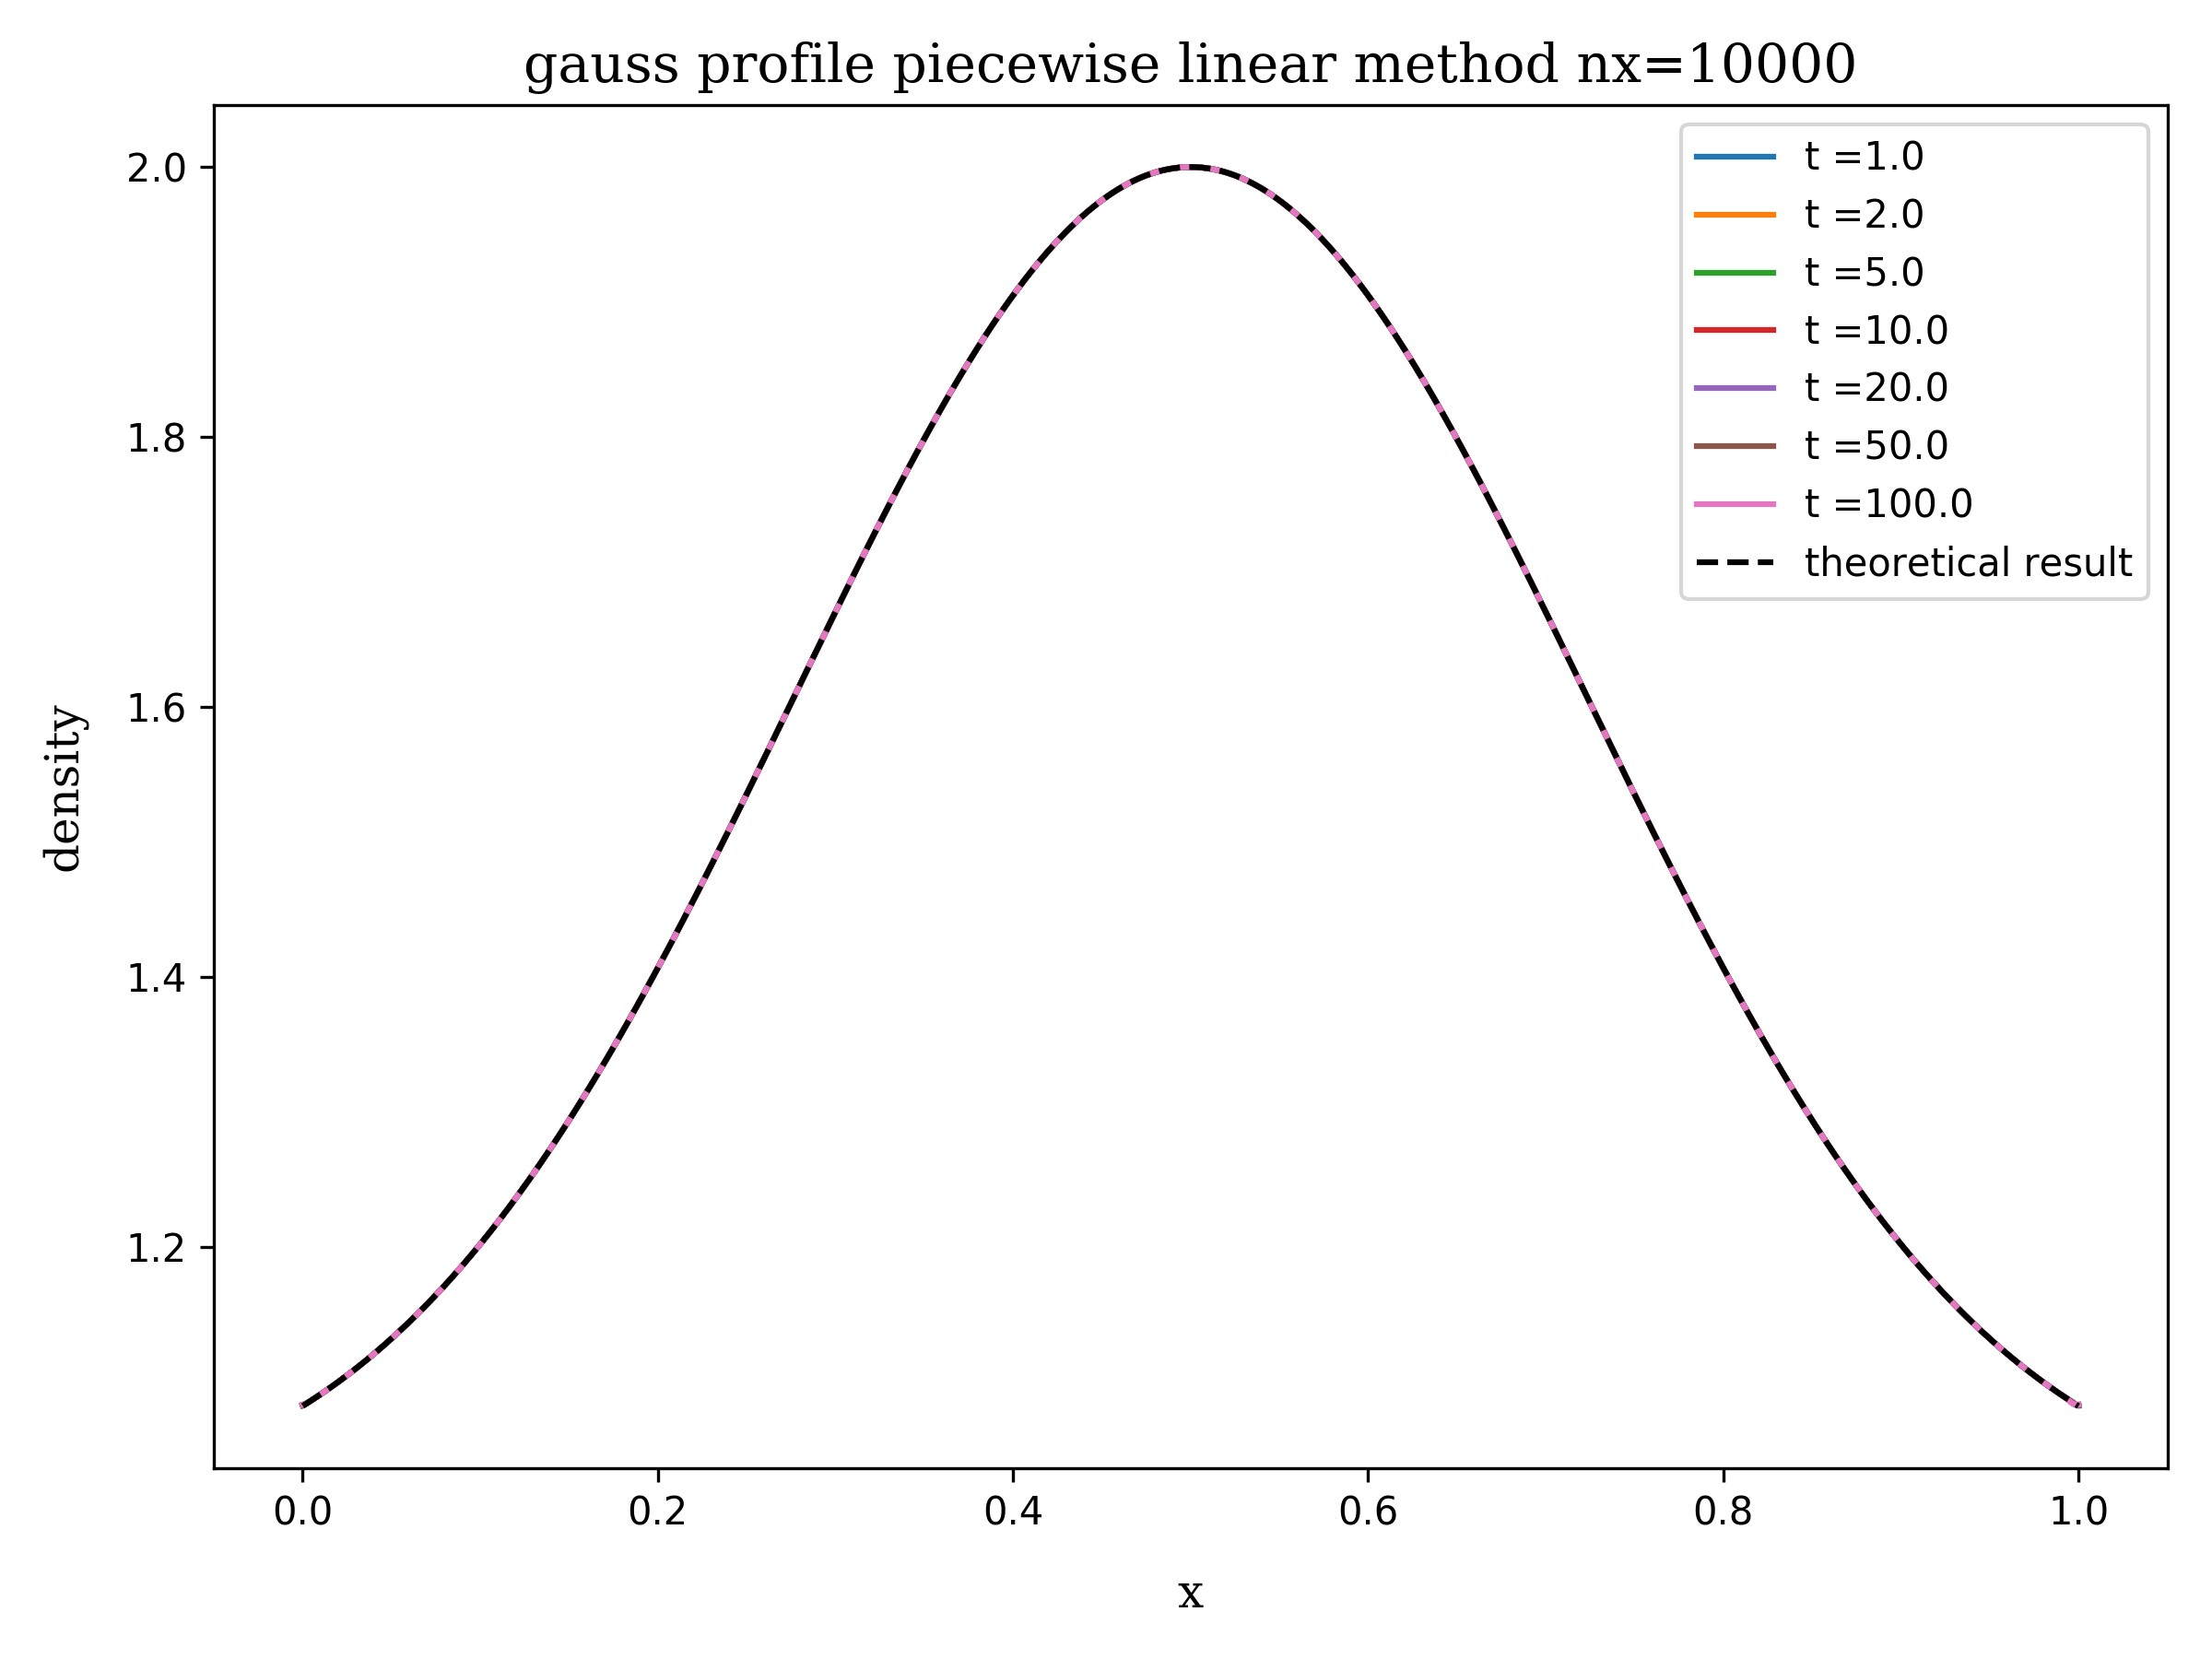
\includegraphics[height=.33\textheight]{../results/1D/pwlin/nx=10000/plot_advection_gauss_pwlin_nx=10000.png}
	\end{columns}
\end{frame}





\begin{frame}
	\begin{block}{New Problem: Oscillations}
		The piecewise linear elements can have overshoots, leading to the oscillations seen in the previous plots.

		
		\begin{center} 
			\includegraphics[height=0.2\textheight]{images/overshoot.png}
			
			\tiny{
				Image adapted from ``Lecture Numerical Fluid Dynamics'', Lecture given by C.P. Dullemond and H.H. Wang at Heidelberg University, 2009
			}
		\end{center}
			
		Godunov's theorem: \textit{any linear algorithm for
			solving partial differential equations, with the property of not producing new extrema, can be at
			most first order.}
		
		$\Rightarrow$ use non-linear conditions (slope limiters) to modify the slope $s_i^n$ to prevent overshoots. Requirement: total variation diminishing: $TV(\rho^{n+1}) \leq TV(\rho^n) \equiv \sum |\rho_i - \rho_{i-1}|$. Such a scheme will not develop oscillations near a jump, because a jump is a monotonically in/decreasing function and a TVD scheme will not increase the $TV$.
	\end{block}
\end{frame}



\section{Minmod Slope Limiter}

\begin{frame}
	\frametitle{Minmod Slope Limiter}
	
	\begin{align*}
		s_i^n = \mathrm{minmod} \left( \frac{\rho_i^n - \rho_{i-1}^n}{\Delta x}, \frac{\rho_{i+1}^n - \rho_i^n}{\Delta x} \right)
	\end{align*}
	with
	\begin{align*}
		\mathrm{minmod}(a, b) = \begin{cases}
		 	a & \text{ if } |a| < |b| \text{ and } ab > 0\\		
		 	b & \text{ if } |a| > |b| \text{ and } ab > 0\\
			0 & \text{ if } ab < 0
								\end{cases}
	\end{align*}
\end{frame}






\begin{frame}
	\vspace{10pt}
	\begin{columns}
		\column{.33\textwidth}
			\centering
			\includegraphics[height=.33\textheight]{../results/1D/minmod/nx=100/plot_advection_step_function_minmod_nx=100.png}\\
			\includegraphics[height=.33\textheight]{../results/1D/minmod/nx=1000/plot_advection_step_function_minmod_nx=1000.png}\\
			\includegraphics[height=.33\textheight]{../results/1D/minmod/nx=10000/plot_advection_step_function_minmod_nx=10000.png}
		\column{.33\textwidth}
			\centering
			\includegraphics[height=.33\textheight]{../results/1D/minmod/nx=100/plot_advection_linear_step_minmod_nx=100.png}\\
			\includegraphics[height=.33\textheight]{../results/1D/minmod/nx=1000/plot_advection_linear_step_minmod_nx=1000.png}\\
			\includegraphics[height=.33\textheight]{../results/1D/minmod/nx=10000/plot_advection_linear_step_minmod_nx=10000.png}
		\column{.33\textwidth}
			\centering
			\includegraphics[height=.33\textheight]{../results/1D/minmod/nx=100/plot_advection_gauss_minmod_nx=100.png}\\
			\includegraphics[height=.33\textheight]{../results/1D/minmod/nx=1000/plot_advection_gauss_minmod_nx=1000.png}\\
			\includegraphics[height=.33\textheight]{../results/1D/minmod/nx=10000/plot_advection_gauss_minmod_nx=10000.png}
	\end{columns}
\end{frame}



\section{Van Leer Slope Limiter}

\begin{frame}
	\frametitle{Van Leer Slope Limiter}
	Rewrite flux (assuming $u = 1$) as
	\begin{align*}
		f_{i-\half}^{n+\half} &= u \rho_{i-1} + \frac{1}{2} u \left( 1 - \frac{u\Delta t}{\Delta x} \right) \phi(r_{i-\half}^n) (q_i^n - q_{i-1}^n)\\
		r_{i-\half}^n &= \frac{q_{i-1}^n - q_{i-2}^n}{q_i^n - q_{i-1}^n}
	\end{align*}
	Here, $\phi$ is the slope/flux limiter.
	
	The Van Leer flux limiter is defined as
	\begin{align*}
		\phi(r) = \frac{r - |r|}{1 - |r|}
	\end{align*}
\end{frame}







%\begin{frame}
%	\vspace{10pt}
%	\begin{columns}
%		\column{.33\textwidth}
%			\centering
%			\includegraphics[height=.33\textheight]{../results/1D/VanLeer/nx=100/plot_advection_step_function_VanLeer_nx=100.png}\\
%			\includegraphics[height=.33\textheight]{../results/1D/VanLeer/nx=1000/plot_advection_step_function_VanLeer_nx=1000.png}\\
%			\includegraphics[height=.33\textheight]{../results/1D/VanLeer/nx=10000/plot_advection_step_function_VanLeer_nx=10000.png}
%		\column{.33\textwidth}
%			\centering
%			\includegraphics[height=.33\textheight]{../results/1D/VanLeer/nx=100/plot_advection_linear_step_VanLeer_nx=100.png}\\
%			\includegraphics[height=.33\textheight]{../results/1D/VanLeer/nx=1000/plot_advection_linear_step_VanLeer_nx=1000.png}\\
%			\includegraphics[height=.33\textheight]{../results/1D/VanLeer/nx=10000/plot_advection_linear_step_VanLeer_nx=10000.png}
%		\column{.33\textwidth}
%			\centering
%			\includegraphics[height=.33\textheight]{../results/1D/VanLeer/nx=100/plot_advection_gauss_VanLeer_nx=100.png}\\
%			\includegraphics[height=.33\textheight]{../results/1D/VanLeer/nx=1000/plot_advection_gauss_VanLeer_nx=1000.png}\\
%			\includegraphics[height=.33\textheight]{../results/1D/VanLeer/nx=10000/plot_advection_gauss_VanLeer_nx=10000.png}
%	\end{columns}
%\end{frame}






\section{Precision of the Algorithms}
\begin{frame}
	\frametitle{Precision of the Algorithms}
	Quantify error through $L1$ error norm: $L1 = \frac{1}{N} \sum\limits_i |\rho_i - \tilde{\rho}(x_i)|$, where $\tilde{\rho}(x_i)$ is the analytical solution.\\[2em]
	
	For $t = 100$:\\\vfill
	
	\begin{columns}
		\column{.37\textwidth}
			\includegraphics[width=\textwidth]{../results/1D/errors/errorplot_advection_step_function_t=100.0.png}
		\column{.37\textwidth}
			\includegraphics[width=\textwidth]{../results/1D/errors/errorplot_advection_linear_step_t=100.0.png}
		\column{.37\textwidth}	
			\includegraphics[width=\textwidth]{../results/1D/errors/errorplot_advection_gauss_t=100.0.png}	
	\end{columns}
	
\end{frame}






\section{2D Advection}

\begin{frame}
	\frametitle{2D Advection}
	
	The 2D advection equation is given by
	\begin{align*}
		\frac{\partial \rho}{\partial t} + u \frac{\partial \rho}{\partial x} + v \frac{\partial \rho}{\partial y} = 0
	\end{align*}
	
	Solution using the same algorithms for each dimension, adding fluxes simultaneously.
	
	Results are shown for a step function density field with $nx = ny = 200$.
	
\end{frame}
\begin{frame}
	\frametitle{$u = 0$, $v = 1$ Piecewise Constant Method}
	%	\vspace{10pt}
	\begin{columns}
		\column{.33\textwidth}
		\centering
		\includegraphics[height=0.4\textheight]{../results/2D/u=0/pwconst/nx=200/plot_advection_2d_step_function_pwconst_nx=200_ny=200t=0.0.png}\\
		\includegraphics[height=0.4\textheight]{../results/2D/u=0/pwconst/nx=200/plot_advection_2d_step_function_pwconst_nx=200_ny=200t=5.0.png}
		\column{.33\textwidth}
		\centering
		\includegraphics[height=0.4\textheight]{../results/2D/u=0/pwconst/nx=200/plot_advection_2d_step_function_pwconst_nx=200_ny=200t=1.0.png}\\
		\includegraphics[height=0.4\textheight]{../results/2D/u=0/pwconst/nx=200/plot_advection_2d_step_function_pwconst_nx=200_ny=200t=10.0.png}
		\column{.33\textwidth}
		\centering
		\includegraphics[height=0.4\textheight]{../results/2D/u=0/pwconst/nx=200/plot_advection_2d_step_function_pwconst_nx=200_ny=200t=2.0.png}\\
		\includegraphics[height=0.4\textheight]{../results/2D/u=0/pwconst/nx=200/plot_advection_2d_step_function_pwconst_nx=200_ny=200t=20.0.png}
	\end{columns}
\end{frame}


\begin{frame}
	\frametitle{$u = 0$, $v = 1$ Piecewise Linear Method}
%	\vspace{10pt}
	\begin{columns}
		\column{.33\textwidth}
			\centering
			\includegraphics[height=0.4\textheight]{../results/2D/u=0/pwlin/nx=200/plot_advection_2d_step_function_pwlin_nx=200_ny=200t=0.0.png}\\
			\includegraphics[height=0.4\textheight]{../results/2D/u=0/pwlin/nx=200/plot_advection_2d_step_function_pwlin_nx=200_ny=200t=5.0.png}
		\column{.33\textwidth}
			\centering
			\includegraphics[height=0.4\textheight]{../results/2D/u=0/pwlin/nx=200/plot_advection_2d_step_function_pwlin_nx=200_ny=200t=1.0.png}\\
			\includegraphics[height=0.4\textheight]{../results/2D/u=0/pwlin/nx=200/plot_advection_2d_step_function_pwlin_nx=200_ny=200t=10.0.png}
		\column{.33\textwidth}
			\centering
			\includegraphics[height=0.4\textheight]{../results/2D/u=0/pwlin/nx=200/plot_advection_2d_step_function_pwlin_nx=200_ny=200t=2.0.png}\\
			\includegraphics[height=0.4\textheight]{../results/2D/u=0/pwlin/nx=200/plot_advection_2d_step_function_pwlin_nx=200_ny=200t=20.0.png}
	\end{columns}
\end{frame}


\begin{frame}
	\frametitle{$u = 0$, $v = 1$ Minmod Slope Limiter}
	%	\vspace{10pt}
	\begin{columns}
		\column{.33\textwidth}
		\centering
		\includegraphics[height=0.4\textheight]{../results/2D/u=0/minmod/nx=200/plot_advection_2d_step_function_minmod_nx=200_ny=200t=0.0.png}\\
		\includegraphics[height=0.4\textheight]{../results/2D/u=0/minmod/nx=200/plot_advection_2d_step_function_minmod_nx=200_ny=200t=5.0.png}
		\column{.33\textwidth}
		\centering
		\includegraphics[height=0.4\textheight]{../results/2D/u=0/minmod/nx=200/plot_advection_2d_step_function_minmod_nx=200_ny=200t=1.0.png}\\
		\includegraphics[height=0.4\textheight]{../results/2D/u=0/minmod/nx=200/plot_advection_2d_step_function_minmod_nx=200_ny=200t=10.0.png}
		\column{.33\textwidth}
		\centering
		\includegraphics[height=0.4\textheight]{../results/2D/u=0/minmod/nx=200/plot_advection_2d_step_function_minmod_nx=200_ny=200t=2.0.png}\\
		\includegraphics[height=0.4\textheight]{../results/2D/u=0/minmod/nx=200/plot_advection_2d_step_function_minmod_nx=200_ny=200t=20.0.png}
	\end{columns}
\end{frame}




\begin{frame}
	\frametitle{$u = 0$, $v = 1$ Van Leer Slope Limiter}
	%	\vspace{10pt}
	\begin{columns}
		\column{.33\textwidth}
		\centering
		\includegraphics[height=0.4\textheight]{../results/2D/u=0/VanLeer/nx=200/plot_advection_2d_step_function_VanLeer_nx=200_ny=200t=0.0.png}\\
		\includegraphics[height=0.4\textheight]{../results/2D/u=0/VanLeer/nx=200/plot_advection_2d_step_function_VanLeer_nx=200_ny=200t=5.0.png}
		\column{.33\textwidth}
		\centering
		\includegraphics[height=0.4\textheight]{../results/2D/u=0/VanLeer/nx=200/plot_advection_2d_step_function_VanLeer_nx=200_ny=200t=1.0.png}\\
		\includegraphics[height=0.4\textheight]{../results/2D/u=0/VanLeer/nx=200/plot_advection_2d_step_function_VanLeer_nx=200_ny=200t=10.0.png}
		\column{.33\textwidth}
		\centering
		\includegraphics[height=0.4\textheight]{../results/2D/u=0/VanLeer/nx=200/plot_advection_2d_step_function_VanLeer_nx=200_ny=200t=2.0.png}\\
		\includegraphics[height=0.4\textheight]{../results/2D/u=0/VanLeer/nx=200/plot_advection_2d_step_function_VanLeer_nx=200_ny=200t=20.0.png}
	\end{columns}
\end{frame}



\begin{frame}
	\frametitle{$u = 1$, $v = 0$ Piecewise Constant Method}
	%	\vspace{10pt}
	\begin{columns}
		\column{.33\textwidth}
		\centering
		\includegraphics[height=0.4\textheight]{../results/2D/u=1/pwconst/nx=200/plot_advection_2d_step_function_pwconst_nx=200_ny=200t=0.0.png}\\
		\includegraphics[height=0.4\textheight]{../results/2D/u=1/pwconst/nx=200/plot_advection_2d_step_function_pwconst_nx=200_ny=200t=5.0.png}
		\column{.33\textwidth}
		\centering
		\includegraphics[height=0.4\textheight]{../results/2D/u=1/pwconst/nx=200/plot_advection_2d_step_function_pwconst_nx=200_ny=200t=1.0.png}\\
		\includegraphics[height=0.4\textheight]{../results/2D/u=1/pwconst/nx=200/plot_advection_2d_step_function_pwconst_nx=200_ny=200t=10.0.png}
		\column{.33\textwidth}
		\centering
		\includegraphics[height=0.4\textheight]{../results/2D/u=1/pwconst/nx=200/plot_advection_2d_step_function_pwconst_nx=200_ny=200t=2.0.png}\\
		\includegraphics[height=0.4\textheight]{../results/2D/u=1/pwconst/nx=200/plot_advection_2d_step_function_pwconst_nx=200_ny=200t=20.0.png}
	\end{columns}
\end{frame}


\begin{frame}
	\frametitle{$u = 1$, $v = 0$ Piecewise Linear Method}
%	\vspace{10pt}
	\begin{columns}
		\column{.33\textwidth}
			\centering
			\includegraphics[height=0.4\textheight]{../results/2D/u=1/pwlin/nx=200/plot_advection_2d_step_function_pwlin_nx=200_ny=200t=0.0.png}\\
			\includegraphics[height=0.4\textheight]{../results/2D/u=1/pwlin/nx=200/plot_advection_2d_step_function_pwlin_nx=200_ny=200t=5.0.png}
		\column{.33\textwidth}
			\centering
			\includegraphics[height=0.4\textheight]{../results/2D/u=1/pwlin/nx=200/plot_advection_2d_step_function_pwlin_nx=200_ny=200t=1.0.png}\\
			\includegraphics[height=0.4\textheight]{../results/2D/u=1/pwlin/nx=200/plot_advection_2d_step_function_pwlin_nx=200_ny=200t=10.0.png}
		\column{.33\textwidth}
			\centering
			\includegraphics[height=0.4\textheight]{../results/2D/u=1/pwlin/nx=200/plot_advection_2d_step_function_pwlin_nx=200_ny=200t=2.0.png}\\
			\includegraphics[height=0.4\textheight]{../results/2D/u=1/pwlin/nx=200/plot_advection_2d_step_function_pwlin_nx=200_ny=200t=20.0.png}
	\end{columns}
\end{frame}


\begin{frame}
	\frametitle{$u = 1$, $v = 0$ Minmod Slope Limiter}
	%	\vspace{10pt}
	\begin{columns}
		\column{.33\textwidth}
		\centering
		\includegraphics[height=0.4\textheight]{../results/2D/u=1/minmod/nx=200/plot_advection_2d_step_function_minmod_nx=200_ny=200t=0.0.png}\\
		\includegraphics[height=0.4\textheight]{../results/2D/u=1/minmod/nx=200/plot_advection_2d_step_function_minmod_nx=200_ny=200t=5.0.png}
		\column{.33\textwidth}
		\centering
		\includegraphics[height=0.4\textheight]{../results/2D/u=1/minmod/nx=200/plot_advection_2d_step_function_minmod_nx=200_ny=200t=1.0.png}\\
		\includegraphics[height=0.4\textheight]{../results/2D/u=1/minmod/nx=200/plot_advection_2d_step_function_minmod_nx=200_ny=200t=10.0.png}
		\column{.33\textwidth}
		\centering
		\includegraphics[height=0.4\textheight]{../results/2D/u=1/minmod/nx=200/plot_advection_2d_step_function_minmod_nx=200_ny=200t=2.0.png}\\
		\includegraphics[height=0.4\textheight]{../results/2D/u=1/minmod/nx=200/plot_advection_2d_step_function_minmod_nx=200_ny=200t=20.0.png}
	\end{columns}
\end{frame}




\begin{frame}
	\frametitle{$u = 1$, $v = 0$ Van Leer Slope Limiter}
	%	\vspace{10pt}
	\begin{columns}
		\column{.33\textwidth}
		\centering
		\includegraphics[height=0.4\textheight]{../results/2D/u=1/VanLeer/nx=200/plot_advection_2d_step_function_VanLeer_nx=200_ny=200t=0.0.png}\\
		\includegraphics[height=0.4\textheight]{../results/2D/u=1/VanLeer/nx=200/plot_advection_2d_step_function_VanLeer_nx=200_ny=200t=5.0.png}
		\column{.33\textwidth}
		\centering
		\includegraphics[height=0.4\textheight]{../results/2D/u=1/VanLeer/nx=200/plot_advection_2d_step_function_VanLeer_nx=200_ny=200t=1.0.png}\\
		\includegraphics[height=0.4\textheight]{../results/2D/u=1/VanLeer/nx=200/plot_advection_2d_step_function_VanLeer_nx=200_ny=200t=10.0.png}
		\column{.33\textwidth}
		\centering
		\includegraphics[height=0.4\textheight]{../results/2D/u=1/VanLeer/nx=200/plot_advection_2d_step_function_VanLeer_nx=200_ny=200t=2.0.png}\\
		\includegraphics[height=0.4\textheight]{../results/2D/u=1/VanLeer/nx=200/plot_advection_2d_step_function_VanLeer_nx=200_ny=200t=20.0.png}
	\end{columns}
\end{frame}



\begin{frame}
	\frametitle{$u = v = \sqrt{2}/2$ Piecewise Constant Method}
	%	\vspace{10pt}
	\begin{columns}
		\column{.33\textwidth}
		\centering
		\includegraphics[height=0.4\textheight]{../results/2D/u=0.5sqrt(2)/pwconst/nx=200/plot_advection_2d_step_function_pwconst_nx=200_ny=200t=0.0.png}\\
		\includegraphics[height=0.4\textheight]{../results/2D/u=0.5sqrt(2)/pwconst/nx=200/plot_advection_2d_step_function_pwconst_nx=200_ny=200t=5.0.png}
		\column{.33\textwidth}
		\centering
		\includegraphics[height=0.4\textheight]{../results/2D/u=0.5sqrt(2)/pwconst/nx=200/plot_advection_2d_step_function_pwconst_nx=200_ny=200t=1.0.png}\\
		\includegraphics[height=0.4\textheight]{../results/2D/u=0.5sqrt(2)/pwconst/nx=200/plot_advection_2d_step_function_pwconst_nx=200_ny=200t=10.0.png}
		\column{.33\textwidth}
		\centering
		\includegraphics[height=0.4\textheight]{../results/2D/u=0.5sqrt(2)/pwconst/nx=200/plot_advection_2d_step_function_pwconst_nx=200_ny=200t=2.0.png}\\
		\includegraphics[height=0.4\textheight]{../results/2D/u=0.5sqrt(2)/pwconst/nx=200/plot_advection_2d_step_function_pwconst_nx=200_ny=200t=20.0.png}
	\end{columns}
\end{frame}


\begin{frame}
	\frametitle{$u = v = \sqrt{2}/2$ Piecewise Linear Method}
%	\vspace{10pt}
	\begin{columns}
		\column{.33\textwidth}
			\centering
			\includegraphics[height=0.4\textheight]{../results/2D/u=0.5sqrt(2)/pwlin/nx=200/plot_advection_2d_step_function_pwlin_nx=200_ny=200t=0.0.png}\\
			\includegraphics[height=0.4\textheight]{../results/2D/u=0.5sqrt(2)/pwlin/nx=200/plot_advection_2d_step_function_pwlin_nx=200_ny=200t=5.0.png}
		\column{.33\textwidth}
			\centering
			\includegraphics[height=0.4\textheight]{../results/2D/u=0.5sqrt(2)/pwlin/nx=200/plot_advection_2d_step_function_pwlin_nx=200_ny=200t=1.0.png}\\
			\includegraphics[height=0.4\textheight]{../results/2D/u=0.5sqrt(2)/pwlin/nx=200/plot_advection_2d_step_function_pwlin_nx=200_ny=200t=10.0.png}
		\column{.33\textwidth}
			\centering
			\includegraphics[height=0.4\textheight]{../results/2D/u=0.5sqrt(2)/pwlin/nx=200/plot_advection_2d_step_function_pwlin_nx=200_ny=200t=2.0.png}\\
			\includegraphics[height=0.4\textheight]{../results/2D/u=0.5sqrt(2)/pwlin/nx=200/plot_advection_2d_step_function_pwlin_nx=200_ny=200t=20.0.png}
	\end{columns}
\end{frame}


\begin{frame}
	\frametitle{$u = v = \sqrt{2}/2$ Minmod Slope Limiter}
	%	\vspace{10pt}
	\begin{columns}
		\column{.33\textwidth}
		\centering
		\includegraphics[height=0.4\textheight]{../results/2D/u=0.5sqrt(2)/minmod/nx=200/plot_advection_2d_step_function_minmod_nx=200_ny=200t=0.0.png}\\
		\includegraphics[height=0.4\textheight]{../results/2D/u=0.5sqrt(2)/minmod/nx=200/plot_advection_2d_step_function_minmod_nx=200_ny=200t=5.0.png}
		\column{.33\textwidth}
		\centering
		\includegraphics[height=0.4\textheight]{../results/2D/u=0.5sqrt(2)/minmod/nx=200/plot_advection_2d_step_function_minmod_nx=200_ny=200t=1.0.png}\\
		\includegraphics[height=0.4\textheight]{../results/2D/u=0.5sqrt(2)/minmod/nx=200/plot_advection_2d_step_function_minmod_nx=200_ny=200t=10.0.png}
		\column{.33\textwidth}
		\centering
		\includegraphics[height=0.4\textheight]{../results/2D/u=0.5sqrt(2)/minmod/nx=200/plot_advection_2d_step_function_minmod_nx=200_ny=200t=2.0.png}\\
		\includegraphics[height=0.4\textheight]{../results/2D/u=0.5sqrt(2)/minmod/nx=200/plot_advection_2d_step_function_minmod_nx=200_ny=200t=20.0.png}
	\end{columns}
\end{frame}




\begin{frame}
	\frametitle{$u = v = \sqrt{2}/2$ Van Leer Slope Limiter}
	%	\vspace{10pt}
	\begin{columns}
		\column{.33\textwidth}
		\centering
		\includegraphics[height=0.4\textheight]{../results/2D/u=0.5sqrt(2)/VanLeer/nx=200/plot_advection_2d_step_function_VanLeer_nx=200_ny=200t=0.0.png}\\
		\includegraphics[height=0.4\textheight]{../results/2D/u=0.5sqrt(2)/VanLeer/nx=200/plot_advection_2d_step_function_VanLeer_nx=200_ny=200t=5.0.png}
		\column{.33\textwidth}
		\centering
		\includegraphics[height=0.4\textheight]{../results/2D/u=0.5sqrt(2)/VanLeer/nx=200/plot_advection_2d_step_function_VanLeer_nx=200_ny=200t=1.0.png}\\
		\includegraphics[height=0.4\textheight]{../results/2D/u=0.5sqrt(2)/VanLeer/nx=200/plot_advection_2d_step_function_VanLeer_nx=200_ny=200t=10.0.png}
		\column{.33\textwidth}
		\centering
		\includegraphics[height=0.4\textheight]{../results/2D/u=0.5sqrt(2)/VanLeer/nx=200/plot_advection_2d_step_function_VanLeer_nx=200_ny=200t=2.0.png}\\
		\includegraphics[height=0.4\textheight]{../results/2D/u=0.5sqrt(2)/VanLeer/nx=200/plot_advection_2d_step_function_VanLeer_nx=200_ny=200t=20.0.png}
	\end{columns}
\end{frame}









\begin{frame}[fragile]
	Program, plotting scripts and this presentation available on \verb!https://bitbucket.org/mivkov/computational_astrophysics!
\end{frame}













\end{document}
